\documentclass[a4paper, 12pt]{book}
\usepackage[top=3cm,bottom=2cm,left=2cm,right=2cm,headsep=10pt]{geometry}
%\geometry{
%    papersize={155.57mm, 234.95mm},
%    layoutsize={152.4mm, 228.61mm},
%    layoutoffset = {1.58mm,1.58mm},
%    bindingoffset = -1.27mm,
%    showcrop,
%}

\usepackage{fancyhdr}
\usepackage{graphicx}
\usepackage{xcolor} % Required for specifying colors by name
\definecolor{bg}{rgb}{0.95,0.95,0.95}
\definecolor{ocre}{RGB}{52,177,201} % Define the orange color used for highlighting throughout the book
\definecolor{exer}{HTML}{A5C5F5}
\definecolor{exertitle}{RGB}{52,177,201}
\definecolor{notecolor}{RGB}{100, 149, 237}
\definecolor{warncolor}{RGB}{255, 59, 0}
\definecolor{warntitle}{RGB}{255, 59, 0}
\usepackage{hyperref}
\usepackage{fontspec}

\setmainfont[Path = /usr/share/texlive/texmf-dist/fonts/opentype/public/libertinus/,
BoldFont = libertinussans-bold,
ItalicFont = libertinussans-italic,
]{libertinussans-regular}

\setmonofont[Scale=MatchLowercase, Path = /usr/share/texlive/texmf-dist/fonts/opentype/adobe/sourcecodepro/]{SourceCodePro-Regular.otf}

\usepackage{pdfpages}
\usepackage{polyglossia}
\setmainlanguage{english}
\hyphenpenalty=1000 % default 50
\tolerance=500      % default 200

\usepackage[titletoc]{appendix}
\usepackage{titlesec} % Allows customization of titles
\usepackage{tcolorbox}

\usepackage[utf8]{inputenc}

\usepackage{minted}
\setminted{breaklines, autogobble, fontsize=\footnotesize}
\setminted[]{bgcolor=bg}

\newenvironment{warning}[1]{%
    \begin{tcolorbox}[width=\textwidth,colframe={warncolor}, colback=red!5!white, title={Warning}, outer arc=2mm]
    {#1}
    \end{tcolorbox}
}

\newenvironment{note}[1]{%
    \begin{tcolorbox}[width=\textwidth,colframe={notecolor}, colback=blue!5!white, title={Note}, outer arc=2mm]
    {#1}
    \end{tcolorbox}
}

\newenvironment{exercise}[1]{%
    \begin{tcolorbox}[width=\textwidth,colframe={exertitle}, colback={exer}, title={Exercise},outer arc=2mm]
    {#1}
    \end{tcolorbox}
}

\newenvironment{py}[1]{\mintinline{python}{#1}}

\title{Python For The Lab}
\author{Aquiles Carattino}

\begin{document}
    \frontmatter

    \includepdf[pages=-]{cover-pftl.pdf}

    \clearpage
%% temporary titles
% command to provide stretchy vertical space in proportion
\newcommand\nbvspace[1][3]{\vspace*{\stretch{#1}}}
% allow some slack to avoid under/overfull boxes
\newcommand\nbstretchyspace{\spaceskip0.5em plus 0.25em minus 0.25em}
% To improve spacing on titlepages
\newcommand{\nbtitlestretch}{\spaceskip0.6em}
\pagestyle{empty}
\begin{center}
\bfseries
\nbvspace[1]
\Huge
{\nbtitlestretch\huge
PYTHON FOR THE LAB}

\nbvspace[1]
\normalsize

AN INTRODUCTION TO SOLVING\\
THE MOST COMMON PROBLEMS\\
A SCIENTIST FACES IN THE LAB \\

\nbvspace[1]
\small BY\\
\Large AQUILES CARATTINO\\[0.5em]
\footnotesize PhD IN PHYSICS, SOFTWARE DEVELOPER 

\nbvspace[2]


\includegraphics[width=1.5in]{./images/Floral-Silhouette-2.png}
\nbvspace[3]
\normalsize

AMSTERDAM\\
\large
2018
\nbvspace[1]
\end{center}


    \newpage
    \tableofcontents
    \mainmatter
    \chapter{Introduction}
In most laboratories around the world, computers are in charge of controlling experiments. From complex systems such as particle accelerators to simpler UV-Vis spectrometers, there is always a computer in charge of asking the user for some input, performing a measurement and displaying the results. However, for many experimentalists, the software that comes packaged is not sufficient and is barely customizable. Moreover, if you have a custom built setup you will also need custom built software.

Even if most scientists are used to analyzing data with a computer, very few of them are able to write software for controlling experiments. This is due, in part, to a very severe lack of documentation and examples, in part due to the lack of working libraries to work upon. Python For The Lab is a humble attempt to overcome the current limitations while trying to build a community around common practices when dealing with experiments and interfacing through the computer.

Without further ado, welcome to the book Python For The Lab. This book is thought as a guide to building all the software you need for interfacing with a real-world device. We are going to start from the very basic of communicating with a device through the exchange of commands, building slowly towards classes and finalizing with a graphical user interfaces (GUI). This book is task-oriented, meaning that it is focused on showing you how things can be done and not into a lot of theory on how programming works in general. This, of course, leads to some generalizations that may not be correct in all scenarios. I ask your forgiveness in those cases and your cooperation: if you find anything that can be improved, or corrected, please contact me.

Together with the book, there is a website where you can find extra information, anecdotes and examples that didn’t fit in here. Remember that the website is the proper place to communicate with fellow Python For The Lab readers. If you are stuck with the exercises or you have questions that are not answered in the book, don’t hesitate to shout in the comments section of the website.

This book is a compendium of the best strategies that I have found while developing software for different laboratories. I have tried to justify every decision made, but some are more of an aesthetic choice than an architectural one. You are free to change and improve whatever you think will lead you to better (or faster) results. I have tested what I propose and I am very confident with the outcome. If you are not very experienced, I suggest that you start in the same way as the book does and later on you can find your own way.

When developing software, you will probably realize that it is going to be used by another person either at the same time or in the future. In many labs, people come and go and therefore you cannot count on being around for answering questions regarding your programs, or vice versa, you will have to understand someone else’s code. If you adhere to some common standards, everybody’s life will be much easier, and in Python For The Lab, you will find a lot of recommendations regarding how to make your code clear, to you and to others.

You can find many tools that will help you in keeping your code organized, such as tools for version control and documenting. They are, however, a topic completely different from what we intend to cover in this book. There will be some hints as to where to start. Remember that many of the problems can be solved by clear policies established in each lab, such as where to put the code for sharing with other members, how to document, etc. If there is nothing like that where you work, you should seriously consider discussing it with your team members.

The book is divided into different chapters where you will develop different skills. Each chapter is aimed at tackling a specific problem that we want to solve, and that is clearly stated in the chapter objectives. It may happen that a chapter is easier for you because it is what you are used to doing, and you will be inclined to skip it. However, bear in mind that each chapter builds on the previous one and therefore you should be sure that you have the needed code in place.

\section{Who is this book intended for}
When I started this book I wanted to make it possible for people with very different programming levels to achieve a common goal. I found that the only way to do this is to be a bit dogmatic with the explanations, for example, if you want to do this you should type that. By starting the development through a real need, a question arising from the real world, you can anticipate what is going to happen in the future and therefore the motivation level will remain high enough as to continue thinking in a solution.

Generally speaking, you will need a bit of programming knowledge; you should understand what an if statement is, why would you use a for loop or a while loop. We are going to make extensive use of classes in Python, but without complicating it too much. In the book, you can find a refreshment of how to work with classes and other syntactic examples of Python. You should read that chapter through, especially if you are not familiar with Python. If you find that the contents are too complicated for your level, you should consider starting with an easier book, perhaps on how to use Python for analyzing data.

Even if not strictly required, you will also need a basic understanding of how an experiment works and a bit of physics. Namely, you need to understand that an experiment starts by designing a way in which you can alter your object of study in a controlled manner and monitor some signals while you do so. The experiment we are going to perform throughout this book is a common example in many, many different fields: we are going to change an analog output while we measure an analog input. If you are using the device that accompanies the course, the experiment is going to be measuring the I-V curve of a diode.

\section{What do we want to achieve?}

With this book we want you to gain a first insight into the world of developing software for controlling experiments. Not only through the command line but also through a User Interface that you are going to build yourself from scratch. We want to lay down the foundations for future work in developing an ecosystem of packages that can control a variety of experiments, in different fields.

By following the book you will gain a set of tools that you will be able to immediately use in your own laboratory. It may seem simple at the beginning, but if you think it through, you will notice that the possibilities are endless. The main objective of this book is to give you the tools to be able to understand the documentation online and to know where you can ask for help.

By reading the book you are not going to become a better programmer; you are not going to learn the fancy caveats of Python such as decorators, inheritance, etc. But you will learn how to package your code for others to use, how to use threading for performing different tasks at the same time and many other useful topics for working in the lab. It is a very hands-on approach that has proven to be the best pedagogical strategy.

You are going to receive a device that will act as a DAQ, short of Data Acquisition. The device is able to acquire analog signals but also to generate analog outputs. They are called analog because you can set the output to whatever value you want within a certain voltage range. The device will be connected to the computer via the USB port. With this device you are going to perform an experiment: measure the I-V curve of a diode. This is, measure the current that circulates through a diode as a function of the voltage that you apply to it.

Varying an output voltage and recording an input is a common task in innumerable experiments from different fields. Changing a voltage can be related to displacement through a piezo stage, you can change the intensity of light, you can alter temperature and the list goes on and on. Measuring a voltage can be equivalent to determining a current, the intensity of light, a displacement, a force, etc. Most likely at your own lab, you will find this same pattern.

What we want to achieve therefore is not just measuring the I-V curve of a diode, but showing you all the process from building a driver for your device, to performing a measurement and building a user interface to interact with it. The skills that you are going to acquire are the base for building very sophisticated and specialized software. You are also going to get acquainted with resources and tools that you will find very interesting for the future.

\section{Why Python?}

Python became ubiquitous in many research labs because of many different reasons. First, Python is free and open source and therefore there is no overhead when implementing it. Compared to the price of the licenses of programs such as Matlab or LabView, we can make some compromises while using Python. On the downside, Matlab and Lab View have a relatively good professional support and communities built around them. Answers to questions regarding Python have to be found by searching online, most likely in Stack Overflow.

If you search online for instructions on how to control your experiment with Python, you will find really few sources of information. Fortunately, this is changing thanks to an evergrowing number of people developing open source code and writing very useful documentation. Python can achieve all the same functionality as Lab View, the only limitation is the existence of drivers for more complex instruments. With a stronger community, companies will realize the value of providing drivers for other programming environments.

Python doesn’t need to be compiled to execute a script, meaning that changes done to the code can be immediately observed. Its syntax is very clear and intuitive; people making the switch from Matlab will find no problems in understanding the code. People making the switch from LabView, however, will have a higher learning curve converting from a drag-and-drop approach to a normal typed language. In any case, once some syntactic elements are known, a lot of things can be programmed.

A very important aspect of Python is that it is platform independent. Since Python is interpreted by a special program every time we run it, it will produce the same output regardless of whether we run on Linux, Windows or Mac. The python interpreter is responsible for adapting the way our code works under the hood to the different architectures. Thus we can develop on our office PC running Windows, run the code in the lab that runs Linux and share it with a colleague who prefers a Mac.

Many of the doubts that can arise when programming with Python will not be specific to interfacing with instruments, but more general regarding how to achieve a certain functionality. Normally you can find answers to all of them just by searching online. And if not, a great source of information is Stack Overflow. Don’t be afraid to ask whatever is in your mind, the community will guide you through the process on how to make your question more specific if needed, or they will point you towards the solution.

\section{The Onion Principle}

When you start developing software it is very hard to think ahead. Most likely you have a small problem that you want to solve and you just go for it. Later on, it may turn out, and this is especially true for people who work in labs, that that small problem is actually something worth investigating. Your software will not be able to handle the new tasks and you will need to improve it. Here is where having the proper set of rules in place will help you and I like to call them the Onion Principle.

The rules I am talking about are not rules written in stone and that you can find clearly stated in a book (by the way, you won’t find them here). I am talking about a set of mind that will empower yourself to develop better, clearer and more expandable code. Sitting down and reflecting is the best you can do, even more than sitting down and typing. When dealing with experiments you have a lot of things to ask yourself, what do you know, what do you want to prove, how to do it. Only then you will sit down to write a program that responds to your needs.

If you build something that cannot be expanded, it will become useless very soon. When you don’t really know what may happen with your code, you should think ahead and structure it as an onion, in layers. I am not claiming that it is something that happens naturally, but you can develop your own set of procedures to ensure that you are developing future-proof code. Once you get the handle of it, it won’t take you longer than being disorganized and not having the proper structure. Variables that are not self-descriptive, lack comments, and the list goes on and on.

It is not all about being future-proof. When you start with a simple task at hand, you want to solve it quickly and not spending hours developing useless lines of code just thinking what if. I am all in for that kind of solutions; however, a strong foundation is always important. Taking shortcuts just because you don’t want to create a separated file will give you more headaches even in the short term. You should build code that is robust enough to support for expansion later on. In the same way that you take steps while performing an experiment, you should take steps when developing software.

One of the key elements to achieve a great onion-like approach in Python is to use classes. They are concise elements with clear functionality and very easy to document. They can be imported and even expanded without changing the original code, as we will see by the end of this chapter. If you come from the data analysis world, it may very well be that you never developed your own classes, but this is about to change with this book. You shouldn’t be afraid of them; you should just try to understand them because I can guarantee that once you get the handle of the, you won’t be able to stop thinking in their own terms.

I will not make special emphasis on why I ask you to do the things in a certain way throughout the book. However, if you pay attention you will notice that each step is incremental. You won’t have to start all over again to add a new feature that you didn’t about. And this ends up being easy because the foundation given by the previous step is very solid. I am not saying that there is only one way of achieving the same results, but I will be just showing you a way of doing things. When you have the chance to improve something without much effort, you should take it, you will be very grateful to your past self.

In the end, all the common practices and development patterns that I can show you, are thought just to make you save time not only in the long run but also next week. I have, just as you are about to do, started developing software for acquiring a very simple signal, an analog input generated by a photodiode. It didn’t take long until I wanted to move a piezo stage with an analog output and suddenly I needed a way of doing 2D and 3D scans of my sample. Sadly for me, there was no one around who could show me a way to being organized and clear with my code.

This book is based not only on my own experiences working in different labs but also on the experiences of the people who surrounded me, who received my code. Sometimes we cannot anticipate the ramifications that our work will have, but I can assure to you, that if you started like a small onion, layer by layer, they are going to be very satisfying.

\section{The Agile Process}

The Agile software development describes a particular approach to software development methodology based on iterative development. Its core value is that requirements and solutions evolve through a collaborative process between developers and customers. The principles of the Agile methodology are summarized in four statements in its manifesto. They are:

        Individuals and interactions over processes and tools
        Working software over comprehensive documentation
        Customer collaboration over contract negotiation
        Responding to change over following a plan

Agile in itself doesn’t establish any particulars regarding programming but just how to develop a workflow and a working environment. In the last few years, Agile has attracted a lot of attention, extending its concepts away from software development, and moving into project management. Even though the core principles were drawn from a programming context, scientific projects could also benefit from the Agile ideas, but with some reservations.

Some of the main points of an Agile process, such as responding to change over following a plan are a routine reality in a lab. Plans are hard to follow because a researcher cannot be sure of what lays ahead. More interesting questions arise or some things just don’t work as expected. Being flexible to overcome obstacles and to change focus when more important questions can be answered, is a needed attribute of successful researchers.

Collaboration over negotiation is also common in a scientific setting, where a lot of agreements are done verbally, without almost any negotiation. Sometimes it is not even an agreement, but just mere curiosity that sparkles a collaboration. Collaboration in science often starts with complementary capacities, for example, two different groups which developed expertise in different techniques. Negotiations come at a much later stage, only when the collaboration was successful and researchers need to agree on how to share the credit.

The other two principles of the Agile methodology, however, are worth discussing in detail in the context of scientific work. To value individuals and interactions is a general principle to which few researchers will oppose. It is better to allow creativity than to be fixated on a specific process or tool. Moreover, great ideas may appear from a discussion or an interaction with another researcher. However, it is also important to value the processes and tools that each researcher has available in the lab. Even though questions can appear in any setting, only places with the proper setups will be able to answer them. The opposite is also valid, posing questions to which one has the proper tools to answer.

The context of every research is different and every field is particular; valuing individuals is part of a healthy working environment, but one should not lose sight of the established processes. Processes can guarantee the quality of data and the moral integrity of researchers. It doesn’t mean things cannot be changed for the better, but there should be a limit to how much an individual can be valued over an established process. A brilliant scientist will stop contributing to the group if he or she doesn’t document the work or doesn’t follow the procedures established to share resources, for example.

Working software over extensive documentation should be better rephrased as Results over extensive documentation. In this particular point, an Agile process can be the opposite of what a lab manager wishes, but it is exactly what commonly happens. Reproducing results is only possible when extensive documentation is available, allowing others to perform the exact same measurement. The pace at which science is moving, however, values quick results over thorough research, allowing little or no time to provide extensive documentation about experiments and results.

Documentation in science has a different value than for software development, but the rhythm at which both evolve is fundamentally the same. Science is based on building on each other’s work, while software development can be done to overcome a very specific obstacle. The difference between a scientific work and software development is, therefore, the life cycle of the results. While one expects to build experiments on top of the knowledge generated in a lab, he may not use an available program as a starting point for further development.

The Agile manifesto provides not only the four values stated at the beginning but also twelve principles to follow. Some of which are very relevant to a lab manager. For example:

        Build projects around motivated individuals. Give them the environment and support they need, and trust them to get the job done.
        The most efficient and effective method of conveying information to and within a development team is face-to-face conversation.
        Continuous attention to technical excellence and good design enhances agility.
        Simplicity —the art of maximizing the amount of work not done— is essential.
        At regular intervals, the team reflects on how to become more effective, then tunes and adjusts its behavior accordingly.

When you are developing software within a scientific environment is very important to be critical about what you are requested to do and how to do it. If you are used to developing software for customers or for small projects, you will notice that what people expect is completely different from what researchers expect. The software that you leave in a lab is going to be used, hopefully, for many years, and future researchers are going to need to implement new options and functionalities into your program. Keep this in mind when you are deciding how to document or if you plan to use a very obfuscated Python method.

    %! Suppress = EnDash
\chapter[Setting Up]{Setting Up the Development Environment}\label{ch:setting-up}
\section{Introduction}\label{sec:setting-up-introduction}
To start developing software for the lab, you're going to need various different programs. The process of installing those programs will be different depending on your operating system. It's almost impossible to keep up-to-date, detailed sets of instructions for every possible version of each program, or for every possible hardware configuration. The steps below are generalized and should not present you with any issues. When in doubt, it's always best to either check the instructions that the package developers provide or ask in the forums.

\section{Choosing Pure Python or Anaconda}\label{sec:python-or-anaconda}
If you're already familiar with Python, then you probably know that there are different \textbf{distributions} that are worth discussing. In and of itself, Python is a text document that specifies what to expect when it encounters certain commands. This gives you much freedom to develop different implementations of those specifications, each one with different advantages. The \emph{official} distribution is available at python.org and is the distribution maintained by the Python Software Foundation. In the following sections, you'll see how to install it step by step. This distribution is also referred to as CPython because it's written in the programming language \textbf{C}. The official distribution follows Python's specifications to the letter. As a result, this is the one that comes bundled with Linux and Mac computers. Newer versions of Windows will start shipping the official Python distribution as well.

However, the base implementation of Python left room for improvement in certain areas. Some developers started to release optimized Python distributions that were tailored for specific tasks. For example, Intel released a specially-designed Python version to support multi-core architectures, one that leverages specific, low-level libraries that they developed themselves.

There are other versions of Python, such as Pypy, Jython, Iron Python, and others. Each one has its own merits and drawbacks. Some can run much faster in some contexts but at the expense of limiting the number of things that you can do. Between this wealth of options, there's one that's very popular amongst scientists and those doing numeric computations called \textbf{Anaconda}, which we cover in this book.

To expand Python, we can use external packages that can be developed and made publicly available. In the past, the Python package manager (pip) was limited; it allowed you to install only more straightforward packages. There was a clear need to have a tool that allowed the installation of more complex packages, including libraries not written in Python. Most numerical programs rely on libraries written in lower-level programming languages such as Fortran or C. Those libraries are not always easy to install on all operating systems, nor is it straightforward to keep track of their dependencies and versions. Anaconda was born to address these issues and is still thriving to this day.

Anaconda is a distribution of Python that comes with \emph{batteries included} for scientists. It includes many Python libraries by default as well as several supporting programs. It also contains a potent package manager that allows you to install highly-optimized libraries for different environments, regardless of whether you're using Windows, Linux, or Mac.

The first edition of this book included instructions for exclusively using pure Python because Anaconda is overkill for the purposes we're covering. However, it's common for researchers to have Anaconda installed on their computers. Therefore, we decided to show you how to work with it. If you're starting from scratch, we highly encourage you to begin with Anaconda, because it makes your life as a scientist much easier. However, if you're using a more limited computer or if your installation options are limited, then you can use pure Python. For this book, it's simple to install all the required libraries with either approach.

\section{Installing Anaconda}\label{sec:installing-anaconda}
To install Anaconda, you just need to head to the official website: anaconda.com. Go to the download section and select the installer for the newest version of Python. The site usually auto-detects your operating system and offers you either a graphical installation (recommended) or a command-line one. If you're on Linux, you have to be careful whether you want the Anaconda Python to become your default Python installation. Typically, there won't be any issues; you'll just need to be aware that other programs that rely on Python will use the Anaconda version and not the stock version.

\pagebreak[3]
\tipsInfo{Note}{Similar to the different distributions of Python, Anaconda also comes in two primary flavors: Anaconda and Miniconda. The main difference is that the latter bundles fewer programs and is therefore lighter to download. Unless you're very low in space on your computer or have particular requirements, we strongly recommend downloading the full installation for Anaconda.}

\subsection{Using Anaconda}\label{subsec:using-anaconda}
Even though Anaconda comes with a graphical interface to install packages, it's highly recommended that you use the command line because it's easier to transmit ideas with words. If you're on Windows, you need to start a program called \emph{Anaconda Prompt}, as shown in the image below:

\begin{center}
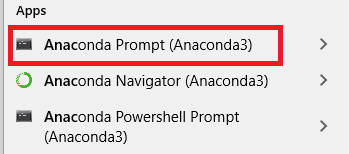
\includegraphics[width=.5\textwidth]{images/Chapter_02/AnacondaPrompt_Menu.png}
\end{center}

If you're on Linux, you only need to open a terminal. On Ubuntu, you can do this by pressing Ctrl+Alt+T. What's important to note is that when you trigger Anaconda, you'll see that your command line has a \mintinline{bash}{(base)} prepending it, as shown in the image below:

\begin{center}
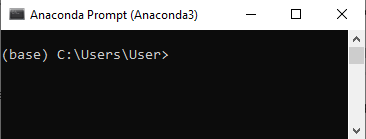
\includegraphics[width=.5\textwidth]{images/Chapter_02/AnacondaPrompt.png}
\end{center}

This is the best indication to know you're running the Anaconda installation. You can run the following command to see all the installed packages:

\begin{minted}{bash}
conda list
\end{minted}

The output you'll see will depend on what you have installed and whether or not you've already used Anaconda in the past. You'll see that at the beginning it tells you where your Anaconda installation is, followed by four columns: Name, Version, Build, and Channel. It should look something like this:

\begin{minted}{bash}
# packages in environment at /opt/anaconda3:
#
# Name                    Version                   Build  Channel
matplotlib                3.1.3                    py37_0
numpy                     1.18.1           py37h4f9e942_0
pyyaml                    5.3              py37h7b6447c_0
yaml                      0.1.7                had09818_2
\end{minted}

This image shows a few example packages, but your output should be much longer.

One of the good things about Anaconda is that it keeps track of each package, its version, and the build. The difference is that you may be using Anaconda on a computer with an Intel processor, or a Raspberry Pi with an ARM processor. In both cases, the version of, let's say, \py{numpy} may be the same, but they were compiled differently. You could also be using the same version of \py{numpy} but with a different version of Python (hence the \py{py37} that appears in the build numbers) which allows you to keep track of what you're doing at any given moment.

The last two lines show you a package called \py{pyyaml} that depends on a library called \py{yaml}, which you'll use later. With Anaconda, you can separately keep track of both the Python package and the lower-level library that this package uses. If you're coming from Linux, this won't be a great surprise, since this is precisely what the package manager on your computer does. If you're coming from Windows, however, this is something incredibly handy.

Say you want to install a package that you don't yet have on your machine. Let's see how you would install \py{PySerial}, which is a package that you'll use later in the book. Installing it becomes as easy as running the following command:

\begin{minted}{bash}
conda install pyserial
\end{minted}

This command outputs some information, such as the version and the build, then asks if you want to install it. You can select 'yes' and it will proceed. If you list the installed packages again, you'll notice that PySerial is listed there.

But this is not all Anaconda allows you to do. You can also use separate environments based on your projects.

\subsection{Working with Conda environments}\label{subsec:conda-environments}
A \textbf{conda environment} is, in practical matters, a folder where all the packages that you'll need to run your code are located, including any underlying libraries. the environments are \textbf{isolated} from each other; in other words, updating or deleting a package in one environment won't affect the state of that same package in any other environment. when you're working on different projects, there may be times where one needs a specific library version, and you don't want to ruin the other projects. to create a new environment, you need to run the following command (changing \py{myenv} to any name you want):

\begin{minted}{bash}
 conda create --name myenv
\end{minted}

then you activate it:

\begin{minted}{bash}
 conda activate myenv
\end{minted}

now if you list the installed packages you'll see there's nothing there:

\begin{minted}{bash}
conda list
# packages in environment at /opt/anaconda3/envs/myenv:
#
# name                    version                   build  channel
\end{minted}

from here, in your newly created environment, it's time to install the packages you want, starting with python itself:

\begin{minted}{bash}
 conda install python=3.7
\end{minted}

this will install the specified version of python in your new environment.

\infoInfo{Python Versions}{The \py{3.7} that you added after \py{python=} specifies which version of Python we want to use. If you don't specify it, then Anaconda installs the latest version, which at the time of writing is \py{3.8}. When Python updates, some libraries may not work correctly, or they  may not yet be available for that specific version. When selecting the Python version, be sure all your libraries are available.}

After installing Python, you can run it by typing:

\begin{minted}{bash}
 python
\end{minted}

The output will look something like this:

\begin{minted}{text}
Python 3.7.7 (default, Mar 26 2020, 15:48:22)
[GCC 7.3.0] :: Anaconda, Inc. on linux
Type "help", "copyright", "credits" or "license" for more information.
\end{minted}

To exit, just type:

\begin{minted}{bash}
exit()
\end{minted}

To follow the book, you'll need these packages:

\begin{itemize}
 \item NumPy -> For working with numerical arrays
 \item pySerial -> For communicating with serial devices
 \item PyYAML -> For working with YAML files, a specially structured text file
 \item PyQt -> For building Graphical User Interfaces
 \item PyQtGraph -> For plotting results within the User Interfaces
\end{itemize}

You can install all of these by running:

\begin{minted}{bash}
conda install numpy pyserial pyyaml pyqt pyqtgraph
\end{minted}

Don't worry too much about these packages, since you'll see them one-by-one later on.

If you run \mintinline{bash}{conda list}, you'll see that there are \emph{many} more packages installed. Each package depends either on other packages or libraries, and Anaconda took care of installing all of them for you. With a \mintinline{bash}{conda install} command, you can install packages that Anaconda itself maintains. These are official packages that come with a certification of quality. Many companies will allow their employees to only install packages that are officially supported by Anaconda, in order to avoid having malware installed within their network.

To follow the book, you'll need one more package called \py{Pint}. This package is \emph{not} in the official conda repositories. To install packages that aren't yet in the official repository, you can use an unofficial repository called \py{conda forge}. Packages that aren't mature enough, or versions that are too new and not tested enough, are located in this repository. To install a package, you just need to run the following command:

\begin{minted}{bash}
  conda install -c conda-forge pint
\end{minted}

The \mintinline{bash}{-c conda-forge} specifies the \py{channel} you want to install the package from. With this, you've finished installing all the packages you'll need to follow the rest of the book.

If you want to leave the environment, you can run:

\begin{minted}{bash}
conda deactivate
\end{minted}

This should return you to your normal shell prompt.

\subsubsection{Creating environments more quickly}
In the steps above, you created an empty environment and then installed the necessary packages. You can perform this operation slightly faster if you already know what you need. For example, you can do the following:

\begin{minted}{bash}
conda create --name env python=3.7 numpy=1.18 pyserial
\end{minted}

The command above creates an environment using the specified versions of Python and NumPy while using the latest version of PySerial.

\subsubsection{Removing an environment}
If you want to remove a conda environment called \py{env}, you can run the following command:

\begin{minted}{bash}
conda remove --name env --all
\end{minted}

\sloppy In practice, you also use the \py{remove} command to uninstall packages. When you do \py{remove --name env} it means that you want to remove a specific package from that environment, while the \py{--all} option tells Anaconda to remove \emph{all} the packages \emph{and} the environment itself. Use with care, since you can't undo it!

\section{Installing Pure Python}\label{sec:installing-pure-python}
If instead of Anaconda you prefer to install pure Python, the procedure is quite straightforward. It just varies slightly on different operating systems.

\subsection{Installing Python on Windows}\label{subsec:python-installation-on-windows}
Windows doesn't come with a pre-installed version of Python, so you'll need to install it yourself. Fortunately, it's not a complicated process. Go to the download page at Python.org, where you'll find a link to download the latest version of Python.

\tipsInfo{Note}{We've tested all the contents of this book with Python 3.7, but newer versions shouldn't give you any problems. If you install a more recent version and run into any problems later on, come back to this step, uninstall Python, and then reinstall an older version.}

Once the download is complete, you should launch the installer and follow the steps to install Python on your computer. Be sure that you select \textbf{Add Python 3.7 to the PATH}. If there are more users on the computer, you can also select \emph{Install Launcher} for all users. Just click on \textit{Install Now} and you're good to go! Pay attention to the messages that appear, just in case anything goes wrong.

\subsubsection{Testing your installation}
To test whether your installation of Python is working, you need to launch the Command Prompt, which is the Windows equivalent to a Terminal in most Unix operating systems. Throughout this book, we'll use the terms Command Prompt, Command Line, or Terminal interchangeably.

The Command Prompt is a program that allows you to interact with your computer by typing commands instead of using the mouse. To launch it, click the Start Button and search for \emph{Command Prompt} (it may be located in the Windows System apps). It should look like the image you see below:

\begin{center}
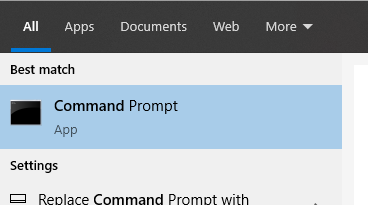
\includegraphics[width=.5\textwidth]{images/Chapter_02/CommandPrompt.png}
\end{center}

In the Command Prompt, you can do almost everything that you can do with the mouse on your computer. The command prompt starts in a specific folder on your computer, something similar to \mintinline{PowerShell}{C:\Users\User}. You can type \mintinline{bash}{dir} and press enter to get a list of all the files and folders within that directory. If you want to navigate through your computer, you can use the command \mintinline{bash}{cd}, which stands for \emph{change directory}. If you want to go one level up, then you can type \mintinline{bash}{cd ..}, where the two dots \mintinline{bash}{..} represent the parent folder of the one you're currently located in. If you want to enter a folder, then you type \mintinline{bash}{cd Folder} where \textit{Folder} is the name of the folder you want to change to.

It's out of the scope of this book to cover all the different possibilities that the Command Prompt offers you, but you shouldn't have any problems finding help online. See the image below to get an idea of what using the Command Prompt looks like on Windows:

\begin{center}
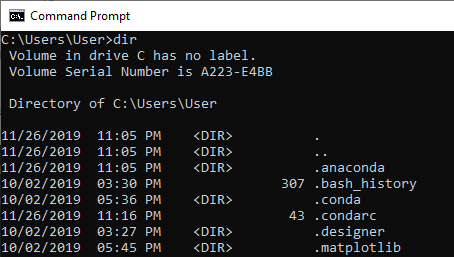
\includegraphics[width=.5\textwidth]{images/Chapter_02/CommandPrompt03.png}
\end{center}

To test that your Python installation was successful, just type \mintinline{bash}{python.exe} and hit enter. You should see a message like this:

\begin{minted}{powershell}
Python 3.7.7 (default, Oct  3 2017, 21:45:48)
[GCC 7.2.0] on Win64
Type "help", "copyright", "credits" or "license" for more information.
\end{minted}

The output shows you which Python version you're using as well as some extra information. You've just started what's called the Python Interpreter, which is an interactive way of using Python. If you come from a Matlab background, then you'll notice its similarities immediately. Go ahead and try it with some mathematical operation, like adding or dividing numbers:

\begin{minted}{pycon}
>>> 2+3
5
>>> 2/3
0.6666666666666666
\end{minted}

For future reference, when you see lines that start with \mintinline{pycon}{>>>} it means that you're working within the Python Interpreter. The lines without \mintinline{pycon}{>>>} in front are the output generated by the program.

\subsection{Adding Python to the PATH on Windows}\label{subsec:path-windows}
If you receive an error message saying that the command \mintinline{bash}{python.exe} was not found, then something went slightly wrong with the installation. Remember when you selected \textbf{Add Python to the PATH}? That option is what tells the Command Prompt where to find the program \mintinline{bash}{python.exe}. If, for some reason, it didn't work while installing, then you'll have to do this manually.

First, you need to find out where your Python is installed. If you paid attention during the installation process, then that shouldn't be a problem. Most likely you can find it in a directory like this one:

\begin{minted}{powershell}
C:\Users\**YOURUSER**\AppData\Local\Programs\Python\Python36
\end{minted}

Once you find the file \mintinline{bash}{python.exe}, copy the full path of that directory (that is, the location of the folder where you found \mintinline{bash}{python.exe}). You then have to add that file location to the system variable called PATH. Here are the steps you'll need to take:

\begin{enumerate}
    \item Open the System Control Panel. How to open it is slightly dependent on your Windows version, but it should be something like \emph{Start/Settings/Control Panel/System}.
    \item Open the \emph{Advanced} tab.
    \item Click the \emph{Environment Variables} button.
    \item Find the section called \emph{System Variables}. Select \emph{Path}, then click \emph{Edit}. You'll see a list of folders, each one separated from the next one by a semicolon (\py{;}).
    \item Add the folder where you found the \mintinline{bash}{python.exe} file at the end of the list. Don't forget the semicolon (\py{;}) to separate it from the previous entry.
    \item Click OK\@.
\end{enumerate}

You'll have to restart the Command Prompt for it to refresh the settings. Try to run \mintinline{bash}{python.exe} again and it should work.

\subsection{Installing Python on Linux}\label{subsec:installation-on-linux}
Most Linux distributions come with Python already installed. To check whether it's already on your system, open up a terminal (Ubuntu users can press Ctrl+Alt+T). You can then type \mintinline{bash}{python3}, and press enter. If it works you should see something like this appear on the screen:

\begin{minted}{bash}
Python 3.6.3 (default, Oct  3 2017, 21:45:48)
[GCC 7.2.0] on Linux
Type "help", "copyright", "credits" or "license" for more information.
\end{minted}

If it doesn't work, then you need to install Python 3 on your system. Ubuntu users can do this by running the following:
\begin{minted}{bash}
sudo apt install python3
\end{minted}

Each Linux distribution has a slightly different way of installing Python, but all of them more or less follow the same procedure. After the installation, check to see if it went well by typing \mintinline{bash}{python3} and hitting enter. Future releases of the operating system will include only Python 3 by default, and you won't need to add the \emph{3} explicitly. In case there's an error, try running only \mintinline{bash}{python} first and check whether your machine recognizes that you want to use Python 3.

\subsection{Installing Python packages}\label{subsec:installing-python-packages2}\label{subsec:installing-python-packages}
One of the characteristics that makes Python such a versatile programming language is the variety of packages that you can use in addition to the standard library. Python has a repository of applications called PyPI, which stands for the Python Package Index. PyPI contains more than one hundred thousand packages. The easiest way to install and manage these packages is through a command called \textbf{pip}. pip fetches the needed packages from the repository and installs them for you. pip is also capable of removing and upgrading packages. More importantly, pip handles dependencies so you don't have to worry about them.

pip works both with Python 3 and Python 2. To avoid mistakes, you have to be sure that you're using the version of pip that corresponds to the Python version you want to use. If you're on Linux and have both Python 2 and Python 3 installed, there are probably two commands, \py{pip2} and \py{pip3}. You should use the latter to install packages for Python 3. On Windows, you likely have to use \mintinline{PowerShell}{pip.exe} instead of just \mintinline{bash}{pip}. If this doesn't work for some reason, you'll need to follow the same procedure that you saw earlier to add \mintinline{bash}{python.exe} to the PATH, but this time with the location of your \mintinline{bash}{pip.exe} file.

\tipsInfo{Info}{Since the moment Anaconda was born up until now, pip has gone through many trials and tribulations. Today, you can install complex packages such as NumPy or PyQt directly. However, there's still some discussion regarding how much we can expect from pip at the moment as far as compiling programs or performing complex tasks.}

Now, installing a package becomes very simple. If you'd like to install a package such as NumPy, you should just type the following:
\begin{minted}{bash}
pip install numpy
\end{minted}

Windows users should type this:
\begin{minted}{powershell}
pip.exe install numpy
\end{minted}

\warningInfo{Before You Continue}{Before installing the packages listed below, it's essential that you read the following section on \textbf{Virtual Environments}. These will help you maintain clean and separate environments for software development.}

\begin{itemize}
 \item NumPy -> To work with numerical arrays
 \item Pint -> To use units and not just numbers
 \item pySerial -> To communicate with serial devices
 \item PyYAML -> To work with YAML files, a specially structured text file
 \item PyQt5 -> To build Graphical User Interfaces
 \item PyQtGraph -> To plot results within the User Interfaces
\end{itemize}

\sloppy You can install all the packages with pip without trouble. If you're in doubt, you can search for packages by typing \mintinline{bash}{pip search package_name}. Usually, the order in which you install the packages doesn't matter. Notice that since pip installs the dependencies, you sometimes get a message saying that a package is already installed, even if you didn't do it manually.

To build user interfaces, we've decided to use Qt Designer, an external program provided by the creators of Qt. You don't need to have this program installed to develop a graphical application because you can do everything directly from within Python itself. However, this approach can be much more time-consuming than dragging and dropping elements onto a window.

\subsection{Working with virtual environments}\label{subsec:virtual-environment2}
When you start developing software, it is of the utmost importance that you have an \textbf{isolated programming environment} to precisely control the packages that are installed. For example, you can use experimental libraries without overwriting software that other programs use on your computer. With virtual environments, you can update a package within that specific environment only, without altering the dependencies for any additional development you might be doing.

If you're working in a lab, then it's even more critical to isolate different environments. In essence, you're developing a program with a specific set of libraries, each with its own version and installation method. One day you or another researcher who works with the same setup might decide to try out a program that requires slightly different versions for some of the packages. The outcome can be a disaster: If there's an incompatibility between the new libraries and the computer software, then you could ruin the very program that controls your experiment!

Unintentional library upgrades can set you back several days. Sometimes it might be so long since you installed a library that you can no longer remember how to do it or where to get the same version you had. Other times you may want to check what would happen if you were to upgrade a library, or you might wish to reproduce the set of packages installed by a different user to troubleshoot any issues. There's no way of overestimating the benefits of isolating environments on your computer.

Fortunately, Python provides you with \textbf{virtual environments} that give you a lot of control and flexibility. A virtual environment is nothing more than a folder where you'll find copies of the Python executable and all the packages you installed. Once you activate the virtual environment, every time you trigger pip for installing a package, it will do so within that directory. The Python interpreter will be the one inside the virtual environment and not any other one. It may sound complicated, but in practice, it's incredibly simple.

You can create isolated working environments for developing software to run specific programs or for performing tests. If you need to update or downgrade a library, you'll do so within that specific virtual environment, and you won't alter the functioning of anything else on your computer. It may take some time for you to acknowledge the advantages of using virtual environments, but once you lose days or even weeks reinstalling packages because something went wrong and your experiment doesn't run anymore, you'll understand.

\criticalInfo{Warning}{Virtual environments are excellent for isolating Python packages, but many packages rely on libraries installed on the operating system itself. If you need a higher degree of isolation and reproducibility, you should check out Anaconda.}

\subsubsection{Working with virtual environments on Windows}
Windows doesn't have the most user-friendly command line, and some of the tools you can use for Python are slightly trickier to install than on Linux or Mac. The steps below will guide you through the installation and configuration of virtual environments on a Windows machine. If something is failing, then try to find help or examples online. There are a lot of great examples on StackOverflow, for instance.

Python comes bundled with a tool for creating virtual environments, so you can install the package with pip:

\begin{minted}{powershell}
pip.exe install virtualenv
pip.exe install virtualenvwrapper-win
\end{minted}

To create a new environment called \mintinline{bash}{Testing} you have to run the following:

\begin{minted}{powershell}
mkvirtualenv Testing --python=path\to\python\python.exe
\end{minted}

The last piece is crucial because it allows you to select the exact version of Python you want to run. If you have more than one version of Python installed, then you can choose whether you wish to use, for instance, Python 2 or Python 3 for that specific project. The command also creates a folder called Testing, where you'll find all the required packages and programs. If everything went well, then you should see that your command prompt now displays a \mintinline{bash}{(Testing)} message before the path. This means that you are indeed working inside the environment.

Once you've finished working on your project and you want to leave the virtual environment, you can type the following:

\begin{minted}{powershell}
deactivate
\end{minted}

This will return you to the normal command prompt. If you want to work on \mintinline{bash}{Testing} again, you have to type:

\begin{minted}{powershell}
workon Testing
\end{minted}

If you want to test that things are working fine, you can upgrade pip by running:

\begin{minted}{powershell}
pip install --upgrade pip
\end{minted}

If there's a new version available, then it will be installed. One of the most useful commands to run within a virtual environment is this:

\begin{minted}{powershell}
pip freeze
\end{minted}

This command gives you a list of all the packages installed within that working environment and their exact versions. This is so you'll know what you're using and can revert if anything goes wrong. Moreover, for people who are worried about the reproducibility of the results, keeping track of specific packages is a great way to be sure that you can repeat everything later.

You can install the packages listed before, such as NumPy and PyQt5, and see that they will only be installed within your \mintinline{bash}{Testing} environment. If you activate or deactivate the virtual environment, the packages you installed within it will not be available, which you can see with \mintinline{bash}{pip freeze}.

\subsubsection{Working with virtual environments in Windows PowerShell}
If you're using Windows PowerShell instead of the Command Prompt, there are some things that you have to change. First is the virtual environment wrapper package, which needs to be installed separately for PowerShell:

\begin{minted}{powershell}
pip install virtualenvwrapper-powershell
\end{minted}

Most likely, you'll need to change the execution policy of scripts on Windows. Open a PowerShell with administrative rights (to do so, right-click on the PowerShell icon and then select \emph{Run as Administrator}). Then run the following command:

\begin{minted}{powershell}
Set-ExecutionPolicy RemoteSigned
\end{minted}

Follow the instructions that appear on the screen to allow the changes on your computer. This should allow the wrapper to work. You can repeat the same commands that you saw before to create a virtual environment.

If it still doesn't work, don't worry too much. Sometimes there's a problem with the wrapper, but you can still create a virtual environment by running the following:

\begin{minted}{powershell}
virtualenv.exe Testing --python=path\to\python\python.exe
\end{minted}

This command creates the virtual environment within the Testing folder. Go to the folder Testing/Scripts and run:
\begin{minted}{powershell}
.\activate
\end{minted}

Now you're running within a virtual environment in PowerShell.

\subsubsection{Working with virtual environments on Linux}
Installing the virtual environment packages on Linux is more routine. Depending on where you installed Python, you may need root access to follow the installation. If you're unsure, first try to run the commands without \mintinline{bash}{sudo}, and if they fail, run them with \mintinline{bash}{sudo} as shown below:

\begin{minted}{bash}
sudo -H pip3 install virtualenv
sudo -H pip3 install virtualenvwrapper
\end{minted}

If you're on Ubuntu, you can install the package through apt, although it's not recommended:
\begin{minted}{bash}
sudo apt install python3-virtualenv
\end{minted}

To create a virtual environment, you need to know where to find the Python version you would like to use. The easiest way to do this is to note the output of the following command:

\begin{minted}{bash}
which python3
\end{minted}

The output will tell you the location of the program that's triggered when you run \mintinline{bash}{python3} in a terminal. Replace the location of Python in the following command:
\begin{minted}{bash}
mkvirtualenv Testing --python=/location/of/python3
\end{minted}

This creates a folder, usually \mintinline{bash}{~/.virtualenvs/Testing}, with a copy of the Python interpreter and all the packages that you need, including pip. That folder is your virtual environment and is the place where new modules will be installed. If everything went well, then you'll see the \mintinline{bash}{(Testing)} string at the beginning of the line in your terminal. When you see it, you know that you're working within a virtual environment.

To close the virtual environment you have to type the following:

\begin{minted}{bash}
deactivate
\end{minted}

To work in the virtual environment again, just do this:
\begin{minted}{bash}
workon Testing
\end{minted}

If for some reason the wrapper isn't working, you can create a virtual environment manually by executing the following code:
\begin{minted}{bash}
virtualenv Testing --python=/path/to/python3
\end{minted}
Then, you can activate it by executing the following command:
\begin{minted}{bash}
source Testing/bin/activate
\end{minted}

Bear in mind that in this way, you create the virtual environment wherever you are on your computer and not in the default folder. This behavior can be handy if, for example, you want to share the virtual environment with somebody, or place it in a precise location on your computer.

Once you've activated the virtual environment, you can install the packages listed before, such as NumPy. You can compare what happens when you're in the environment to what happens outside, and check that you truly are isolated from the central Python installation. The packages that you install inside of \mintinline{bash}{Testing} should not be available outside of it.

One of the most useful commands to run within a virtual environment is this:

\begin{minted}{bash}
pip freeze
\end{minted}

This command gives you a list of all the packages installed within that working environment and their exact versions. This is so you'll know what you're using and can revert the package version if anything goes wrong. Moreover, for people who are worried about the reproducibility of the results, keeping track of specific packages is a great way to be sure that anyone can repeat the results at a later time.

\section{Using Qt Designer}\label{sec:install-qt-designer}
Qt Designer is a great tool to quickly build user interfaces by dragging and dropping elements onto a canvas. It allows you to swiftly develop elaborate windows and dialogs, styling them and defining some basic features without writing actual code. We use this program to design a detailed window in which the user can tune the experiment parameters and display data in real-time.

If you're using \textbf{Anaconda}, the Designer comes already bundled with it, so you don't need to follow the steps below.

\subsection{Installing Qt Designer on Windows}\label{subsec:installing-on-windows}
Installing Qt Designer on Windows only takes one Python package: \mintinline{bash}{pyqt5-tools}. Run the following command:

\begin{minted}{bash}
pip install pyqt5-tools
\end{minted}

\sloppy The designer should be located in a folder called \mintinline{bash}{pyqt5-tools}. The folder's location depends on how you installed Python and whether you're using a virtual environment. If you aren't sure, then use the tool to find folders and files in your computer and search for \mintinline{bash}{designer.exe}.

\tipsInfo{Info}{The package \mintinline{bash}{pyqt5-tools} is an independent package aimed at making the installation of the Qt Designer easier. However, it takes a bit of time for it to update to the latest version of Python. At the time of this writing, it's known to work with Python 3.8, but not with Python 3.9.}

\subsection{Installing Qt Designer on Linux}\label{subsec:installing-on-linux}
Linux users can install Qt Designer directly from within the terminal by running the following command:

\begin{minted}{bash}
sudo apt install qttools5-dev-tools
\end{minted}

To start the Designer, just look for it within your installed programs, or type \mintinline{bash}{designer} and press enter in a terminal.

\section{Choosing a Text Editor}\label{sec:editors}
To complete the Python For The Lab book, you'll need a \textbf{text editor}. As with many decisions in this book, you are entirely free to choose whichever one you like. Still, there are some resources we'll point out that can be useful to you.

You won't need anything more sophisticated for editing code than a \textbf{plaintext editor}, such as Notepad++. This is available on Windows only, and it's very basic and straightforward. You can have several tabs open with different files and you can perform a search for a specific string in your opened documents, or even within an entire folder. Notepad++ is very good for small changes to code, perhaps made directly in the lab. The equivalent to Notepad++ on Linux are text editors such as Gedit or Kate. Every Linux distribution comes with a pre-installed text editor.

Developing software for the lab requires working with different files simultaneously, being able to check that your code is correct before running it, and ideally being able to interface directly with virtual environments (whether you're using conda or virtualenv). For all this, there is a range of programs called IDEs or \textbf{Integrated Development Environments}. We strongly suggest you check out \textbf{PyCharm}, which offers a free and open-source Community Edition as well as a Professional Edition (which you can get for free if you're a student or teacher affiliated with a university). PyCharm integrates itself with virtual environments and allows you to install a package if it's missing, but you need it and many more things. It's a sophisticated program, but there are many great tutorials on how to get started. Familiarizing yourself with PyCharm pays off quickly.

Another very powerful IDE for Python is \textbf{Microsoft's Visual Studio Code}, which is very similar to PyCharm in it's capabilities. If you have previous experience with Visual Studio, I strongly suggest you keep using it. It integrates very nicely with your workflow. Visual Studio is available not only for Windows but also for Linux and Mac. It has some excellent features for inspecting elements and helping you debug your code. The community edition is free of charge. Support for Python is complete, and Microsoft has released several video tutorials showing you how to get the best out of their program.

There are other options around, such as Atom or Sublime. However, they don't specifically target Python as the previous two do. Remember that the choice is always yours. Editors should be a tool and not an obstacle. If you've never used an IDE before, then we recommend you just go ahead and install PyCharm. That's what we use during the workshops, and everyone has always been very pleased with it. If you already have an IDE or a workflow with which you are happy, then keep it! If at some point it starts failing you, then you can reevaluate the situation.

\warningInfo{Tabs or Spaces}{Python is sensitive to the use of \textbf{tabs} and \textbf{spaces}. You shouldn't mix them! A good standard is to use four spaces to indent your code. If you decide to go for a text editor, then be sure to configure it to respect Python's stylistic choices. Notably, Notepad++ comes preset to use tabs instead of spaces, which is a problem if you ever copy and paste code from other sources.}

    \chapter{Writing the First Driver}\label{ch:first-driver}

\section{Objectives}\label{sec:driver-objectives}
Communicating with real-world devices is the cornerstone of every experiment. However, devices are very different from each other. Not only is their behavior different (you can't compare a camera to an oscilloscope), but they also communicate in different ways with the computer. In this chapter,
we are going to build the first driver for communicating with a real-world device. You are going to learn about low-level communication with a serial device and, from that experience, build a reusable class that you can share with other developers.

\section{Introduction}\label{sec:driver-introduction}
We can split devices into different categories depending on how they communicate with a computer. One of the most common ways to communicate is through the exchange of text messages. The idea is that the user sends a specific command, i.e., a message, and the device answers with specific information, another message. Sometimes there is no answer because it is just a command to perform an action such as an auto setting or switching off. Sometimes the message we get back contains the information we requested.

To have an idea of how commands look like, you can check the manuals of devices such as oscilloscopes or function generators. Both Tektronics\footnote{You can check the manual of an oscilloscope here: https://www.tek.com/oscilloscope/tds1000-manual} and Agilent have complete sets of instructions. If you search through their websites, you find plenty of examples. A command that you can send to a device may look like this:

\begin{minted}{text}
 *IDN?
\end{minted}

Which is asking the device to identify itself. An answer to that request would look like \texttt{Oscilloscope ID\#\#\#\#\#\#}. In this chapter, we are going to see how you can exchange messages with devices using Python.

The devices that exchange information with the computer in this way are called \textbf{message-based} devices. Some of this type of device are oscilloscopes, lasers, function generators, lock-ins, and many more. The {PFTL DAQ} device to work with this book also enters into this category. If you got the book online and not as part of a workshop, you can build your device or contact us, and we may be able to offer you one already programmed\footnote{courses@pythonforthelab.com}.

\note{There is an entire world of devices that do not communicate through messages, such as cameras, fast data acquisition cards, motorized mirrors and stages, and more. They depend on specific drivers and are harder to work with at this stage. If you are already confident programming message-based devices and need to move to non-message based ones, you can check the Advanced Python for the Lab materials.}

Remember, \textit{message-based} refers only to how the device exchanges information with the computer, and not to the actual connection between them. It is possible to connect a message-based device via RS-232, USB, GPIB, or TCP/IP. Be aware, however, that it is not a reciprocal relation: not all devices connected through RS-232 or USB are message-based. If you want to be sure, check the manual of the device and see how it is controlled. In this chapter, we are going to build a driver for a message based device.

\subsection{Scope of the Chapter}\label{subsec:scope-of-the-chapter}
In the introduction, we discussed that the objective is to acquire the I-V curve of a diode. You need, therefore, to set an analog output (the V) and read an analog input (the I) with the device. In this chapter, we focus
on everything we need to perform our first measurement. However, keep in mind the onion principle, which tells you that you should always be prepared to expand your code later on if the need arises.

\section{Communicating with the Device}\label{sec:message-basedevices}
To communicate with the {PFTL DAQ}\footnote{PFTL is the shorthand notation for Python For the Lab} device, we are going to use a package called \texttt{PySerial}, which you should have already installed if you followed chapter~\ref{ch:setting-up}. The first thing we can do is to list all the devices connected to the computer to identify the one in which we are interested. Plug your device via the USB port of your computer. We need to connect the {PFTL DAQ} device through the micro USB port closest to the power jack, also known as \emph{programming port}. Then, the following command in a terminal (be sure you are within the environment in which you have installed the required packages):

\begin{minted}{bash}
python -m serial.tools.list_ports
\end{minted}

\note{From now on, instead of telling you to open a terminal to run a command, if you see code which starts with a \texttt{\$} symbol, it means that you should run it in the terminal}

Depending on the operating system, the output can be slightly different. On Windows, we get something like this:

\begin{minted}{bash}
COM3
\end{minted}

While if you are on Linux you will see something like this:

\begin{minted}{bash}
/dev/ttyACM0
\end{minted}

The most important thing is to remember the number at the end. If you happen to see more than one device listed (this is very common on Mac), unplug the {PFTL DAQ}, run the command to list the ports again, note which ones appear. Plug it back and list the devices. The new one is the device in which we are interested.

Now is time to start working with the device. Start Python by running:

\begin{minted}{bash}
$ python
\end{minted}

And then we can start working directly from the command line. First, we are going to import the package we need for communication:

\begin{minted}{pycon}
>>> import serial
\end{minted}

\note{Earlier we explained that we must run in a terminal everything prepended with a \$. Lines prepended by \texttt{>>>} are lines that run in a Python interpreter. Note that there is no need to type the \texttt{>>>}}

And then we can open the communication with the device. Bear in mind that you must change the port number by the one you got earlier:

\begin{minted}{pycon}
>>> device = serial.Serial('/dev/ttyACM0') # <---- CHANGE THE PORT!
\end{minted}

Now we are ready to get started exchanging messages with the device. Before we discuss each line, let's see what you can do. The lines without \texttt{>>>} are the output generated by the code.

\begin{minted}{pycon}
>>> device.write(b'IDN\n')
4
>>> answer = device.readline()
>>> print(f'The answer is: {answer}')
The answer is: b'PFTL DAQ Device built by Python for the Lab v.1.2020\n'
>>> device.close()
\end{minted}

Even if short, many things are going on in the code above. First, we import the \texttt{PySerial} package, noting that we are actually importing \texttt{serial} and not \texttt{PySerial}. Then we open the specific serial port that identifies the device. Bear in mind that serial devices can maintain only one connection at a time. If you try to run the line twice, it gives you an error letting you know that the device is busy. It happens if, for example, we try to run two programs at the same time, or if we start Python from two different terminals.

Once we established the connection, we send the \textbf{{IDN}} command to the device. There are some caveats in the process. First, the \mintinline{python}{\n} at the end, is a special character known as \texttt{newline}. It is a way to tell the device that we are
not going to send more information afterward. When a device is receiving a command, it reads the input until it knows that no more data is arriving. If we were sending a value to a device such as a wavelength, the command could look like \texttt{SET:WL:1200}. However, the device needs to know when it has received the last number. It is not the same setting the laser wavelength to $120\,\textrm{nm}$ or to $1200\,\textrm{nm}$.

The other particular detail is the \mintinline{python}{b} before the command string. Adding the \mintinline{python}{b} in front of a string is one way of telling Python to encode a string as a binary string. Devices don't understand what an \textit{A} is. The serial communication can only send a stream of 1's and 0's. Therefore, we need to transform any information we are trying to send, such as \mintinline{python}{'IDN'}, to bytes before we can send it to the device. We give a lengthier discussion about encoding strings and what it means at the end of the chapter, in section \ref{section:unicode}.

After we write to the device, we get a \texttt{4} as output. It is the number of bytes we sent, taking into account that \mintinline{python}{\n} is only one byte because it is only one character. To get the answer that the device is generating for us, we have to read from it. We use the method \mintinline{python}{readline()} for this. Then we print the answer to the screen. The answer we get also has a \texttt{\\n} and a \texttt{b}. Finally, we close the connection to the device.

We decided to use the \texttt{IDN} command because we knew it existed. But if we are starting with a new device, it is always fundamental to start by reading the manual. Manuals are our best and, perhaps, the only friend we have when developing software for controlling instruments. The {PFTL DAQ} is no exception. The manual is part of the book, and we can find it in chapter \ref{chapter:pftl-daq-manual}. It is a simple manual, but with enough information to get started, and it follows similar conventions to those we can find on more complex devices.

In the manual, the first thing we have to find is the line termination. We used the newline character because we knew it, but each device can specify something different. Some devices use the newline character as part of the commands you can send and specify that the line ending must be something else. Once we know how to terminate commands, we can go ahead and see the list of options.

Many devices (but not all) follow a standard called \href{https://en.wikipedia.org/wiki/Standard_Commands_for_Programmable_Instruments}{SCPI}. The standard makes devices easy to exchange, because the commands for all oscilloscopes are the same, for all function generators are the same, and so forth. Moreover, the SCPI standard follows a structure that makes messages easy to understand and modular. A more powerful oscilloscope, for example, has commands not available to a more basic device, but the common features are controlled by the same messages.

Now that we know how to get started with serial communication, it is time to move to more complex programs. Typing everything on the Python interpreter is not handy and takes much time. So now we can start working with files.

\subsection{Organizing Files and Folders}
When we start a new project, it is always a good idea to decide how we are going to organize the work. In the previous chapter, we have set up an environment for developing a program. That is the first step to be organized. The second step is deciding where we are going to save the files we need to write our program. The general advice is to have a folder for all the programs, for example, \texttt{Programs}. Inside, each project we work on has its folder, such as \texttt{PythonForTheLab}. Each person has their way of organizing themselves, but from now on, every time we talk about creating a file, we are referring to that base folder for the project.

\section{Basic Python Script}
The code we have developed above can also be written as a Python script, that we can run from the command line without the need to re-write everything. Create an empty file called \textbf{communicate\_with\_device.py}, and add the same code we had earlier to it:

\begin{minted}{python}
import serial

device = serial.Serial('/dev/ttyACM0')
device.write(b'IDN\n')

answer = device.readline()
print(f'The answer is: {answer}')

device.close()
\end{minted}

Now we can run the file:

\begin{minted}{bash}
$ python communicate_with_device.py
\end{minted}

\note{To be able to run the file, you need to be in the same folder where the file is. To change the folder in the terminal, you can use \texttt{cd}}

\textbf{What happens when you run the file?}

The program hangs, there is no error message and no IDN information printed to the screen. It means the program is waiting for something to let it continue. To force the stop of the program, you can press Ctrl+C, and if this does not work on Windows, you can press Ctrl+Pause/Break. Now can see the easiest way to debug when such a situation appears.

We want to know first when the program hangs, and then we can see how to fix it. So we can edit the file and add some print statements to check until which point is running:

\begin{minted}{python}
import serial
print('Imported Serial')

device = serial.Serial('/dev/ttyACM0')
print('Opened Serial')

device.write(b'IDN\n')
print('Wrote command IDN')

answer = device.readline()
print(f'The answer is: {answer}')

device.close()
print('Device closed')
\end{minted}

Rerun the script. \textbf{Where is it hanging?} Surprisingly, it is hanging during the \texttt{readline} execution. Can you understand what is going on?

There is something very different between writing on the Python interpreter and running a script: the time it takes to go from one line to the other. While you type, everything happens slowly, while when you run a script, everything happens incredibly fast. Now, the \texttt{readline} is waiting to get some information from the device, but the devices are not generating it. It means that the problem should be earlier when we sent the \texttt{IDN} message. The command is not wrong in itself, but what is happening is that between opening the communication with the device and sending the first message, we give no space.

When you establish communication with most devices, there is a small delay until you can start using it. In our case, we must add a delay between starting the communication and sending the first message. We can achieve this by doing the following:

\begin{minted}{python}
import serial
from time import sleep

device = serial.Serial('/dev/ttyACM0')
sleep(1)

device.write(b'IDN\n')
answer = device.readline()
print(f'The answer is: {answer}')
device.close()
print('Device closed')
\end{minted}

If you rerun the program, you can see that it takes a bit of time to run, but it outputs the proper message. The \texttt{sleep} function makes the program wait for a given number of seconds (also fractions) before continuing. You can try lowering the number until you get the minimum possible value. Still, in typical cases, you start the communication only once, therefore waiting 1 second or .5 seconds won't have a significant impact on the overall execution time.

\subsubsection{Reading an Analog Value}
Before we continue, it would be great to also read a value from the device, not just the serial number. If we refer again to the manual, we see that the way of getting an analog value is using the \texttt{IN} command. We can modify the code on our previous program to read a value with the device:

\begin{minted}{python}
import serial
from time import sleep

device = serial.Serial('/dev/ttyACM0')
sleep(1)

device.write(b'IDN\n')
answer = device.readline()
print(f'The answer is: {answer}')

device.write(b'IN:CH0\n')
value = device.readline()
print(f'The value is: {value}')
device.close()
print('Device closed')
\end{minted}

The value you are reading doesn't make much sense, especially if there is nothing connected to the input number 0; it is just noise. But it is an excellent first step. We can acquire a value from the real world using the device. We take care of all the things that we need to address in the following chapters.

\exercise{What happens if you use \mintinline{python}{read()} instead of \mintinline{python}{readline()}?}

\exercise{What happens if you use \texttt{read()} once, and then \texttt{readline()}?}

\exercise{What happens if you call \texttt{readline()} before writing the \texttt{IDN} command?}

\exercise{What happens if you try to write to the device after you have closed it?}


\note{\textbf{Important note about ports}: If you are using the old {RS}-232 (also simply known as \emph{serial}), the number refers to the physical number of the connection, on Windows, it is something like {COM1}, on Linux and Mac, it is something like /dev/ttyACM1. In modern computers, there are no {RS-232} connections, and most likely, we have to use a {USB} hub for them. It means that there is no physical connection
straight from the device into the motherboard. The numbering can change if we plug/unplug the cables. The {PFTL DAQ} device, since it acts as a hub for a serial connection, can show the same behavior. If you plug/unplug the device while it is being used, the port we get the second time is likely different. The second time we run the program, we need to update the information.}

\exercise{Read the manual of the {PFTL DAQ} and find a way to set an analog output to 1 Volt.}

\section{Preparing the Experiment}
Before moving forward with programming, it is time to set up the measurement we want to perform and discuss what we need to achieve it. This book revolves around the idea of measuring the I-V curve of a diode. If you are not too familiar with electronics, don't worry, it is not essential to follow the book, you can just copy the connections as shown below. If you are a bit more familiar with electronics, it is worth explaining what we are going to do.

Diodes are elements that let current flow only in one direction, but their behavior is highly non-linear. The current flowing is not proportional to the voltage applied. We chose to use an LED for the experiments because it is easy to have visual feedback on what is going on. On the other hand, we can't measure current directly. First, we need to transform it into a voltage. If you are familiar with Ohm's law, you remember the relationship:

\begin{equation}
V = I \cdot R
\end{equation}

Voltage is current times resistance. Therefore, if we want to transform a current to a voltage, we just need to add a resistance to the circuit.

To perform the experiment, we need to apply a given voltage and read a  voltage. This pattern is common to a wealth of experiments. The underlying meaning is what matters.

With the {PFTL DAQ} device, the connections that will allow us to apply a voltage and read a voltage are as follows:

\begin{figure}
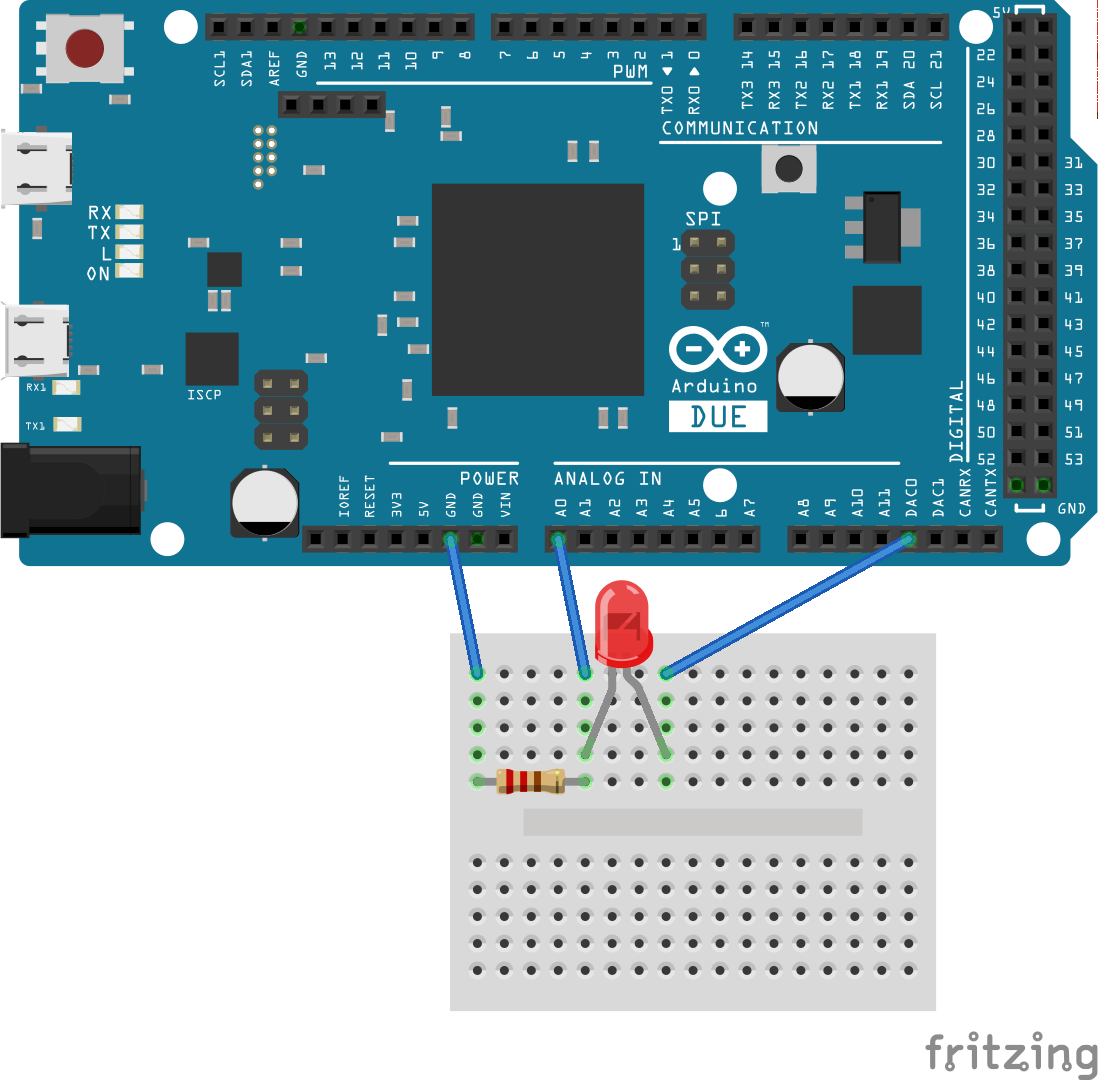
\includegraphics[width=.5\textwidth]{images/Chapter_03/IV_scheme_bb.png}
\caption{Schematic of the connections to perform the experiment}
\end{figure}

Only three cables, an LED and a resistance, are all you need to follow the rest of the book. We apply the voltage to the LED through \texttt{DAC0}. The current flows through the diode and the resistance. The voltage that we acquire at the Analog In \texttt{A0} is proportional to the current flowing through the resistance.

\exercise{Now that you have set up the experiment know how to set and read values. Acquire the I-V curve of the diode. It is a challenging exercise, aimed at showing you that it doesn't take a long time to be able to achieve an essential goal.}

\section{Going Higher Level}\label{section:going-higher-level}
We saw that communicating with a device implies taking into account parameters such as the line ending, or adding the \texttt{b} in front of messages for encoding. If the number of commands is large, it becomes very unhandy. The {PFTL DAQ} device is an exception because it is minimal, but there are still a lot of possible improvements.

If you still remember the \emph{Onion Principle} (section \ref{section:onion-principle}), it is now the time to start applying it. If you completed the last exercise, you probably have written much code to do the measurement. Perhaps you used a for loop, and acquired values in a sequence. However, if you want to change any of the parameters, you need to alter the code itself. This approach is not very sustainable for the future, especially if you are going to share the code with someone else.

Since we know how to communicate with the device, we can transform that knowledge into a reusable Python code by defining a class. Classes have the advantage of being easy to import into other projects, which are easy to document and to understand. Moreover, they are easy to expand later on. If you are not familiar with what classes are, check the appendix \ref{chapter:classes-in-python} for a quick overview. With a bit of patience and critical thinking, you can follow the rest of the chapter and understand what is going on as you keep reading.

Create a new, empty file, called \textbf{pftl\_daq.py}, and write the following into it:

\begin{minted}{python}
import serial
from time import sleep


class Device:
    def __init__(self, port):
        self.rsc = serial.Serial(port)
        sleep(1)

    def idn(self):
        self.rsc.write(b'IDN\n')
        return self.rsc.readline()

\end{minted}

The code above shows you how to start a class for communicating with a device and get its serial number. However, if you run the file, nothing happens. At the end of the file, add the following code:

\begin{minted}{python}
dev = Device('/dev/ttyACM0') #<---- Remember to change the port
serial_number = dev.idn()
print(f'The device serial number is: {serial_number}')
\end{minted}

If we rerun the code, we get the serial number of the device. Let's go line by line to understand what is going on. First, we create a class, and we define what do we want to happen when we do \texttt{Device()}. In the \texttt{\_\_init\_\_} method, we specify that the class needs a port, and we use that port to start the serial communication. The serial communication is stored as \texttt{self.rsc} in the class itself, where \texttt{rsc} is just a shorthand notation for \textit{resource}. Then we sleep for one second to give time to the communication to be established.

The second method, \texttt{idn}, just repeats what we have done earlier: we write a command, we read the line and return the output. If we look at the few lines at the bottom of the file, we now see that way of working with this class is simpler. We just use \texttt{idn()} instead of having to write and read every time.

\exercise{Once you read the serial number from the device, it does not change. Instead of just returning the value to the user, store it in the class in an attribute \mintinline{python}{self.serial_number}.}

\exercise{When you use the method \mintinline{python}{idn}, instead of writing to the device, check if the command was already used and return the value stored. This behavior is called caching, and is very useful not to overflow your devices with useless requests for data.}

\subsubsection{Reading and Setting Values}
We have just developed the most basic class, one that allows us to start the communication with the device and read its identification number. We can also write methods for reading an analog input or generating an output. The most important thing is to decide what argument each method needs. For example, reading a value only needs the channel that we want to read. Setting a value needs not only a channel but also the value itself. Also, reading a means that the method returns something. When you set an output, there is not much to return to the user.

\exercise{Write a method \mintinline{python}{get_analog_input} which takes two arguments: \mintinline{python}{self} and \mintinline{python}{channel} and which returns the value read from the specified channel.}

\exercise{Write a method \mintinline{python}{set_analog_value} which takes three  arguments: \mintinline{python}{self}, \mintinline{python}{channel} and \mintinline{python}{value} and that sets the output value to the specified port.}

Even though the exercises are important for you to start thinking by yourself, they have some caveats that are very hard to iron out if you don't have a bit of experience. First, let's look at the way of reading an analog input. We can try to develop a method that looks like this:

\begin{minted}{python}
def get_analog_input(self, channel):
    message = f'IN:CH{channel}\n'
    self.rsc.write(message)
    return self.rsc.readline()
\end{minted}

But it won't work, because even though we are adding the line ending, we are missing the \texttt{b} that we were using in the other examples. On the other hand, if we try to do something like:

\begin{minted}{python}
message = b'IN:CH{}\n'.format(channel)
\end{minted}

It will fail, because \texttt{format} only works with strings, and as soon as the \texttt{b} is added in front of a string, it is encoded to bytes. This means that we have to do it in two steps:

\begin{minted}{python}
def get_analog_input(self, channel):
    message = f'IN:CH{channel}\n'
    message = message.encode('ascii')
    self.rsc.write(message)
    return self.rsc.readline()
\end{minted}

First we form the message we want to send to the device, then we \emph{encode} it, which is the same as adding the \texttt{b} in front of a string. And then we write it to the device. After writing, we return the line with the value. We could use it as follows:

\begin{minted}{python}
dev = Device('/dev/ttyACM0') #<---- Remember to change the port
serial_number = dev.idn()
print(f'The device serial number is: {serial_number}')
volts = dev.get_analog_input(0)
print(volts)
\end{minted}

If you run the code anove, you will notice that the output still has the \texttt{b} and the \texttt{\\n}, we will work on this later. The next step is to generate an output:

\begin{minted}{python}
def set_analog_output(self, channel, output_value):
    message = f'OUT:CH{channel}:{output_value}\n'
    message = message.encode('ascii')
    self.rsc.write(message)
\end{minted}

And we can use it as follows:

\begin{minted}{python}
dev = Device('/dev/ttyACM0') #<---- Remember to change the port
serial_number = dev.idn()
print(f'The device serial number is: {serial_number}')
volts = dev.get_analog_input(0)
print(volts)
dev.set_analog_output(0, 1000)
\end{minted}

This would be all, unless we do add something extra, like reading the input after setting the output:

\begin{minted}{python}
dev = Device('/dev/ttyACM0') #<---- Remember to change the port
serial_number = dev.idn()
print(f'The device serial number is: {serial_number}')
volts = dev.get_analog_input(0)
print(volts)
dev.set_analog_output(0, 1000)
volts = dev.get_analog_input(0)
print(volts)
\end{minted}

The second time we read the analog input, we get the same value we passed to the analog output. It does not matter if it is $1000$ or $999$; it does not matter if the cables are connected or not. The value is always the same.

\exercise{Explain why when getting the analog input we get the same value that we set earlier}

This question is very tricky and requires that we read the manual of the device. In the documentation for the \texttt{OUT} command, you can see that it returns something: the same value that was passed to it. However, in our method, we are just writing to the device and not reading from it. The message waits in the queue until next time we read from it, and this happens when we try to read an analog input.

As you can see, the number of possible mistakes that we can do when developing this kind of programs is huge. On top of that, many mistakes do not generate an error, and can easily go unnoticed. When performing measurements, perhaps you don't realize the mistake on the \texttt{set\_analog\_output} until you are analyzing the data you acquired.

To solve the problem while setting the output, we just need to read from the device after setting the output:

\begin{minted}{python}
def set_analog_output(self, channel, output_value):
    message = f'OUT:CH{channel}:{output_value}\n'
    message = message.encode('ascii')
    self.rsc.write(message)
    self.rsc.readline()
\end{minted}

We are not doing anything with the information we get. We just clear it from the device.

\subsubsection{Proper Values Instead of Bytes}
To have a bit more functional class, it would be great if we could get rid of the extra \texttt{b} and \texttt{\\n} that we get every time we use the \texttt{readline()} function. First, we need to transform bytes to strings. In the previous section we transformed strings to bytes by using \texttt{.encode('ascii')}, and to no surprise, if we want to transform bytes to a string, we can do the opposite, in the \texttt{idn} method, for example:

\begin{minted}{python}
def idn(self):
    self.rsc.write(b'IDN\n')
    answer = self.rsc.readline()
    answer = answer.decode('ascii')
    return answer
\end{minted}

If you try this out, you will see that it took care of the initial \texttt{b}, but the \texttt{\\n} is still there. We need one more step to get rid of it:

\begin{minted}{python}
def idn(self):
    [...]
    answer = answer.strip()
    return answer
\end{minted}

Note that we have used \texttt{[...]} to hide the code that didn't change. Now you can go ahead and see that the output is formatted correctly.

\exercise{By using what you've learned for the \texttt{idn} method, improve the \texttt{get\_analog\_input} method so that it returns an integer. \textbf{Hint:} To transform a string to an integer, you can use \texttt{int()}, for example: \texttt{int(\'12\')}.}

\subsection{Abstracting Repetitive Patterns}
When you start to develop programs, there is a principle called \textbf{DRY}, which stands for \emph{don't repeat yourself}. Sometimes it is clear that code is repeating itself, for example, if we copy-pasted some lines. Sometimes, however, the repetition is not about code itself but a pattern. {DRY} is not a matter of just typing fewer lines of code. It is a way of reducing errors and making the code more maintainable. Imagine that after an upgrade, the device requires a different line ending. We would need to go through all your code to find out where the line ending is used and change it. If we would specify the line ending in only one location, changing it would require just to change one line.

First, we can specify the default parameters for our device. They will be all the constants that we need in order to communicate with it, such as line endings. We can define them just before the \mintinline{python}{__init__} method, like this:

\begin{minted}{python}
class Device:
    DEFAULTS = {'write_termination': '\n',
                'read_termination': '\n',
                'encoding': 'ascii',
                'baudrate': 9600,
                'read_timeout': 1,
                'write_timeout': 1,
                }
    def __init__(self, port):
        [...]
\end{minted}

You can see that there is much new information in the class. We have established a clear place where both the read and write line endings are specified (in principle they don't need to be the same), we also specify that we want to use ascii to encode the strings and that the baud rate is 9600. This value is the default of PySerial, but it is worth making it explicit in case newer devices need a different option. We also specify timeouts, which are allowed by PySerial and would prevent the program from freezing if writing or reading takes too long.

It is normally good practice to separate the instantiation of the class with the initialization of the communication. One thing is creating an object in Python, and the other is to establish communication with a real device. Therefore, we can rewrite the class like this:

\begin{minted}{python}
def __init__(self, port):
    self.port = port
    self.rsc = None

def initialize(self):
    self.rsc = serial.Serial(port=self.port,
                        baudrate=self.DEFAULTS['baudrate'],
                        timeout=self.DEFAULTS['read_timeout'],
                        write_timeout=self.DEFAULTS['write_timeout'])
    sleep(1)
\end{minted}

You can see that there are some major changes to the code, but the arguments of the \mintinline{python}{__init__} method are the same. In this way, code already written does not fail if we change the number of arguments of a method. When we do this kind of change, it is called \emph{refactoring}. It is a complex topic, but one of the best strategies you can adopt is not to change the number of arguments functions take, and the output should remain the same. In the class, the \mintinline{python}{__init__} definition looks the same, but its behavior is different. Now, it just stores the \mintinline{python}{port} as the attribute \mintinline{python}{self.port}. Therefore, to start the communication with the device, we need to do \mintinline{python}{dev.initialize()}. You can also see that we have used almost all the settings from the \mintinline{python}{DEFAULTS} dictionary to start the serial communication.

After we do these changes, we should also update the code we use to test the device:

\begin{minted}{python}
dev = Device('/dev/ttyACM0') #<---- Remember to change the port
dev.initialize()
serial_number = dev.idn()
print(f'The device serial number is: {serial_number}')
volts = dev.get_analog_input(0)
print(volts)
dev.set_analog_output(0, 1000)
volts = dev.get_analog_input(0)
print(volts)
\end{minted}

So far the only difference with the previous code is the \mintinline{python}{__init__} method. We have to improve the rest of the class. We already know that for message-based devices there are two operations: \textbf{read} and \textbf{write}. However, we will only read after a write (remember, we should ask something from the device first.) It is possible to update the methods of the class to reflect this behavior. Since all the commands of the device return a value, we can develop a method called \texttt{query}:

\begin{minted}{python}
def query(self, message):
    message = message + self.DEFAULTS['write_termination']
    message = message.encode(self.DEFAULTS['encoding'])
    self.rsc.write(message)
    ans = self.rsc.readline()
    ans = ans.decode(self.DEFAULTS['encoding']).strip()
    return ans
\end{minted}

In this way, we take the message, append the proper termination, and encodes it as specified in the \texttt{DEFAULTS}. Then, it writes the message to the
device exactly as we did before. Then we read the line, we decode it using the defaults and strip the line ending. Now it is time to update the other methods of the class to use the \texttt{query} method we have just developed. Let's start with \texttt{idn}, which now looks like this:

\begin{minted}{python}
def idn(self):
    return self.query('IDN')
\end{minted}

And the same we can do for the other methods:

\begin{minted}{python}
def get_analog_input(self, channel):
    message = 'IN:CH{}'.format(channel)
    ans = self.query(message)
    ans = int(ans)
    return ans

def set_analog_output(self, channel, output_value):
    message = 'OUT:CH{}:{}'.format(channel, output_value)
    self.query(message)
\end{minted}

For such a simple device, perhaps the advantages of abstracting patterns are not evident. It is something that happens very often in more extensive programs, and being able to identify those patterns can make the difference between a successful program and something only one person can understand. Note that even if we have changed the methods for identifying, reading, and setting analog values, there is no need to update the example code.

It is important to see that we achieved the communication with the device through the resource \mintinline{python}{self.rsc} that is created with the method \mintinline{python}{initialize}. There is a common pitfall with this command. If we try to interact with the device before we initialize it, we get an error like the following:

\begin{minted}{python}
AttributeError: 'NoneType' object has no attribute 'write'
\end{minted}

We now remember why this happened, but it is very likely that in the future, either we forget or someone else is using our code, and the error message that appears is incredibly cryptical. Therefore, we suggest you do the following:

\exercise{Improve the \texttt{query} method to check whether the communication with the device has initialized. If it hasn't, you can print a message to the screen and prevent the rest of the program from running.}

When we develop code, we must always keep an eye on two people: the future us and other users. It may seem obvious now that we initialize the communication before attempting anything with the device, but in a month, or a year, when we dig up the code and try to do something new, we are going to be another person. We won't have the same ideas in our mind as right now. Adding safeguards are, on the one hand, a great way of preserving the integrity of your equipment; on the other, it cuts down the time it takes to find out what the error was.

There is only one last thing that we are missing. We have completely forgotten to add a proper way of closing the communication with the device. We can call that method \texttt{finalize}:

\begin{minted}{python}
def finalize(self):
    if self.rsc is not None:
        self.rsc.close()
\end{minted}

We first check that we have actually created the communication by verifying that the \mintinline{python}{rsc} is not \mintinline{python}{None}. Then, we can update our example code at the bottom of the file to actually use the finalize method:

\begin{minted}{python}
dev = Device('/dev/ttyACM0') #<---- Remember to change the port
dev.initialize()
serial_number = dev.idn()
print(f'The device serial number is: {serial_number}')
volts = dev.get_analog_input(0)
print(volts)
dev.set_analog_output(0, 1000)
volts = dev.get_analog_input(0)
print(volts)
dev.finalize()
\end{minted}

We may wonder why things work out fine even though we didn't have the \texttt{finalize} method in place. The answer is that PySerial is smart enough to close the communication with the device when it realizes we will no longer use it. However, it is not always the case if the program crashes. Sometimes the communication stays open, and the only way to regain control of the device is by manually shutting it off and on again. If this happens, we must always check whether the port changed.

\section{Doing something in the \emph{Real World}}
Until now, everything looked like a big exercise of programming but now it is time to start interacting with the real world. As we know from reading the manual, the {PFTL DAQ} device can generate analog outputs, and the values we can use go from $0$ to $4095$. We can expand slightly the code below the class in order to make the LED blink for a given number of times, and report the measured voltage when it is either on or off:

\begin{minted}{python}
dev = Device('/dev/ttyACM0') #<---- Remember to change the port
dev.initialize()
serial_number = dev.idn()
print(f'The device serial number is: {serial_number}')
for i in range(10):
    dev.set_analog_output(0, 4000)
    volts = dev.get_analog_input(0)
    print(f'Measured {volts}')
    sleep(.5)
    dev.set_analog_output(0, 0)
    volts = dev.get_analog_input(0)
    print(f'Measured {volts}')
    sleep(.5)
\end{minted}

With this simple code, we can switch on and off the LED 10 times, and we print to screen the values that we are reading when it is on or off. There are two things to note: first, we are switching it ON by using a value of $4000$. We have selected it because it is high enough to switch the LED on, but it has no units, it is not a voltage. The same with the value reported by the \texttt{get\_anlog\_input}, which is just an integer, but we have no idea, yet, of what it means.

Before we can proceed, we must understand how to transform Analog signals to digital values and the opposite.

\subsection{Analog to Digital, Digital to Analog}\label{subsec:digitizing}
Almost every device that we find in the lab transforms a continuous signal to a value that can be understood by the computer. The first step is to transform the quantity you are interested in a voltage. Then, we need to transform the voltage (an analog signal) to something with which the computer can work. Going from the real world to the computer space is normally called \emph{digitizing} a signal. The main limitation of this step is that the space of possible values is limited, and therefore we have discrete steps in our data.

For example, the {PFTL DAQ} device establishes that when reading a value, it uses 10 bits to digitize the range of values between $0\,\textrm{V}$ and $3.3\,\textrm{V}$. In the real world, the voltage is a real number that can take any value between $0\,\textrm{V}$ and $3.3\,\textrm{V}$. In the digital world, the values are going to be integers between $0$ and $1023$ ($2^{10}-1$). It means that if the device gives us a value of $0$, we can transform it to $0\,\textrm{V}$. A value of $1023$ corresponds to $3.3\,\textrm{V}$, and there is a linear relationship with the values in between.

\begin{center}
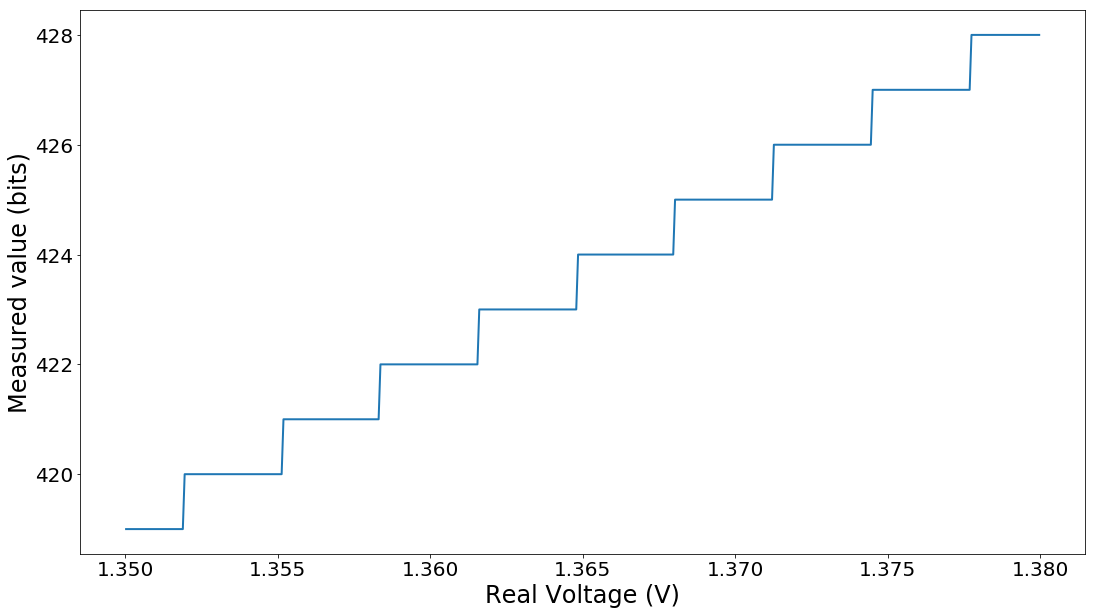
\includegraphics[width=.6\textwidth]{images/Chapter_03/digitalization.png}
\end{center}

The figure above shows a detail of how the digitalization looks like for a range of voltages. You see the discrete steps that the digital value takes for different voltages. Digitizing signals is a critical topic for anybody working in the lab. There is a whole set of ramifications regarding visualization, data storage, and more.

Particularly, the {PFTL DAQ} has a different behavior for reading than for setting values. The output channels take $4095$ ($2^{12}-1$) different values, i.e. they work with 12 bits instead of 10. Knowing the number of bits, also allows us to calculate the minimum difference between two output values:

\begin{equation}
 \frac{3.3\,\textrm{V} - 0\,\textrm{V}}{4096} \approx 0.0008\,\textrm{V} = 0.8\,\textrm{mV}
\end{equation}

The equation above shows how the resolution of the experiment is affected by the digitalization of the signals. We can't create voltages with a difference between them below $0.8\,\textrm{mV}$, and we are not able to detect changes below $3\,\textrm{mV}$. Later in the book, we come back to this discussion when we need to decide some parameters for visualizing our data.

Digitizing is everywhere. Digital cameras have a certain \emph{bit depth}, which tells us which range of values they can cover or, in other words, their dynamic range. Oscilloscopes, function generators, acquisition cards, they all have a precise digital resolution. When planning experiments, we always need to keep an eye on these values to understand if the devices are appropriate for the measurement we want to perform.

\exercise{We have used a for-loop to switch on and off the LED, and we have also displayed the voltage measured, but without units. Update the code so that instead of printing integers it prints the read value in volts.}

\section{Doing an experiment}
At this stage, we can easily communicate with the device; we can set an output and measure a voltage. It means that we have developed everything that we needed to measure the current that goes through the LED. We only need to combine setting an analog output and then reading an analog input. Since we are going to develop this with a more consistent approach, we leave it as an exercise:

\exercise{Write a method that allows you to linearly increase an analog output in a given range of values for a given step. \textbf{Hint:} the function \texttt{range} allows you to do this: \texttt{range(start, stop, step}. If you use this method, you should be able to see the LED switching gradually on.}

\exercise{Improve the method so that we can read analog values and store them once the measurement is complete. Returning the values can be a good idea so that we can use them outside of the object itself.}

\exercise{If you already have some experience with Python, you can also make a plot of the results. We cover this topic, later on, so don't stress too much about it now.}

If you tried to solve the exercises, you probably noticed that by having classes, our code is straightforward to use. It would be simple to share it with a colleague that has the same device, and they can adapt and expand it according to their needs. We should also keep in mind that when working with devices, it may very well be that someone else has already developed a Python driver for it, and we can just use it. One of the keys to developing sustainable code is to compartmentalize different aspects of it. Don't mix the logic of a particular experiment with the capabilities of a device, for example, is precisely the topic of the following chapter.

\textbf{Remember the Onion}: We have discussed in the Introduction, that we should always remember the onion principle when developing software. If we see the outcome of these last few exercises, we notice that we are failing to follow the principle. We have added much functionality to the driver class that does not reflect what the device itself can do. The {PFTL DAQ} doesn't have a way of linearly increasing an output, and we have achieved that new behavior with a loop in a program. Therefore, the proper way of adding extra functionality would be by adding another layer to the program, as we see in the next chapter.

Before moving forward, it is also important to discuss other libraries that may come in handy. We are not the first ones who try to develop a driver for a device. The pattern of writing and reading, initializing, and many more that we haven't covered, were faced by many developers before ourselves. It means that there are libraries already available that can speed up a lot the development of drivers. Let's see some of them.

\section{Using PyVISA}\label{section:pyvisa}
Some decades ago, prominent manufacturers of measurement instruments sat together and developed a standard called \href{https://en.wikipedia.org/wiki/Virtual_instrument_software_architecture}{Virtual instrument software architecture}, or VISA for short. This standard allows communicating with devices independently from the communication channel selected, and from the backend chosen. Different companies have developed different backends, such as NI-VISA, or TekVISA, but they \emph{should} be interchangeable. The backends are generally hard to install and do not work on every operating system. But they do allow to switch from a device connected via Serial to a device connected via USB or GPIB without changing the code.

To work with VISA instruments, we can use a library available for Python called \texttt{pyvisa}. There is also a pure Python implementation of the VISA backend called \mintinline{python}{pyvisa-py}, which is relatively stable even if it is still work in progress. It does not cover 100\% of the VISA standard, but for simple devices like the {PFTL DAQ} it should be more than enough. For complex projects, the solutions provided by vendors such as Tektronix or National Instruments may be more appropriate. In the next few paragraphs, we see how to get started with pyvisa-py, but it is not a requirement of the book. We decided to show it here to have it as a reference for other projects.

First, we need to install \mintinline{python}{pyvisa}, which is a wrapper around the VISA standard. Either with pip:

\begin{minted}{bash}
 pip install pyvisa
\end{minted}

Or with conda:

\begin{minted}{bash}
 conda install -c conda-forge pyvisa
\end{minted}

In case we don't have a VISA backend on our computer, we need to install one, and the easiest is the python implementation:

\begin{minted}{bash}
 pip install pyvisa-py
\end{minted}

or with conda:

\begin{minted}{bash}
 conda install -c conda-forge pyvisa-py
\end{minted}

There is also an interesting dependency missing: PySerial. Neither Pyvisa nor Pyvisa-py depend on PySerial. If we are going to communicate with serial devices, we should install that package ourselves (and the same is true for USB, GPIB, or any other communication standard.) The documentation of pyvisa-py\footnote{https://pyvisa-py.readthedocs.io} has handy information.

To quickly see how to work with PyVISA, we can start in a python interpreter, before going to more complex code. VISA allows you to list your devices:

\begin{minted}{pycon}
 >>> import visa
 >>> rm = visa.ResourceManager('@py')
 >>> rm.list_resources()
 ('ASRL/dev/ttyACM0::INSTR',)
 >>> dev = rm.open_resource('ASRL/dev/ttyACM0::INSTR')
 >>> dev.query('IDN')
 'PFTL DAQ Device built by Python for the Lab v.1.2020\n'
\end{minted}

We make explicit the backend we want to use by calling \texttt{ResourceManger}. In some cases, visa can automatically identify the backend on the computer. Then, we list all the devices connected to the computer. Bear in mind that this depends on the other packages that we installed. For example, we have only PySerial, and therefore pyvisa-py only lists serial devices. We can install PyUSB to work with USB devices, or GPIB, and so forth. The rest of the code is very similar to what we have done before. It becomes clear why we decided to call \emph{resource} the communication with the device.

Pay attention to the \texttt{query} method that we use to get the serial number from the device. We didn't develop it. PyVISA already took care of defining query for us. Not only PyVISA takes care of the query method, but they have plenty of options that we can use, such as transforming the output according to some rules or establishing the write termination. If we were to follow the pyVISA path, we could start by reading their documentation\footnote{https://pyvisa.readthedocs.io}.

\textbf{Why didn't we start with pyVISA?}. There are several reasons. One is pedagogical. It is better to start with as few dependencies as possible, so we can understand what is going on. We had to understand not only what commands are available, but we also had to be aware of the encoding and line termination. We made explicit the fact that to read from a device, we first have to write something to it. Once you gain confidence with the topics covered in this chapter, you can explore other solutions and alternatives. PyVISA is only the tip of the iceberg.

\section{Introducing Lantz}\label{section:lantz}
Defining a class for your device was a massive step in terms of usability. You can easily share your code with your colleagues, and they can immediately start using what you have developed with really few extra lines of code. However, there are many features that we may want but that someone needs to develop. For example, imagine that we want to limit the number of times the output voltage can change, or we don't want to write to the device always the same value, the first time was enough.

We may want to establish some limits, for example, to the analog output values. Imagine that we have a device that can handle up to $2.5\,\textrm{V}$. If we set the analog output to $3\,\textrm{V}$, we would burn it. Fortunately, there are some packages written especially to address this kind of problem. We are going to mention only one because it is a project with which we collaborate: \href{https://github.com/lantzproject/lantz}{Lantz}. You can install it by running:

\begin{minted}{bash}
pip install lantzdev
\end{minted}

\note{We introduce Lantz here for you to see that there is much room for improvement. However, through this book, we are not going to use it, and
that is why it was not a requirement when you were setting up the environment. Lantz is under development, and therefore some of the fine-tuned options may not work correctly on different platforms. Using Lantz also shifts a lot of the things you need to understand under-the-hood, and it is not what we want for an introductory course. If you are interested in learning more about Lantz and other packages, you should check for the Advanced Python for the Lab book when you finish with this one.}

Lantz is a Python package that focuses exclusively on instrumentation. We suggest you check their documentation and tutorials since they can be very inspiring. Here we just show you how to write your driver for the {PFTL DAQ} device using Lantz, and how to take advantage of some of its options. Lantz can do much more than what we show you here, but with these basics, you can start in the proper direction. You can also notice that some of the decisions we made earlier were directly inspired by how Lantz works.

Let's first re-write our driver class to make it Lantz-compatible, we start by importing what we need and define some of the constants of our device. We also add a simple method to get the identification of the device. Note that the first import is \texttt{MessageBasedDriver}, precisely what we have discussed at the beginning of the chapter.

\begin{minted}{python}
from time import sleep

from lantz import MessageBasedDriver, Feat


class MyDevice(MessageBasedDriver):

    DEFAULTS = {'ASRL': {'write_termination': '\n',
                        'read_termination': '\n',
                        'encoding': 'ascii',
                        }}

    @Feat()
    def idn(self):
        return self.query('IDN')


dev = MyDevice.via_serial('/dev/ttyACM0')
dev.initialize()
sleep(1)
print(dev.idn)
\end{minted}

There are several things to point out in this example. First, we have to note that we are importing a special module from Lantz, the \mintinline{python}{MessageBasedDriver}. Our class \mintinline{python}{MyDevice} inherits from the \mintinline{python}{MessageBasedDriver}. There is no \mintinline{python}{__init__} method in the snippet above. The reason for this is that the instantiation of the class is different, as we see later. The first thing we do in the class is to define the \mintinline{python}{DEFAULTS}. At first sight, they look the same as the ones we have defined for our driver. The \mintinline{python}{ASRL} option is for serial devices. In principle, we can specify different defaults for the same device, depending on the connection type. If we were using a {USB} connection, we would have used \texttt{USB}, or \texttt{GPIB} instead of, or in addition to \texttt{ASRL}.

The only method that we have included in the example is \mintinline{python}{idn} because, even if simple, it already shows some of the most interesting capabilities of Lantz. First, we can see that we have used \texttt{query} instead of \texttt{write} and \texttt{read}. Indeed, Lantz depends on pyVISA, so what is happening here is that under the hood, you are using the same command that we saw in the previous section. Bear in mind that Lantz automatically uses the write and read termination.

An extra syntactic thing to note is the \texttt{@Feat()} before the function. It is a \texttt{decorator}, one of the most useful ways of systematically altering the behavior of functions without rewriting. Without entering too much into details, a decorator is a function that takes as an argument another function. In Lantz, when using a \texttt{Feat}, it checks the arguments that you are passing to the method before actually executing it. Another advantage is that you can treat the method as an attribute. For example, you can do something like this \texttt{print(dev.idn)} instead of \texttt{print(dev.idn())} as we did in the previous section.

\exercise{Write another method for getting the value of an analog input. Remember that the function should take one argument: the channel.}

To read or write to the device, we need to define new methods. If you are stuck with the exercise, you can find inspiration from the example on how to write to an analog output below.

\begin{minted}{python}
output0 = None

[...]

@Feat(limits=(0,4095,1))
def set_output0(self):
    return self.output0

@set_output0.setter
def set_output0(self, value):
    command = "OUT:CH0:{}".format(value)
    self.write(command)
    self.output0 = value
\end{minted}

What we have done may end up being a bit confusing for people working with Lantz and with instrumentation for the first time. When we use \texttt{Features} in Lantz, we have to split the methods in two: first, a method for getting the value of a feature, and then a method for setting the value. We have to trick Lantz because our device doesn't have a way of knowing the value of an output. When we initialize the class, we create an attribute called \texttt{output0}, with a \texttt{None} value. Every time we update the value of the output on channel 0, we are going to store the latest value in this variable.

The first method reads the value, pretty much in the same way than with the \texttt{idn} method. The main difference here is that we are specifying some limits to the options, exactly as the manual specifies for the {PFTL DAQ} device. The method \texttt{set\_output0} returns the last value that has been set to the channel 0, or \texttt{None} if it has never been set to a value. The \texttt{@Feat} in Lantz, forces us to define the first method, also called a \texttt{getter}. It is the reason why we have to trick Lantz, and we couldn't simply define the \texttt{setter}. On the other hand, if the setter is not defined, it means that you have a read-only feature, such as with \texttt{idn}. The second method determines how to set the output and has no return value. The command is very similar to how the driver you developed earlier works. Once we instantiate the class, we can use the two commands like this:

\begin{minted}{python}
print(dev.set_output0)
dev.set_output0 = 500
print(dev.set_output0)
\end{minted}

Even if the programming of the driver is slightly more involved, we can see that the results are clear. A property of the real device also appears as a property of the Python object. Remember that when you execute \texttt{dev.set\_output0 = 500}, you are changing an output in your device. The line looks very innocent, but it isn't. Many things are happening under the hood both in Python and on your device. I encourage you to see what happens if you try to set a value outside of the limits of the device, i.e., try something like \texttt{dev.set\_output0 = 5000}.

The method we developed works only with the analog output 0. It means that if we want to change the value of another channel, wet have to write a new method. It is both unhandy and starts to violate the law of the copy/paste. If we have a device with 64 different outputs, it becomes incredibly complicated to achieve a simple task. Fortunately, Lantz allows us to program such a feature without too much effort:

\begin{minted}{python}
_output = [None, None]

[...]

@DictFeat(keys=[0, 1], limits=(0, 4095, 1))
def output(self, key):
    return self._output[key]

@output.setter
def output(self, key, value):
    self.write(f'OUT:CH{key}:{value}')
    self._output[key] = value
\end{minted}

Because the {PFTL DAQ} device has only two outputs, we initialize a variable \texttt{output} with only two elements. The main difference here is that we don't use a \texttt{Feat} but a \texttt{DicFeat}, which ill take two arguments instead of one: the channel number and the value. The \texttt{keys} are a list containing all the possible options for the channel. The values, such as before, are the limits of what We can send to the device. The last \texttt{1} is there just to make it explicit that we take values in steps of 1. We can use the code in this way:

\begin{minted}{python}
dev.output[0] = 500
dev.output[1] = 1000
print(dev.output[0])
print(dev.output[1])
\end{minted}

And now it makes much more sense, and it is cleaner than before. We can also check what happens if we set a value outside of what we have established as limits. The examples above only scratch the surface of what Lantz can do. Sadly, at the moment of writing, the documentation for the latest version of Lantz is missing. The best starting point is the repository with the code: https://github.com/lantzproject.

With the examples above, there is a small step to understand how to solve the following:

\exercise{Write a \texttt{@DictFeat} that reads a value of any given analog input channel.}

\section{Conclusions}\label{section:conclusions}
We have covered many details regarding the communication with devices. We have seen how to start writing and reading from a device at a low level, straight from Python packages such as \emph{PySerial}. We have also seen that it is handy to develop classes and not only plain functions or scripts. We have briefly covered pyVISA and Lantz, two Python packages that allow you to build drivers in a systematic, clear, and easy way. The rest of the book doesn't depend on them, but you must know of their existence.

It is impossible in a book to cover all the possible scenarios that you are going to observe over time in the lab. You may have devices that communicate in different ways. You may have devices that are not message-based. The important point, not only in this chapter but also throughout the book, is that once you build a general framework in your mind, it is going to be much easier to find answers online and to adapt others' code.

Remember, documentation is your best friend in the lab. You always have to start by checking the manual of the devices you are using. Sometimes some manufacturers already provide drivers for Python. Such is the case of National Instruments and Basler, but they are not the only ones. Checking the manuals is also crucial because you have to be careful with the limits of your devices. Not only to prevent damages to devices but also because if you employ an instrument outside of the range for which it was designed, you can start generating artifacts in your data. When in doubt, always check the documentation of the packages you are using. PySerial, PyVISA, PyUSB, Lantz, they are quite complex packages, and they have many options. In their documentation pages, you can find a lot of information and examples. Moreover, you can also check how to communicate with the developers because they are very often able to give you a hand with your problems.

\section{Addendum 1: Unicode Encoding}\label{section:unicode}
We have seen in the previous sections that when we want to send a message to the device, we need to transform a string to binary. This process is called encoding a string. Computers do not understand what a letter is, they just understand binary information, 1s and 0s. It means that if we want to display an \texttt{a}, or a \texttt{b}, we need to find a way of converting bytes into a character, or the other way around if we want to do something with that character.

A standard that appeared several years ago is called ASCII. ASCII contemplates transforming 128 different characters to binary. Characters also include punctuation marks such as \texttt{.}, \texttt{!}, or \texttt{:}, and numbers. 128 is not a random number, but it is $2^7$. For the English language, 128 characters are enough. But for languages such as Spanish, which have characters such as \texttt{ñ}, French with its different accents, and without even mentioning languages that use a non-Latin script, forced the appearance of new standards.

Having more than one \textit{standard} is incompatible with the definition of a standard. Imagine that we write a text in French, using a particular encoding, and then we share it with someone else. That other person does not know which encoding we used and decides to decode it using a Spanish standard. What will the output be? Very hard to know, and probably very hard to read by that person. It is without considering what would happen if someone writes in Thai and shares it with a Japanese, for example.

It still happens with some websites which handle special characters very poorly. Depending on how people configure databases, some characters which do not conform to the English script are just trimmed. This unbearable situation gave rise to a new encoding standard called, as the title of this section suggests: \textbf{Unicode}.

Unicode uses the same definition as ascii for the first 128 characters. It means that any ascii document looks the same if decoded with Unicode. The advantage is that Unicode defines the encoding for millions of extra characters, including all the modern scripts, but also ancient ones such as Egyptian hieroglyphs. Unicode allows people to exchange information without problems.

Thus, when we want to send a command to a device such as the {PFTL DAQ}, we need to determine how to encode it. Most devices work with ASCII values, but since they overlap with the Unicode standard, there is no conflict. Sometimes devices manufactured outside of the US may also use characters beyond the first 128, and thus choosing Unicode over ascii is always an advantage. In Python, if we want to choose how to encode a string, we can do the following:

\begin{minted}{python}
 var = 'This is a string'.encode('ascii')
 var1 = 'This is a string'.encode('utf-8')
 var2 = 'This is a string with a special character ñ'.encode('utf-8')
\end{minted}

Utf-8 is the way of calling the 8-bit Unicode standard. The example above is quite self-explanatory. You may want to check what happens if, on the last line, you change \texttt{utf-8} by \texttt{ascii}. You can also see what happens if you decode with \texttt{ascii} a string encoded as \texttt{utf-8}.

One of the changes between Python 2 and Python 3 that generated some headaches to unaware developers was the out-of-the-box support for Unicode. In Python 3, you are free to use any utf-8 character not only in strings but also as variable names, while in Python 2, this is not the case. For example, this is valid in Python 3:

\begin{minted}{python}
 var_ñ = 1
\end{minted}

If you are curious to see how Unicode works, the Wikipedia article is very descriptive. Plus, the Unicode consortium keeps adding new characters based on the input not only from industry leaders but also from individuals. You can see the latest emojis added and notice that some were proposed by local organizations that wanted to have a way of expressing their idiosyncrasies.

    \chapter{Model-View-Controller for Science}\label{ch:mvcs}

\section{Introduction}\label{sec:mvc-introduction}
Developing a computer program is much more than having a few scripts that you can run when you need them. The software should take care of a lot of your concerns, such as the limits of your devices, and it should be flexible enough that it enables you to change what measurements you're performing without spending months changing the code base. More importantly, a program should be extensible in the long run, not just by you but also by future colleagues and, potentially, by anyone who finds your application online.

Therefore, when you develop software, you'll want to keep in mind the following \textbf{programmer's mantras}:

\begin{itemize}
\item What you develop should be readable by both current and future colleagues
\item It should be easy to add solutions that have been developed by others
\item The program should allow you to exchange devices that achieve the same goal (e.g., oscilloscopes of different brands)
\item The code developed in one context has to be available in other contexts (i.e., in other experiments)
\end{itemize}

Let's take a look at each of these in turn. The first mantra isn't too challenging to understand in and of itself. The second mantra talks about solutions developed by others, meaning that often another developer may have already written a driver for a device, or perhaps a measurement script. Therefore, it should be easy to get code from other developers and use their software in your projects.

The third mantra discusses exchanging hardware, which is something that's often not valued until it happens. In most labs, there's always a legacy device that sooner or later breaks down, and you'll need to replace it. In another case, you might move to a different lab and need to continue your experiments with different hardware. There are patterns that you can follow to allow a simple exchange of devices. The last mantra speaks about context. Experiments can be very different, but the logic behind them is often quite similar. You measure the I-V curve of a diode, but this is, by no means, any different from doing a 1-D scan on a confocal microscope, or tuning the wavelength of a laser.

The mantras are not rules. They're just points on which you should reflect to try and recognize when you're departing from the path you wanted to follow when you started your project. In the following sections, you're going to explore a design pattern for software that has many benefits when developing scientific software for controlling experiments. It's called \textbf{The Model-View-Controller for Science.}

\section{Understanding the MVCs Design Pattern}\label{sec:mvc}
\begin{center}
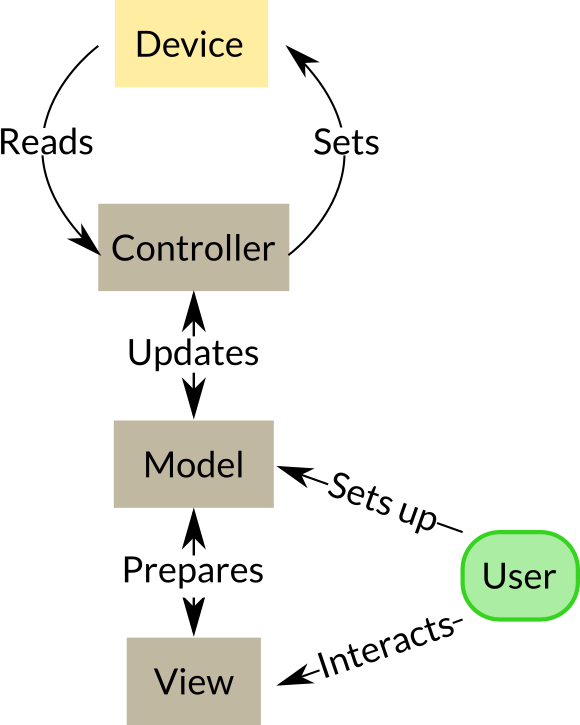
\includegraphics{images/Chapter_04/MVCs.png}
\end{center}

A \textbf{design pattern} is nothing more than a set of rules that determine where you can place different parts of the code and how they're going to interact with each other. One such pattern is called the \textbf{Model-View-Controller} pattern, or MVC for short. When you're working with devices in the lab, there's an extra layer that most computer programs lack, which is the interaction with the real world through specific devices. That's why we decided to nickname the pattern \textbf{MVCs}, with the "s" for \emph{science}. Let's take a closer look at each component of the MVC.

A \textbf{Controller} for the purposes of this book can also be called a \emph{driver}, which is responsible for communicating with devices. This can be a Python class you developed yourself, such as the one you built in the previous chapter, or it can be a Python package that was developed by someone else. For instance, many manufacturers provide drivers themselves, such as PyPylons from Basler, or the NI-DAQmx bindings for Python. The driver has to reflect the capabilities of the device, nothing more and nothing less. For example, if a device can acquire just one data point at a time, then the driver shouldn't include a function for acquiring an array of data using a loop. You saw this briefly in the previous chapter. Whatever belongs to the logic that a user imposes belongs to the Model component.

The \textbf{Model} is where all the logic is defined. This is where you determine how you're going to use a device for your experiment. A clear example would be the introduction of units. The \py{Device} class from the previous chapter takes only integer values as arguments of the methods. If you would like to transform that information into voltages, then you could do this in the model.

Moreover, in the experiment itself, you measure voltage, but you can convert it into a current with Ohm's law. This behavior is particular to your experiment, and thus the option shouldn't be hard coded in the driver. The place to include this information is the Model. The main advantage of splitting up \emph{Controllers} and \emph{Models} is that it becomes simple to upgrade or replace a device. You need to update the \emph{Model} to reflect the new options of the device, but the logic of the experiment is left intact.

There's a second type of model called the \textbf{Experiment Model} in which you link different devices to perform a measurement. You could also use a single device, but you add the features that an experiment needs (for example, saving data, plotting, analyzing, or transforming units). With straightforward cases, the boundary between the device model and the experiment model can be blurry. Still, when you're dealing with several devices or more complex workflows, it becomes much clearer. At the end of the book, we give a reference to some of the projects we've worked on, which can be a good source of inspiration.

The \emph{View} is the place where you can place everything related to how you show data to the user and how the user can change the parameters of the experiment. In practice, it's a collection of files that build up a Graphical User Interface ({GUI}). Within the {GUI}, you set, for example, the start, stop, and step of the experiment. This information is passed on to the model to acquire the data, save it, and plot it. Note, however, that the user interacts through the View with the Model, but never directly interacts with the Controller. It's also essential for you to keep in mind that all the logic is implemented in the Model. For example, if you save the data to files, the procedure to create new file names should be specified in the Model and not in the View.

For this project, the controller is what you learned about in Chapter~\ref{ch:first-driver}. The model for the device will be discussed in Chapter~\ref{ch:device-model}, the model for the experiment in Chapter~\ref{ch:experiment-model}, and the view in Chapters~\ref{ch:starting-gui} and~\ref{ch:user-input-designer}. As you can see, there are still many things to cover in the book. It's important to be patient, because you're going to grow a solution slowly, based on your needs, and solving the mistakes that may appear as you go, not just following a path blindly.

\tipsInfo{Why Separate the Code?}{For those who are new to developing code for the lab, it may be hard to understand why and how to split up the \emph{Controller} and the \emph{Model}. When you have only one device that you use for only one goal, one that is as simple as the device you're using in this book, the differences between Model and Controller are very thin. However, when you wish to include code developed by others, or when you want to share your own code, it's crucial that you separate the capabilities of your device from the logic of your experiment. If you don't do so, then all your code will only work when performing just one particular experiment.}

The meaning of \emph{Model}, \emph{View} and \emph{Controller} changes depending on each developer or community. People developing a web application are not dealing with devices in the real world, as those in the lab are. Therefore, the {MVC} pattern definition can change from one field to another. The details are not that important; once you establish a structure and follow it, then everyone else will be able to understand quickly what the code is doing and where. Once you understand what each component is, you will very quickly understand where you need to change the code to solve a bug or add new functionality.

\section{Structuring the Program}\label{sec:structure-of-theprogram}
In the program you're developing in this book, you follow the MVC design pattern quite literally. This means that you have to create three folders called \emph{Model}, \emph{View} and \emph{Controller}. In the previous chapter, you've already developed the driver for the device. Go ahead and move the file \textbf{pftl\_daq.py} into the \emph{Controller} folder.

\questionInfo{Exercise}{Create a file \textbf{analog\_daq.py} in the \emph{Model} folder. Inside the file, define a class called \mintinline{python}{AnalogDaq}. What methods do you think should belong to the device Model?}

In your definition of Model, it's vital for you to make a further distinction. On the one hand, you have models for the devices you use. In those models, you define things such as units or how to initialize the device. However, experiments often require you to perform complex tasks in which you need to synchronize several instruments. When you perform a measurement, you need to save the data or load the configuration from a file.

\questionInfo{Exercise}{Create a file in the \emph{Model} folder called \textbf{experiment.py}. Define a class called \mintinline{python}{Experiment} and add some methods that you think are going to be useful. You can, for example, add a method for switching on or off the {LED}. You can also add a method for doing a scan of an analog output signal.

The methods can be empty, so don't worry about making it work, but focus on the layout. You have to start thinking about the parameters that you need and the order in which you can call every method. For example, to save the data, you need to specify a folder first.}

The \emph{View} folder is going to require a bit more work than the other two. However, you can already start thinking about how the user is going to interact with your program. Most likely, you have thought that sometimes the {LED} will be plugged into output channel number 1, and other times to channel number 0. You don't want to change the code every time you change where you've connected the LED. The same happens, for instance, with the channel you want to monitor, or the time delay between steps. You'll include all this behavior in the View that you'll develop in the last chapters of the book.

Now that you've started to split the code into different folders and files, it's essential for you to learn how to make programs that can use the code that's located in those separate files. This process is called \textbf{importing}, and it's the focus of the next section.

\section{Importing Modules in Python}\label{sec:importing-python}
In the previous chapter, you saw some lines that look like this:

\begin{minted}{python}
import numpy as np
from time import sleep
\end{minted}

The first line imports the NumPy package, but changes its name to \mintinline{python}{np}. Changing the name makes it easier for you to work with libraries, since you can type fewer letters (\mintinline{python}{np} instead of \mintinline{python}{numpy}). The second line is importing one specific function from a package called \mintinline{python}{time}. It's important for you to realize that the import process is different in both cases. NumPy is a complex package, with many modules that you can use. The same is true for \emph{time}. However, in the lines above, you have only imported the module \emph{sleep} from the package \emph{time}. If you want to use it, you can do this:

\begin{minted}{python}
sleep(1)
\end{minted}

With \emph{Numpy}, you will need to specify which module you want:

\begin{minted}{python}
np.random.random(1)
\end{minted}

If you know you only want to use \mintinline{python}{random} from NumPy, then you can also import and use it like this:

\begin{minted}{python}
from numpy.random import random

random(1)
\end{minted}

You may wonder why you would import all of NumPy if you're just using one of its functions. Well, the name \emph{random} is not defined solely by NumPy. Python also provides its own \py{random} module. You can import it like this:

\begin{minted}{python}
import random
\end{minted}

If you needed both \emph{random} functions (the one from NumPy and the one from Python's standard library) in the same program, you would have a clash. How could you be sure that you're using NumPy's function and not Python's? What's more, you might even define your own random function, and you would like to be able to choose which one to use. More importantly, you want to avoid generating unexpected behavior because of redefining functions without realizing it.

When working with your code, you can import different modules in the same way. Open a terminal and navigate to the root folder of the project. This is the folder that contains the \emph{Model}, \emph{View}, and \emph{Controller} folders. Start the Python interpreter, and then type this:

\begin{minted}{pycon}
>>> from Controller.pftl_daq import Device
\end{minted}

Now you have the controller available for use. You can then do the following:

\begin{minted}{pycon}
>>> dev = Device('/dev/ttyACM0')
>>> dev.initialize()
\end{minted}

However, something strange happens if you run the code above. As soon as you import \py{Device}, the program starts communicating with the device, outputs the identification number, and switches on and off the LED. This behavior is something you don't want, and this is a very common pitfall for Python developers. Of course, you don't want the code to trigger a measurement just because you imported the module into your program.

To avoid having the code run as soon as an import happens, you must change the file \textbf{pftl\_daq.py}. You can add one line of code at the end of the file, as well as some indentation, to make it look like this:

\begin{minted}{python}
if __name__ == "__main__":
    dev = Device('/dev/ttyACM0') #<---- Remember to change the port
    dev.initialize()
    serial_number = dev.idn()
    print(f'The device serial number is: {serial_number}')
    for i in range(10):
        dev.set_analog_output(0, 4000)
        volts = dev.get_analog_input(0)
        print(f'Measured {volts}')
        sleep(.5)
        dev.set_analog_output(0, 0)
        volts = dev.get_analog_input(0)
        print(f'Measured {volts}')
        sleep(.5)
\end{minted}

To see the changes, you first must close Python by running the \py{exit()} command and then open it again. Python won't import the same modules twice, so it won't realize that the file with your Controller changed. After you restart Python, you can try to import the Controller again. Now, things are going to look fine, and you can use the \py{Device} as you intended. You can leave the space at the bottom of the files to hold examples of how to use the code above. If you ever find the Device around, and you don't remember what you were supposed to do with it, you can always go to the bottom of the file and see how it works.

Every time you encounter a behavior that's not easy to understand, the best idea is for you to transform it into simpler components and explore them one by one. In this case, the import process may be a bit confusing. To understand it a bit more, especially with respect to how the line \mintinline{python}{if __name__} works, you can create a new file called \textbf{dummy\_controller.py} in the \emph{Controller} folder with the following lines of code:

\begin{minted}{python}
print('This is the dummy Controller')

def dummy_example():
    print('This is a function in the dummy Controller')

if __name__ == '__main__':
    print('This is printed only from __main__')
    dummy_example()

\end{minted}

\sloppy From the Terminal, you can just type \py{python Controller.dummy_controller.py}. The output should be like what you see below:

\begin{minted}{bash}
This is the dummy Controller
This is printed only from __main__
This is a function in the dummy Controller
\end{minted}

What you see is that the entire code was executed.

\questionInfo{Exercise}{What do you expect to happen if you run \mintinline{python}{import dummy_controller}?}

Things are going to be different when you import the file. In the Python interpreter you can do the following:

\begin{minted}{pycon}
>>> from Controller import dummy_controller
This is the dummy Controller
>>> dummy_controller.dummy_example()
This is a function in the dummy Controller
>>> from Controller.dummy_controller import dummy_example
>>> dummy_example()
This is a function in the dummy Controller
\end{minted}

First, notice that the code at the end never gets executed. This means that the \py{if} statement is not \py{True}. This block is handy when you want to have code that works as a standalone (when you execute it directly, for example), but you don't want to execute those lines if you import. In the case of the real Controller, we wanted to leave some examples at the end to show how you can use it, but when you're importing a class, you don't want it to start communicating with the device.

\sloppy You can also see that the line \py{"This is the dummy Controller"} appears only once. Python knows that you've already imported the module \textbf{dummy\_controller}, and it won't execute those import lines again. Therefore, you have to be aware that it's not a matter of using the \py{from} in the importing procedure. You can close Python, start it again and revert the order in which you import, and the print will still be there the first time but not the second. It means that Python is smart when importing modules, and it won't fetch the elements it already has available, even if you're importing in a slightly different way.

\tipsInfo{Naming Conventions}{We should establish some naming conventions to avoid confusion later on. In Python, any file that defines variables, functions, or classes is called a \mintinline{python}{Module}. The folder that contains modules is called a \mintinline{python}{Package}.}

Python imports might be easier to work with than they are to understand, especially when you're trying to pay attention to all the different definitions. The Official Python Documentation\footnote{https://docs.python.org/3.6/tutorial/modules.html} has an excellent chapter covering a lot of the ideas discussed. Many of the properties and behaviors can be learned through trial and error, though this can be very time consuming, and it may lead to unexpected errors.

There's one final remark that's worth mentioning about packages. Right now, you have three folders in your project: \emph{Model}, \emph{View}, and \emph{Controller}. But what would happen if you added a new folder called, for example, \emph{serial}? Next time you try to \py{import serial}, how would Python know whether it's supposed to import the PySerial library or your package? This can also happen the other way around. Perhaps you don't know that there's something already called \emph{Controller} in Python, and you don't care about this module; you want to import your own modules.

For Python to understand that a folder is a \emph{package}, you should add an empty file to the folder called \textbf{\_\_init\_\_.py}. This file is the way of letting Python know that a folder is more than just a plain directory, and thus it should be treated accordingly. In other words, you must add the empty init files in the three folders you have created so far. If you're using a Python IDE, such as PyCharm, notice that these files are created automatically if you chose 'new package' while trying to add a folder.

\questionInfo{Exercise}{Create a folder called \emph{random} and inside of that create a new file called \textbf{test.py}. Define a function inside the file. It's not important what it does. Then, save it. Start Python and see what happens if you run \mintinline{python}{from random import test}. Quit the interpreter and add an empty file called \textbf{\_\_init.py\_\_} inside the \textbf{random} folder. Try to import \py{test} again and see what happens.}

The init files of packages allow you to specify more complex behaviors when importing, but that goes beyond the scope of this book. Going through other packages is an excellent way of understanding how developers have decided to structure their code.

\section{Changing the PATH Variable}\label{sec:path}
There is still a huge difference between your code and the way a library, such as \emph{Numpy}, can be imported. \emph{Numpy} can be imported regardless of where you have started the Python interpreter. You can go to any folder in the Terminal, start Python and import numpy. However, you can import your package only if you're in its directory. If you're sitting on a different folder and try to import the Controller, you get an error like the following:

\begin{minted}{pycon}
>>> from Controller.pftl_daq import Device
Traceback (most recent call last):
  File "<stdin>", line 1, in <module>
ModuleNotFoundError: No module named 'controller'
\end{minted}

Python searches for packages in specific locations, and once it finds one, it stops searching. \emph{Numpy} is located in one of the folders that Python uses, but Python is not aware of your package yet. One way to let Python know where your package is located, is by adding the folder to a system variable called \emph{PYTHONPATH}.

On Windows, you can follow the steps explained in Section~\ref{subsec:path-windows}, when you were dealing with the details of adding environment variables after installing Python. The only difference is that you should use the variable PYTHONPATH instead of just PATH. On Linux, it's enough to run the following command:

\begin{minted}{bash}
$ export PYTHONPATH=$PYTHONPATH":/path/to/PFTL"
\end{minted}

We have to change \py{/path/to/PFTL} with the full path to the folder where you're keeping the code. After doing that, you can type \py{from Controller import *} wherever you're in your computer, and Python finds the appropriate folder. On Linux, the change is not permanent, and you need to rerun the line next time you start the Terminal. You can modify environment variables permanently, but this goes too much into the details of the operating systems.

If you're using an IDE to develop and run the code, you may have noticed that there's no need to add anything to the Python path. It's one of the advantages of using robust programs to develop software. They take care of many things for us. However, at some point, it's also essential to be able to run the program independently of the editor software.

\section{Finalizing the Layout}\label{sec:final-layout}
At this stage, you should have a clear separation of the code into Model, Controller, and View. Most of them are, for the time being, empty folders. However, you're not limited to having only three folders in your project. Most likely, you want to provide some examples of how to use the code or some documentation.

However, if you create extra folders next to the three main ones, the structure of the program starts to be polluted. It won't be clear what is part of the program, and what is a user-specific setting. Therefore, it's a common practice to make a folder to hold all the program and, next to it, you create an extra folder to contain non-essential elements. In your case, the folder structure would look like this:

\begin{minted}{text}
├── Docs/
├── Examples/
└── PythonForTheLab/
    ├── Controller/
    │   ├── __init__.py
    │   └── pftl_daq_01.py
    ├── Model/
    │   └── __init__.py
    ├── View/
    │   └── __init__.py
    └── __init__.py
\end{minted}

There are three folders at the top level: \emph{Docs}, \emph{Examples} and \emph{PythonForTheLab}. The last one is holding the \emph{Model}, \emph{View} and \emph{Controller} with all the code that you have developed up to now. The \emph{PythonForTheLab} also requires an \textbf{\_\_init\_\_.py} file, because it's your main package. This folder structure would allow us to do the following:

\begin{minted}{pycon}
>>> from PythonForTheLab.Controller import pftl_daq
\end{minted}

This code is clearer than importing the Controller directly, because it also allows us to, in principle, have different programs at the same time and import only the elements you need from each one. For example, you could have one big project with many devices and complex measurements, and a smaller program to do more specialized tasks that only require \emph{some} of the devices.

\section{Conclusions}\label{sec:layout-conclusions}
Following a pattern when programming makes the code much easier to understand, to maintain, and to explain to others. Patterns, however, are not set in stone. Sometimes there's no clear divide between what you should develop where. The important thing is to be consistent. For example, if at some point it's decided that controllers should handle real-world units, then all controllers should do it. If, on the other hand, you agreed that models should handle units, then all models should do it, regardless of what the specific controllers do.

Following a pattern is useful not only when there are many developers involved in the same project, but also when the same person is working on different projects, or if they change labs, or experiments. As time passes, you start accumulating a collection of tools, and being able to transfer them from one experiment to another makes it much faster to have a measurement running without reinventing the wheel over and over again.

Another essential aspect for many scientists is that solutions should be developed as quickly as possible to test out new ideas. And this is how you laid out this book. First, you quickly manage to communicate with the device. You saw you can acquire data, switch on and off the LED. If the measurement would be a one-off task, then you would have finished. But if you would like to start changing parameters, or using the code for another experiment, then you must keep going. Expanding the code is what you're going to do next. In these sections, you have explored a sustainable way of following the \emph{Onion Principle}. Factoring also concerns about the speed at which you can implement a solution for the lab.

The strategies proposed in this chapter do not come naturally to every developer, and even if you know them, you can try to find shortcuts. The truth is that no one does an experiment only once. The key to better science is reproducibility, and the clearer the code that enabled you to acquire data, the easier it's to repeat a measurement, even by someone else. You can only lay out the foundations for what you consider a robust solution. If you find a different path, you're always free to follow it, but never miss the bigger picture from your sight.

    \chapter{Writing a Model for the Device}\label{chapter:device-model}

\section{Introduction}
The secret to successfully develop a model for a device is to think beforehand what do we expect from the device, how are we actually planning to use it. The first time we start thinking about models it can become complicated because we need to anticipate our future needs. For example, the {PFTL DAQ} device doesn't handle units. It would be great if the model would allow us to specify the output voltage instead of converting it to an integer because it is what the driver uses. This requirement seems trivial and probably is the first one that comes to mind. Later, once you really start using the program, you will see that some other useful options were missing, and you could have saved a lot of time if you would have thought about them. 

There is no magical recipe to teach exactly how to develop models for devices. Each device and each experiment will be special, the best we can do is to focus on the task at hand. The rest can be extrapolated to other devices and experiments. Once you understand the role that models play, you will be able to use them for very different purposes, without needing to re-write the entire program. With a simple device and a simple experiment the gain of having models separated from controllers may not be immediate, but as soon as the complexity grows, the value will become apparent. 

\warning{It is impossible to overestimate the importance of reading the manuals of your devices. Hardware in the lab is not the same as consumer hardware. Things can break, signals may not make sense. Be always sure to understand the limits under which each component operates.}

\section{Device Model}\label{devicemodel}
The first step when defining a model for a device is to think how do we want to interact with that piece of hardware. Of course, we would like to initialize the device, set a voltage, read a voltage and finalize the device. But we don't want to just repeat what the controller can do. When we initialize or finalize the device, we want to be sure the output voltages are set at $0\,\textrm{V}$. This ensures that no current will be flowing through the LED unless we explicitly want it. We also want to be able to use values in volts when setting an output, and getting values in volts when reading a voltage. 

We can develop a skeleton of the model, using empty methods, to have an idea of what we need to develop and the arguemtns and outputs of each method. Let's start by creating a file \textbf{analog\_daq.py} in the \emph{Model} folder, we can then add the following code:

\begin{minted}{python}
class AnalogDaq:
    def __init__(self, port):
        pass
    
    def initialize(self):
        pass
    
    def get_voltage(self, channel):
        pass
    
    def set_voltage(self, channel, volts):
        pass
    
    def finalize(self):
        pass
\end{minted}

New we can start step by setp. We start very similarly to how we started the controller, the \texttt{AnalogDaq} class takes port as argument for initializing. The main difference will be that we don't use PySerial directly, but we will use the controller, so we can start improving our code, like this:

\begin{minted}{python}
from PythonForTheLab.Controller.pftl_daq import Device
 
class AnalogDaq:
    def __init__(self, port):
        self.port = port
        self.driver = Device(self.port)
    
    def initialize(self):
        self.driver.initialize()
        self.set_voltage(0, 0)
        self.set_voltage(1, 0)
\end{minted}

We initialize the class by storing the \texttt{port} and by creating a \texttt{self.driver} attribute. Remember that the \texttt{Device} has a separate method for initializing. The \texttt{initialize} method now not only initializes the the driver itself, but also sets the output voltages to 0. We haven't developed a way of setting voltaes, yet, but we see the flow. The same works for the \texttt{finalize} method:

\begin{minted}{python}
    def finalize(self):
        self.set_voltage(0, 0)
        self.set_voltage(1, 0)
        self.driver.finalize()
\end{minted}

We first set the voltages to 0 and then we finalize the controller. This is a clear example of our own logic imposed to the device. In some cases, we don't want to set the voltage to 0 when closing the communication. Perhaps we are just switching on a laser and we want it to stay on even if we switch off the computer, or we are using piezo stages and is not recommended to suddenly shake them by setting a different voltage, it is better just to leave a voltage applied to them. That is why, adding these features to the controller would imply violating the separation of models and controllers. What we do with the voltages is part of the logic, not of the device itself. Now that we have this code, we can also add an example to the end of the file, to show how the model can be used:

\begin{minted}{python}
if __name__ == "__main__":
    daq = AnalogDaq('/dev/ttyACM0')
    daq.initialize()
    voltage = 3
    daq.set_voltage(0, voltage)
    input_volts = daq.get_voltage(0)
    print(input_volts)
    daq.finalize()
\end{minted}

The last missing bits are the methods for getting and setting a voltage. What we are going to do in these steps was discussed on Section \ref{subsection:digitazing}. To set a voltage, we first need to transform a voltage in the range $0-3.3$ to an integer in the range $0-4095$ and then we apply it:

\begin{minted}{python}
    def set_voltage(self, channel, volts):
        voltage_bits = voltage*4095/3.3
        self.driver.set_analog_output(channel, voltage_bits)
\end{minted}

And we can do the same for the get method:

\begin{minted}{python}
    def get_voltage(self, channel):
        voltage_bits = self.driver.get_analog_input(channel)
        voltage = voltage_bits*3.3/1023
        return voltage
\end{minted}

And that is all what is needed. We can now run the code and see that we are actually reading voltages and setting voltages. Because of how the experiment works, the values we get at the analog input are going to be very small, in the order of few tens of millivolts, but enough to be detected by the {PFTL DAQ}. 

\section{Base Model}\label{section:base-model}
In this book we are working with only one device, and therefore we are using only one model. But if we want to make our program compatible with more devices, we will need to start developing models for each new device. Since we have one model, it would look reasonable to copy it and adapt the methods based on what the new drivers allow us to do. Another option is to create a base class which will be inherited by all the models. In this way, we know that all the methods are defined, perhaps they don't do anything, but at least they are there. 

What we will do in this section is not a requirement to keep going, but is important to show the pattern, because sooner or later when the program grows, it will be a very useful approach. Create a file called \textbf{base\_daq.py} inside the Controller folder, we can add the following code to it:

\begin{minted}{python}
class DAQBase:
    def __init__(self, port):
        self.port = port
    
    def initialize(self):
        pass 
            
    def get_analog_value(self, channel):
        pass
    
    def set_analog_value(self, channel, value):
        pass
    
    def finalize(self):
        pass
\end{minted}

This class doesn't do anything by itself, it is only the schematics of what a model should contain. The \texttt{pass} that was added after every definition takes care of functions in which nothing happens. We can see that we specify also the arguments that each method will take, the initialize takes a port, setting a value takes channel and value and so forth. In programming, this is also called an API, or Application Programming Interface. The base class defines the interface that all the DAQ models will use. There will be an initialize method, a get and set analog and a finalize. Just by looking at this very simple example, we already know how things are going to work and what do we need to do to make them work. 

As an example, let's create a dummy DAQ that is able to generate random values when requested, and since it is not going to be connected to any real device, it will not do anything else. We can add the following code to \textbf{dummy\_daq.py} in the Models folder:

\begin{minted}{python}
from random import random
from PythonForTheLab.Model.daq_base import DAQBase

class DummyDaq(DAQBase):
     def get_analog_value(self, channel):
         return random()
\end{minted}

And if we copy the example code from our real daq, things are still going to work fine:

\begin{minted}{python}
if __name__ == "__main__":
    daq = AnalogDaq('/dev/ttyACM0')
    daq.initialize()
    voltage = 3
    daq.set_voltage(0, voltage)
    input_volts = daq.get_voltage(0)
    print(input_volts)
    daq.finalize()
\end{minted}

Of course, when we set a voltage, initialize, or finalize the model nothing actually happens, but when we ask for a value, we get one. You see that the way of using this class is the same as the real model, and it took us only 3 lines of code to develop. Perhaps in the future you move to a more complex DAQ, such as an oscilloscope. If you maintain the same names for the methods of the model, everything will keep working in the same way. 

\exercise{Update the real model to inherit from the base class}

\section{Adding real units to the code}\label{section:pint}
The model for the {PFTL DAQ} device is working great, but it has one problem. It allows us to set the output in volts and reads a value in volts. But if we ever make the mistake of supplying the value in millivolts, the program won't work as expected. In real cases, it is very hard to remember the units that every method should take. Sometimes you have very different outputs and inputs with each one taking different units. Imagine you want to make a periodic signal, perhaps the device asks for the frequency, perhaps for the period. 

In Python we can overcome the limitations of working with plain numbers by using a package called \emph{Pint}, that allows us to work with \emph{real} units. Let's quickly see how Pint can be used with a simple example:

\begin{minted}{pycon}
>>> import pint
>>> ur = pint.UnitRegistry()
>>> meter = ur('meter')
>>> b = 5*meter
>>> type(b)
<class 'pint.quantity.build_quantity_class.<locals>.Quantity'>
>>> print(b)
5 meter
>>> c = b.to('inch')
>>> print(c)
196.8503937007874 inch
\end{minted}

First, we import the package and start the \emph{Unit Registry}. In principle, Pint allows us to work with custom-made units, but the fundamental ones are already included in their own \emph{Unit Registry}. Then, because of convenience, we define the variable \texttt{meter}, as actually the unit meter. Finally, we assign the value of \texttt{5 meters} to \texttt{b}. In this case, \texttt{b} is of type \texttt{Quantity}, therefore it is not just a number, but a number and a unit attached to it. \emph{Pint} allows us to convert between units, and this is how we create the variable \texttt{c}, which is 5 meters converted to inches. And things can get very interesting:

\begin{minted}{pycon}
 >>> b == c
 True
\end{minted}

Even if the numeric value of \texttt{b} and \texttt{c} is different, they are still equal to each other, exactly as we would have imagined. We can also work with more complex units:

\begin{minted}{pycon}
>>> d = c*b
>>> print(d.to('m**2'))
25.0 meter ** 2
>>> print(d.to('in**2'))
38750.07750015501 inch ** 2
>>> t = 2.5*ur('s')
>>> v = c/t
>>> print(v.to('in/s'))
78.74015748031496 inch / second
\end{minted}

So far we have always been transforming between units of the same type, i.e. a length in meters to a length in inches, etc. But Pint can also handle combined units such as what happens with voltage, current and resistance:

\begin{minted}{pycon}
>>> current = 5*ur('A')
>>> res = 10*ur('ohm')
>>> voltage = current*res
>>> print(voltage)
50 ampere * ohm
>>> print(voltage.to('V'))
50.0 volt
>>> print(voltage.m_as('mV'))
50000.0
\end{minted}

The snippet above shows you that Pint is able to understand the relationship between Amperes, Ohms, and Volts. There is one more feature that is important to point out: Pint is able to parse strings in order to separate the units from the numbers. For example, we can do the following:

\begin{minted}{pycon}
 >>> current = ur('5 A')
 >>> resistance = ur('10 ohm')
\end{minted}

Being able to parse strings so easily is going to make our life much easier when we will be dealing with user input. Now we have seen how to handle \emph{real} units on our code. However, the device still requires us to set the output using plain numbers. In the context of Pint, just the number, without the units is called the \emph{magnitude}. To get the magnitude out of a quantity, we can do the following:

\begin{minted}{pycon}
 >>> current = ur('5 A')
 >>> current_mag = current.m
 >>> print(current)
 5 ampere
 >>> print(current_mag)
 5
 >>> current_ma = current.m_as('mA')
 >>> print(current_ma)
 5000.0
\end{minted}

We start with a quantity called \texttt{current} of $5\,\textrm{A}$. If we just append the \texttt{.m} to the variable, we get the magnitude in whatever unit it is already expressed. If we want to be sure to get the magnitude in a specific unit, we use the command \texttt{.m\_as()}. In our case, we will need to transform the user input to an integer, and we will not need to assume it is in volts, we can transform it to volts before converting it to an integer. The \texttt{set\_analog\_value} method would look like this:

\begin{minted}{python}
def set_analog_value(self, channel, value):
    value_volts = value.m_as('V')
    value_int = round(value_volts/3.3*4095)
    self.driver.set_analog_value(channel, value_int)
\end{minted}

We transform the value to volts and get only the magnitude. Then we transform that value to bits, using the round function to get a true integer after the operation. We use that rounded value to set the output on the device. Our program is now very flexible since the user can provide the output value in whatever units she pleases, provided that they can be transformed to volts.

\exercise{Update the method \texttt{get\_analog\_value} so it generates an in volts. Pay attention to the fact that you will need to import pint and create the unit registry before you define your class in order to be able to use it.}

We should also update the method for getting a voltage in order to return a voltage and not a plain number. The code below only shows the parts that have changed or added, not the entire class:

\begin{minted}{python}
import pint

ur = pint.UnitRegistry()

[...]

    def get_voltage(self, channel):
        voltage_bits = self.driver.get_analog_input(channel)
        voltage = voltage_bits * ur('3.3V')/1023
        return voltage
\end{minted}

However, we also need to update the \texttt{initialize} and \texttt{finalize} methods in order to use units and not plain numbers:

\begin{minted}{python}
def initialize(self):
    self.driver = Device(self.port)
    self.set_voltage(0, ur('0V'))
    self.set_voltage(1, ur('0V'))
            
def finalize(self):
    self.set_voltage(0, ur('0V'))
    self.set_voltage(1, ur('0V'))
    self.driver.close()
\end{minted}

The class is complete and we need to update the example code at the bottom of the file in order to use the real units:

\begin{minted}{python}
if __name__ == "__main__":
    daq = AnalogDaq('/dev/ttyACM0')
    daq.initialize()
    voltage = ur('3000mV')
    daq.set_voltage(0, voltage)
    input_volts = daq.get_voltage(0)
    print(input_volts)
    daq.finalize()
\end{minted}

If you are hesitant about the impact that different unit systems can have, there is a great example involving a multi-million dollar satellite. You can check the \href{http://articles.latimes.com/1999/oct/01/news/mn-17288}{news article}\footnote{http://articles.latimes.com/1999/oct/01/news/mn-17288} with the story of how the Mars Climate Orbiter fell from its orbit because engineers from the US failed at using the established units of measure in their software, resulting in a mix of metric and imperial systems. 

\section{Testing the DAQ Model}
At this point, we have a very functional program. We are able to handle units, we have split the logic of the units from the driver, meaning that we can easily share our code with colleagues or the rest of the world. It is time to test our program. On of the reasons we created the Examples folder was to be able to add extra python files that don't belong to our core program. In the Examples folder, create a file called \textbf{test\_daq.py}, and we can start using the model to do some measurements:

\begin{minted}{python}
import numpy as np
import pint

from PythonForTheLab.Model.analog_daq import AnalogDaq

ur = pint.UnitRegistry()
V = ur('V')

daq = AnalogDaq('/dev/ttyACM0') # <-- Remember to change the port

# 11 Values with units in a numpy array... 0, 0.3, 0.6, etc.
volt_range = np.linspace(0, 3, 11) * V 
current = [] # Empty list to store the values

for volt in volt_range:
    daq.set_analog_value(0, volt)
    current.append(daq.get_analog_value(0))

print(current)
\end{minted}

We can run the code above, but we will get the following error:

\begin{minted}{python}
 [...]
 ValueError: Cannot operate with Quantity and Quantity of different registries.
\end{minted}

The error is descriptive, but hard to understand if you are not aware of how Pint works. The unit registry is a collection of rules that allows us to transform from one quantity to another. But this rules belong to a unit registry. In principle, two distinct unit registries hold rules for different sets of units. This means that we can't convert units across unit registries. We need to use only one registry throughout the program. Right now, we are creating the registry in two different places: The device model and the example. 

Since units belong to the entire program, it could be a good idea to define the unit registry at the root. This means, creating it directly in the \textbf{\_\_init\_\_.py} file that we placed in the PythonForTheLab folder:

\begin{minted}{python}
 import pint
 
 ur = pint.UnitRegistry()
\end{minted}

Every time we want to use units and the unit registry, we will be able to do the following:

\begin{minted}{python}
 from PythonForTheLab import ur
\end{minted}

\exercise{Improve DAQ model in order to use the main unit registry and not one defined locally.}

\exercise{Modify the example that we developed for testing the DAQ model so it uses the main unit registry, and see that it works as expected.}

After completing the exercises above, we should be able to run the example and get the values we wanted. Something that should grab your attention is that we are storing volts in a variable called \texttt{current} which is highly anti-intuitive. We can transform the voltage measured to a current provided that we know which resistance are we using. In most cases, the resistance has a value of $100\,\textrm{Ohm}$, so we can do the following:

\begin{minted}{python}
 resistance = ur('100ohm')
 voltage = daq.get_analog_value(0)
 current = voltage/resistance
\end{minted}

\section{Appending to the PATH at runtime}\label{section:appending-path}
In Section \ref{section:path} we have seen how to add the root folder of the project to the computer's PYTHONPATH. This allows Python to find our program and allows us to import the packages and modules very easily. However, altering environment variables in different Operating Systems is not only cumbersome, it can also lead to unwanted results. For example, we may be over writing someting important if there is any name clash between the program we develop and some other library on the computer. 

Therefore, we can go a different route, and add the the folder to the path directly from within Python. This change will not be permanent, it will be in place only while the program runs, but no further. First, we need to learn how to identify the folder we want to add to the path. For this, Python offers a module called \texttt{os}. The code below looks cumbersome, but we will explain it after. This can be added at the begginig of the \textbf{test\_daq.py} file:

\begin{minted}{python}
import os

base_dir = os.path.dirname(os.path.dirname(os.path.abspath(__file__)))
\end{minted} 

First, \texttt{\_\_file\_\_} variable is a way of letting Python know we are interested in the current file, which in this case is \texttt{test\_daq.py}. If we go from inside to outside, we first get the absolute path to the file, this includes all the folders to get there. Then, we grab the directory that holds the file, which would be the \emph{Examples} folder. And then we grab the directory that contains the examples, which in our case is the root folder, or \texttt{base\_dir} as we called it. 

Next, we need to add the \texttt{base\_dir} to the path, for this we will use another package called \texttt{sys}, which is a wrapping for the operating system. This means that this package will adapt according to which operating system we use to run the program. To add the folder, we only need to do the following:

\begin{minted}{python}
import sys

sys.path.append(base_dir)
\end{minted}

And that is it. Doesn't matter if we modify the PYTHONPATH variable anymore, we can always run the \texttt{test\_daq.py} file. 

\warning{Since appending to path only works while the program runs, if we try to run the different files independently, Python will not know where to find the modules. The test files we create in Examples are what are called entry points, and the program should be run directly from them}

\section{Real World Example}\label{section:real-world-model}
The usefulness of models at this stage may still be obscure. We may be tempted to define units and transformation in the controller itself. We know we are the only ones using it, just to do one experiment. This may be fine when you start, but at some point, hopefully, the code will keep growing because the experiment will keep progressing. At Python for the Lab, we have developed software for controlling a microscope using a camera. However, in the lab there were several different cameras available, some more expensive and powerful, but that were shared between people. 

Therefore, having a flexible way of using different cameras for the same experiment became mandatory. Sometimes we would use a Hamamatsu, sometimes a Basler, sometimes a Photonics Science. However, each camera had an incredibily different way of working. First, Hamamatsu didn't provide any drivers written in Python. Photonics Science shared an internal tool they used, and Basler as an entire package called PyPylon to control their cameras. The controller layer therefore was not developed by us, but was given. 

At the model level, however, we made it sure that all cameras would work in the same way. They all have the same method for setting the exposure, or changing the region of interest. Therefore, the only thing that we needed to change to perform an experiment with one or the other camera was changing what model we were importing. The rest of the code would stay the same. If you want to see the real code, you can head to the repository on \href{https://github.com/uetke/UUTrack/tree/master/UUTrack/Model/Cameras}{Github}\footnote{https://github.com/uetke/UUTrack}. 

\section{Conclusions}\label{conclusions}
In this chapter we have seen what does \emph{Model} mean in the {MVC} pattern. We focus onto adding features to how the device works, such as switching off the outputs when we finalize using the device. We have also included real world units by using \textbf{Pint}, and learned some of its quircks regarding the unit registry. 

We have also covered how to append folders to the path through Python. This allows us to run all the import statements that we want, without having to manually alter the environment variables of the Operating System. This is very handy because on the one hand it runs unaltered in Linux, Windows, and Mac, on the other becasue we don't do any permanent changes to the configuration of the computer. It is a possibility that at some point we have two projects with the same name, because we use them for two different but very similar experiments, for example, but we want to be sure we are importing the correct one. 
    \chapter{Writing The Experiment Model}\label{chapter:experiment-model}

\section{Introduction}
In the \textbf{MVCs} design pattern, the \emph{Model} is where we should place the the logic and the decisions we make in order to perform a measurement. In the previous chapter we started specifying the logic of how we are going to use the DAQ device. We decided, for example, that the device should start and finish with the outputs set to $0\,\textrm{V}$, and that it should handle Pint units for setting and reading values. Even though it was a great start, there are still steps missing to perform a real experiment.

We are still missing, for example, the possibility to perform a scan in a given range of voltages, there is no way of saving data nor the parameters used to generate it. We can develop these tools in a script, and that is fine to get started. At some point, however, we want to be systematic, and we don't want to keep editing a script every time we must perform a measurement. We want the data to be consistently saved, or we want to enable other people to run their own experiments based on our routines.

This is when the \emph{onion principle} starts making sense. We are slowly building in complexity, one layer at a time. We started with the driver, built some logic on top of it through a device model, and now we can keep growing the complexity by defining an Experiment model. There are many different steps needed in order to perform a reproducible measurement, and we will cover them one by one. One important aspect we missing, on top of the ones mentioned earlier is, for example, transforming the voltages we measure to a current, so we can give sense to the \textbf{I} on the I-V curve we are trying to measure.

\note{With a simple device and experiment such as the one we use in this book, sometimes is hard to put a limit on what should go in the device model and what into the experiment model. There are no strict rules, we should always reflect on what we believe will be useful on the long run. Once we are confortable working with classes in Python, splitting the code into reusable, smaller modules does not lead to much more typing.}

There are two extra advantages of developing an experiment model which will become apparent only after working on these topics long engouh. On the one hand, the models are going to lead to reproducible experiments. If we keep track of the parameters we, we can go back exactly to the same conditions in which we have performed a specific measurement. On the other hand, once we are sure we can perform a measurement from the command line, running a script or within the Python interpreter, it is going to be very easy to build a Graphical User Interface ({GUI}) on top of it, but let's not get ahead of ourselves.

\section{The Skeleton of an Experiment Model}\label{section:skeleton-experiment-model}
Every time we want to start developing a model, it is handy to start from an empty skeleton. This will help us know what parts of the code need to be developed, what things we don't know how to do yet and need to learn. It also allows us to have a quick glimpse at how we expect our program to be used. We did it for the device model in the previous chapter, and we can do the same for the experiment in this chapter. First, we create a file called \textbf{experiment.py} inside the \emph{Model} folder, and then we think about the steps needed to perform a measurement:

\begin{minted}{python}
class Experiment:
    def __init__(self, config_file):
        pass

    def load_config(self):
        pass

    def load_daq(self):
        pass

    def do_scan(self):
        pass

    def save_data(self):
        pass

    def finalize(self):
        pass

\end{minted}

Most of the code should be self-explanatory, but some steps are worth mentioning. First, we include a \texttt{load\_config} method, which will rely on the \texttt{config\_file} we specify at the \texttt{\_\_init\_\_}. Having a separated config file will be useful not only to change parameters between measurements, but it will help us with our code. Especially when the number of things we need to remember grows, it is always handy to have a file where to look at how we named things.

We have also included a \texttt{load\_daq} method. So far, we have only one DAQ to use, but we go a bit ahead of time and assume that at some point there may be more than one and therefore we should have a way of loading one or the other. It can also be a case of premature optimization, in which we anticipate a future that never comes. Nevertheless, it is pedagogically useful to define it there.

The rest of the methods may seem intuitive enough. If we are missing extra pieces, we can always come back and add them. Now it is time to start developing each one of the building blocks.

\section{The Configuration File}\label{section:configuration-file}
\subsection{Working with YAML files}\label{subsection:yaml-files}
Before we keep developing code, we need to stop for a second to think what do we want our program to do. We need to think about what inputs are needed for our program. For example, we know we need the port in which the device is connected. We also know that we need to define an output and input channel, a range for the scan, a delay between data points, etc. Before going into the details, let's see how to easily store all these parameters into a text file.

In the \emph{Examples} folder, create a file called \textbf{experiment.yml}. This file can be created with any text editor, the only difference is the extension \emph{yml}. This file will hold all the parameters of the experiment. We are going to use a format called {YAML}, which has a straightforward structure, it looks like this:

\begin{minted}{yaml}
Experiment:
  name: This is a test Experiment
  range: [1, 10, 0.1]
  list:
   - first Element
   - second Element
\end{minted}

{YAML} is very simple to read both by a person and by the computer. It has just a few rules, the most important one is that the indentation is done with \textbf{2} spaces. In the example above, there is a main element called \textbf{Experiment}, everything that is indented compared to that element will belong to it. To read the file we are going to use a package called PyYAML, which was installed in Chapter \ref{ch:setting-up}. We can create a file called \textbf{test\_yaml.py} also in the Examples folder to understand how to use these files:

\begin{minted}{python}
import yaml

with open('experiment.yml', 'r') as f:
    e = yaml.load(f, Loader=yaml.FullLoader)

print(e['Experiment'])
for k in e['Experiment']:
    print(k)
    print(e['Experiment'][k])
    print(10*'-')
\end{minted}

We begin by opening the file using \mintinline{python}{open}. We use the \mintinline{python}{with} command because it is very handy for working with files and other resources that have the same pattern of opening/doing/closing. Yaml is then responsible for interpreting the information contained in the file. We store this information in a variable \texttt{e}, which turns out to be a dictionary.

The elements of dictionaries are addressed by keys. In the example above, there is a main key called \texttt{'Experiment'}, and the sub-keys \texttt{'name'}, \texttt{'range'} and \texttt{'list'}. If we want to use one of those elements, we can type \texttt{e['Experiment']['name']}, for example. The code prints out each element, separated by a horizontal line. Yaml imported the file directly as a dictionary but some of the elements are special. We can see that \texttt{'name'} is a string, but \texttt{'range'} and \texttt{'list'} are not. This will become very handy later on because YAML automatically detects what kind of information we are using.

\exercise{What type of variables has yaml generated for \texttt{'range'} and the \texttt{'list'}? (Remember that you can use \texttt{type(var)} to know the type of the variable.}

\exercise{YAML also supports numeric information. Create a new element and assign it a value of \texttt{1} or \texttt{3.14}. What kind of variable has YAML created in such cases?}

Of course, YAML can be used not only to read properties but also to save information generated in a program. Instead of loading data, we can use \texttt{yaml.dump} method to save it. For example, we can define a dictionary with the following information

\begin{minted}{python}
d = {'Experiment': {
    'name': 'Name of experiment',
    'range': [1, 10],
    'list': (1, 2, 3),}
}
\end{minted}

If we want to save it to a file, we can do the following:

\begin{minted}{python}
with open('data.yml', 'w') as f:
    f.write(yaml.dump(d, default_flow_style=False))
\end{minted}

We are using the \texttt{'w'} option to open the file, which means that every time we run the code, we will overwrite the file and lose the previous contents. After running the code we can open the file \textbf{data.yml} with any text editor and see that the contents are very similar to the one we created ourselves earlier. One of the advantages of the YAML format is that files are very easy to read, and don't require much typing.

\exercise{Read back the contents of \textbf{data.yml} and check that they are the same you saved.}

\exercise{Modify some of the values of \textbf{data.yml} directly with your text editor and see that those changes are reflected when you read again the file.}

\exercise{Create a numpy array and store it using yaml. How does it look like in the file? What happens if you read it back?}

\exercise{\textbf{Advanced}. Save a numpy array using yaml. Then activate a virtual environment in which PyYAML is available but not numpy. Try to load the contents of the file. What happens?}

Now that we know how to work with YAML files, it is time to start thinking about the experiment again. We need to stop and think about what do we need to know in order to perform an experiment.

\exercise{Create a new experiment.yml file in the \emph{Examples} folder. Use what you have learned about YAML files to write a file that contains all the information that you need to perform an experiment and interpret its data. For example, knowing \emph{who} performed an experiment may be important.}

\subsection{Loading the Config file}\label{subsection:loading-the-config}
We have decided to use YAML files because of their simplicity, and because it is easy to map them to dictionaries in Python. The main advantage of having a separated config file is not only that it will allow us to run different measurements changing the parameters, but that it will also help us keep our code organized. This will become much clearer later in this chapter.

First, we need to decide what are we going to include in the configuration file. The information is not static, it may very well happen that later we realize there is something important missing, and we added it, or something we thought was important is not necessary anymore. The idea is that every time we find ourselves making a decision about a value, that information should go to the config file. For example, if we need to decide in which port the DAQ is connected, that goes to the config file. We are going to use the \textbf{experiment.yml} file in the \emph{Examples} folder to store all this information. Below, we show how the config file could look like. We have included extra options that we haven't discussed yet, such as the user performing the experiment, which can be relevant for bookeeping:

\begin{minted}{text}
User:
  name: Aquiles

DAQ:
  name: AnalogDaq
  port: /dev/ttyACM0

Scan:
  start: 0V
  stop: 3.2V
  step: 400mV
  channel_out: 0
  channel_in: 0
  delay: 100ms

Saving:
  filename: data.dat # Files won't be overwritten, but renamed as data_001.dat, etc.
\end{minted}

We haven't used a main key such as \emph{experiment} because it does not add anything, and forces us to type more. If for some reason we needed to store parameters for two different experiments on the same file, then we could add two top-level keys such as \texttt{Experiment\_1}, \texttt{Experiment\_2}. The parameters above are enough to get started, and then slowly keep adding or modifying when we need. There are some obvious omissions, meant to trigger dicsussions further down the road. If you have already spotted them, you have done a good job, but don't stress yourself if you haven't.

We have to update the \texttt{Experiment} class to load the file. We are storing the filename within the class, so all our methods can be triggered without arguments. But this is just a choice we've made:

\begin{minted}{python}
import yaml

class Experiment:
    def __init__(self, config_file):
        self.config_file = config_file

    def load_config(self):
        with open(self.config_file, 'r') as f:
            data = yaml.load(f)
        self.config = data
\end{minted}

We have used the same code we showed in the previous section but as part of a method. When we load the configuration file, it will be stored as an attribute of the Experiment class, called \texttt{self.config}. Now that the experiment is starting to have shape, we can create a file to show how to use it and check whether we are doing things properly. In the \emph{Examples} folder, we can create a file called \textbf{run\_experiment.py}, and add the following:

\begin{minted}{python}
import sys
import os

base_dir = os.path.dirname(os.path.dirname(os.path.abspath(__file__)))
sys.path.append(base_dir)

from PythonForTheLab.model.experiment import Experiment

experiment = Experiment('experiment.yml')
experiment.load_config()
print(experiment.config)
\end{minted}

We use the strategy explained in Section \ref{section:appending-path} in order to let Python know where to find our program. The rest is easy to understand, we start an experiment, load the config file and print the parameters that we have loaded. So far, we are not doing much, but it is a good start.

Now we have a consistent interface for loading the configuration file into our programs. This gives us a great deal of flexibility and makes the code nicely reusable and extendable.

\exercise{When the function \texttt{load\_config} loads the configuration from a file, verify that some important parameters are defined. For example, verify that there is a user associated with an experiment. If there is something missing, print an error message or raise an Exception.}

\section{Loading the DAQ}\label{section:loading-daq}
To load the DAQ into our experiment, we can start with the simplest approach. We import the model for the daq, and we initialize it using the \texttt{load\_daq} method. We can update the experiment model, some parts of the code are omitted for brevity:

\begin{minted}{python}
from PythonForTheLab.Model.analog_daq import AnalogDaq

[...]

def load_daq(self):
    self.daq = AnalogDaq(self.config['DAQ']['port'])
    self.daq.initialize()
\end{minted}

The \texttt{load\_daq} method uses the information stored in the configuration file in order to instantiate and initialize the daq model. Having a config file in YAML format makes it very easy to navigate and find where the information of the port for the daq was located. The main key is \texttt{DAQ}, and the sub-key is \texttt{port}. In this way, there are much fewer things we need to keep in our heads, we can always go back to the file and read what we need to know. We have also decided that we initialize the device right after loading it. This could have been a separated method, but at this stage and for this experiment, there is no real need.

Since we are taking care of loading and initializing the DAQ, we can also develop the finalize method, which takes just one line:

\begin{minted}{python}
def finalize(self):
    self.daq.finalize()
\end{minted}

We can update the \textbf{run\_experiment.py} file to reflect the additions we have just made to the Experiment:

\begin{minted}{python}
[...]
experiment.load_daq()
print(experiment.daq)
experiment.finalize()
\end{minted}

When we run the code above, we will see that the output of of \texttt{print(experiment.daq)} is not pretty and it is hard to understand. We can update the device model in order to make the string that appears on screen nicer. We edit the \textbf{analog\_daq.py} file to include the following method in the \texttt{AnalogDaq} class:

\begin{minted}{python}
[...]

class AnalogDaq:
[...]

    def __str__(self):
        return "Analog Daq"
\end{minted}

The method \texttt{\_\_str\_\_} is called a \emph{dunder} method, because it has the double underscore before and after. These are magic methods in classes that allow us to change the behavior in a much more lower level. The \emph{str} method is responsible for letting Python know how to transform an object to string. This happens, for example, when we use the \texttt{print} function. If we run the experiment again, we will see that the output is much nicer.

\note{Adding a string representation to the classes we build is a nice addition but not mandatory. We should be careful not to derail on details that don't bring us closed to the goal of performing a measurement.}

\subsection{The Dummy DAQ}\label{subsection:loading-dummy-daq}
In the previous chapter we took a small detour when we discussed the creation of a base class for the device models. In Section \ref{section:base-model} we discussed also about creating a dummy device, a fake model that outputs random numbers when requested. This means that we have two different DAQ devices we can use, one real and one fake. Therefore, we can improve the Experiment model to accomodate the possibility of using one or the other. We are going to follow a non-standard approach, which does not comply with the general principles of Python, but that it is nevertheless very handy. In the config file, we included the name of the DAQ, it is time to use this information. There will be two possibilities, either \texttt{AnalogDaq}, or \texttt{DummyDaq}:

\begin{minted}{python}
def load_daq(self):
    name = self.config['DAQ']['name']
    port = self.config['DAQ']['port']
    if name == 'DummyDaq':
        from PythonForTheLab.Model.dummy_daq import DummyDaq
        self.daq = DummyDaq(port)

    elif name == 'AnalogDaq':
        from PythonForTheLab.Model.analog_daq import AnalogDaq
        self.daq = AnalogDaq(port)

    else:
        raise Exception('The daq specified is not yet supported')

    self.daq.initialize()
\end{minted}

The \texttt{load\_daq} method is now much more powerful than before, and we are doing something that may seem strange at first sight. We are importing Python modules not at the top of the file, but deep inside a method. This is not standard and in some contexts it is discoursaged, but it is important to understand why we have decided to follow this approach. When working with real devices, it can happen that the models depend on drivers that are not installed on the computer. If we import the device model at the top of the experiment file, we may get an error because of a device we are actually not intending to use.

On the other hand, this behavior is discouraged because if there is a problem in one of the modules being imported, we won't notice it until we are running the program, and that can make us lose time and, more importantly, data. For example, \texttt{AnalogDaq} depends on having a proper controller available. If we make the import at the top of the class, and the controller is not in place, we will get an error even before we instantiate the experiment class. If we plan to use only the dummy model, then we don't care about this. The balance between safety, best practices, and ease of development is sometimes hard to choose. What is important to remember is that Python is an incredibly flexible language.

We have also included a final clause in our if-statement to raise an exception if the specified model is not one of the two we know how to work with. The advantage of working with models that specify the same API is that after we load and instantiate them, they both will work in the same way, therefore the rest of our code will be completely independent from which model we are using.

\exercise{In Section \ref{section:pint} we included units for the \texttt{AnalaogDaq} class, but we didn't add units for the \texttt{DummyDaq}. This is an inconsistency, since both models will be generating different types of output. Update the dummy model to generate random values including units of volts.}

\section{Doing a Scan}\label{section:doing-scan}
The core of the experiment model is being able to perform a scan, changing the voltages on the output and reading the voltages in the input. This kind of measurement is very common in a lot of different experiments, not only in electronics. That is the reason we decided to call it \texttt{scan}, which is fairly general name.

\exercise{Think at least three different examples of experiments that you can perform by changing an analog output and recording an analog input.}

To perform a scan, we will use the parameters that we have defined in the \texttt{Scan} section of the config file. Since we already performed this type of measurement either from the command line or from example files, it is easy to adapt what we did to the method in the Experiment class:

\begin{minted}{python}
from PythonForTheLab import ur
[...]

def do_scan(self):
    start = ur(self.config['Scan']['start'])
    stop = ur(self.config['Scan']['stop'])
    step = ur(self.config['Scan']['step'])
\end{minted}

After the first few lines, we need to stop and think. After we introduced units to our model we didn't really try to perform a scan, and therefore we need to see how Pint works. We know start, stop, and step all have units of volts or related. However, if we try to use the start, stop, and step values as they are, we will fail. Nore the Python \texttt{range} function, nor numpy's \texttt{arange} know how to deal with quantities. However, Pint allows us to transform a quantity to a plain number in given units, by using the \texttt{m\_as} method. Therefore, if we want to have a range of values over which to perform the scan, we can do this:

\begin{minted}{python}
scan_range = np.arange(start.m_as('V'), stop.m_as('V'), step.m_as('V'))
\end{minted}

If we explore the \texttt{scan\_range} variable, we will see that it includes the numbers starting with \texttt{start}, going in increments of \texttt{step}, but it does not include the \texttt{stop} value. This is not a bug, but just how \texttt{arange} works. The documentation clearly states that arange generates values in the semi-open interval $[\textrm{start}, \textrm{stop})$. If we want to include the last point or not, is debatable. On possible strategy would be to do this:

\begin{minted}{python}
scan_range = np.arange(start.m_as('V'), stop.m_as('V')+step.m_as('V'), step.m_as('V'))
\end{minted}

But this has an associated risk. What happens if start is $0\,\textrm{V}$, stop is $3.3\,\textrm{V}$ and step is $0.5\,\textrm{V}$? The last value in the range would be higher than $3.3\,\textrm{V}$. This means that forcing the stop to be larger only works if the step divides the range in an integer number of intervals.

We could use numpy's \texttt{linspace}, which allows us to generate equally spaced values if we provide a start, stop and the number of points we want. This seems like a viable solution. We can do the following:

\begin{minted}{python}
num_points = int((stop.m_as('V')-start.m_as('V'))/step.m_as('V'))+1
scan_range = np.linspace(start.m_as('V'), stop.m_as('V'), num_points)
\end{minted}

We added a \texttt{+1} to the number of points to accomodate the last value. For example, if we wanted all the integer numbers from 0 to 10, we should use 11 data points. Again, this works fine if the number of points is an integer value, but as soon as the step we specified does not divide the interval in an integer number of points, we would have a problem. With the same values used before, we would get a scan range like this:

\begin{minted}{python}
array([0.  , 0.55, 1.1 , 1.65, 2.2 , 2.75, 3.3 ])
\end{minted}

Which is obviously not spaced by $0.5\,\textrm{V}$, but it respects the start and stop values. The last option to which we can resource is to change the config file. We thought that defining the step was a good idea, but perhaps it is a better idea to use the number of steps we want in our scan instead of the step size. Therefore, we have to update \textbf{experiment.yml} to include the number of steps and not the step size:

\begin{minted}{text}
Scan:
  channel_in: 0
  channel_out: 0
  start: 0V
  stop: 3.3V
  num_steps: 100
  delay: 100ms
\end{minted}

Before we proceed with the experiment class, we see that the array that numpy generates has no units, and this makes sense because we stripped the units from the parameters of the scan. But this can be easily solved by multiplying the array with the proper units, like the code below shows:

\begin{minted}{python}
from time import sleep
[...]

def do_scan(self):
    start = ur(self.config['Scan']['start']).m_as('V')
    stop = ur(self.config['Scan']['stop']).m_as('V')
    num_steps = int(self.config['Scan']['num_steps'])
    delay = ur(self.config['Scan']['num_steps'])
    scan_range = np.linspace(start, stop, num_steps) * ur('V')
    scan_data = np.zeros(num_steps)
    i = 0
    for volt in scan_range:
        self.daq.set_analog_value(self.config['Scan']['channel_out'], volt)
        measured_voltage = self.daq.get_analog_input(self.config['Scan']['channel_in'])
        scan_data[i] = measured_voltage
        i += 1
        sleep(delay.m_as('s'))
\end{minted}

The \texttt{do\_scan} method is very complete now. We use the number of steps specified in the config file, we are also using the delay and therefore we import \texttt{sleep} at the top of the file. Then we go through all the voltages. We also defined a variable called \texttt{scan\_data} to hold the values as we measure them. This is a big achievement, that needs to be reflected on the file we were using for testing the Experiment class. We can update \textbf{run\_experiment.py}:

\begin{minted}{python}
[...]
experiment.do_scan()
experiment.finalize()
\end{minted}

When we run the experiment, we will encounter a problem:

\begin{minted}{python}
...

Traceback (most recent call last):
  File "<stdin>", line 1, in <module>
ValueError: setting an array element with a sequence.
\end{minted}

This is because of how Pint and numpy work together. We can't simply put into a numpy array a quantity. However, solving this problem is very straightforward. In the same way we defined the \texttt{scan\_range} as an array with units, we can define \texttt{scan\_data} to also include units:

\begin{minted}{python}
scan_data = np.zeros(num_steps) * ur('V')
\end{minted}

And we can go ahead now and run the experiment without errors. After we do the scan we can finalize the experiment, but there is no way for us to actually look at the data that we acquired. To make the data available to the outside world, or to other methods in the same class, we can define attributes instead of just variables that get destroyed when the method finishes. The \texttt{do\_scan} method can then look like this:

\begin{minted}{python}
def do_scan(self):
    start = ur(self.config['Scan']['start']).m_as('V')
    stop = ur(self.config['Scan']['stop']).m_as('V')
    num_steps = int(self.config['Scan']['num_steps'])
    delay = ur(self.config['Scan']['delay'])
    self.scan_range = np.linspace(start, stop, num_steps) * ur('V')
    self.scan_data = np.zeros(num_steps) * ur('V')
    i = 0
    for volt in self.scan_range:
        self.daq.set_analog_value(self.config['Scan']['channel_out'], volt)
        measured_voltage = self.daq.get_analog_input(self.config['Scan']['channel_in'])
        self.scan_data[i] = measured_voltage
        i += 1
        sleep(delay.m_as('s'))
\end{minted}

We altered both \texttt{scan\_range} and \texttt{scan\_data}, so we can now go back to the \textbf{run\_experiment.py} file and print the values we acquired:

\begin{minted}{python}
[...]

experiment.do_scan()
print(experiment.scan_range)
print(experiment.scan_data)
experiment.finalize()
\end{minted}

Finally we can see the data we acquired after the scan runs. This would allow us to do plenty of things like saving, plotting, analysing, etc. But we should not go ahead of ourselves at this stage. We had layed out a plan for the Experiment class and we should follow it as much as we can. The strategy of adding \texttt{self.} before a variable is very helpful, and this is the real power of objects. The idea is that we should use objects when we need to maintain the \emph{state}. It is not just a function that runs and returns a value, but it is actually updating the \emph{state} of the experiment, or of the device, etc.

Now we can proceed further, to the last missing step: saving data.

\section{Saving Data to a File}\label{section:saving-data}
After we perform a scan, we must save both the data and the \emph{metadata}. With metadata we mean inforation on the parameters used to perform an experiment and that would allow us or anybody else to repeat the measurement. Let's start by the beginning, just saving data to a file, we are going to use the built-in functions of numpy for this, because we have to save two arrays: \texttt{scan\_data} and \texttt{scan\_range}. And since we already know that Pint and Numpy interact in special ways, we anticipate the errors that may appear:

\begin{minted}{python}
def save_data(self):
    data = np.vstack([self.scan_range, self.scan_data]).T
    header = "Scan range in 'V', Scan Data in 'V'"
    filename = self.config['Saving']['filename']
    np.savetxt(filename, data.m_as('V'), header=header)
\end{minted}

The method above works. We can go ahead and run the experiment and we will have a file with two columns (that is the reason for the \texttt{vstack} and the \texttt{.T}) and a header specifying that the data is in units of Volts. However, if we run the experiment for a second time, the data will get overwritten. Moreover, we are saving the data to the same folder where we run the experiment, and this is a very bad idea, we would like to save the data in a dedicated place. Therefore, we need to update the config file first, and then the saving method. The folder we are using for saving data is only an example and should be changed according to each one's needs:

\begin{minted}{text}
Saving:
  filename: data.dat # Files won't be overwritten, but renamed as data_001.dat, etc.
  folder: /home/aquiles/Data
\end{minted}

Something that is very useful when saving data is to organize it by dates. We can create folder with the date the experiment was run inside the \emph{Data} folder. First we will see snippets in order to understand what we need and then we will add the modifications to the method itself. To get the date of today as a string, we can combine the \texttt{datetime} package and the formatting of strings:

\begin{minted}{pycon}
>>> from datetime import datetime
>>> print(datetime.today()
2020-04-13 12:22:34.895038
>>> print(f'{datetime.today():%Y-%M-%d}')
2020-04-13
\end{minted}

The first part is there, we know how to get the folder name based on todays date. Now we have to create the folder if it does not exist:

\begin{minted}{pycon}
>>> import os
>>> data_folder = '/home/aquiles/Data'
>>> today_folder = f'{datetime.today():%Y-%M-%d}'
>>> saving_folder = os.path.join(data_folder, today_folder)
>>> os.path.isdir(saving_folder)
False
>>> os.makedirs(saving_folder)
>>> os.path.isdir(saving_folder)
True
\end{minted}

Using the package \texttt{os} allows us to take care of the common problems that appear when dealing with directories. For example, Linux uses \texttt{/} to separate the structure, while Windows uses \texttt{\\}. Also, it may happen that we define the folder with a trailing \texttt{/} or not. \texttt{os} takes care of all this complexity for us. We join the data folder and today's folder and check if it exists, if it doesn't, we create it. The \texttt{makedirs} will create also the parent directories missing. If the \emph{Data} folder does not exist, it would be created.

Next, we have to be sure we will not overwrite the files when we save new scans. Ideally, we would like the files to look like \texttt{data\_001.dat}, \texttt{data\_002.dat}, etc. Using what we specified in the config file, we can achieve something like it:

\begin{minted}{python}
>>> filename = 'data.dat'
>>> base_name = filename.split('.')[0]
>>> ext = filename.split('.')[-1]
>>> i = 1
>>> new_filename = f'{base_name}_{i:04d}.{ext}'
>>> print(new_filename)
data_0001.dat
\end{minted}

It seems like a lot of work just to format the name, but once we have it, we can use it in all our experiments. We only need to know which is the first available name and save data there. We are now ready to save the data, and also the metadata:

\begin{minted}{python}
import os
from datetime import datetime
[...]

def save_data(self):
    data_folder = self.config['Saving']['folder']
    today_folder = f'{datetime.today():%Y-%M-%d}'
    saving_folder = os.path.join(data_folder, today_folder)
    if not os.path.isdir(saving_folder):
        os.makedirs(saving_folder)

    data = np.vstack([self.scan_range, self.scan_data]).T
    header = "Scan range in 'V', Scan Data in 'V'"

    filename = self.config['Saving']['filename']
    base_name = filename.split('.')[0]
    ext = filename.split('.')[-1]
    i = 1
    while os.path.isfile(os.path.join(saving_folder, f'{base_name}_{i:04d}.{ext}'):
        i += 1
    data_file = os.path.join(saving_folder, f'{base_name}_{i:04d}.{ext}'
    metadata_file = os.path.join(saving_folder, f'{base_name}_{i:04d}_metadata.yml'
    np.savetxt(data_file, data.m_as('V'), header=header)
    with open(metadata_file, 'w') as f:
        f.write(yaml.dump(self.config, default_flow_style=False))
\end{minted}

The \texttt{save\_data} method may be the most complex in the program, but it is also very powerful. We start with a base folder, and create a folder with the current date, with the format Year-Month-Day. We format the data to make it easy to store as two columns on a text file, and we also add a header to explain what are we storing. We extract the base part of the filename and the extention as two separate variables, and we format the the filename in such a way that it can have a number appended to it. The syntax \texttt{i:04d} is the secret to formating numbers with an appropriate number of $0$ in front. We use a while loop to increase the counter until the first file is available, and use that value to store the data. We also create another file, with the same number and a similar name, to store the metadata. In our case, the metadata is nothing more than the \texttt{config} dictionary.

\note{A very handy by product of saving the config as a YAML file is that we can use it as the config file for the next experiment. If at some point we want to repeat a measurement we did in the past, we just need to point the experiment to the config we saved from that date.}

We can update the \textbf{run\_experiment.py} file, and perform a complete measurement:

\begin{minted}{python}
import sys
import os

base_dir = os.path.dirname(os.path.dirname(os.path.abspath(__file__)))
sys.path.append(base_dir)

from PythonForTheLab.model.experiment import Experiment

experiment = Experiment('experiment.yml')
experiment.load_config()

experiment.load_daq()

experiment.do_scan()
experiment.save_data()
experiment.finalize()
\end{minted}

Except for the part of appending the folder to the system path, we can run a relatively complex experiment in less than 10 lines of code, including saving data and metadata. Being able to reduce a complex problem to a relatively simple flow is thanks to the effort we put into defining the proper methods in the experiment and device models.

\section{Conclusions}\label{section:experiment-model-conclusions}
With this chapter, the core code for a functioning experiment is finished. Defining an Experiment model is one of the best strategies to simplify the work needed to perform a measurement. Once the complicated bits of code such as doing a scan or saving data are in place, our running script just needs one line of code and the rest will automatically be taken care of. If you share the code with a colleague, for example, and you show them the \texttt{run\_experiment} script, they will be able to perform their own measurements in no time.

We left still some more things that should be done in our experiment. For example, we are still acquiring voltages instead of currents. We are not going to explicitly solve this problem because it is a very good exercise to start thinking by yourself

\exercise{Update the config file to include information on the resistance that we are using. With that value, update the \texttt{do\_scan} method to acquire amperes (or milliamperes) instead of volts. Finally, you will need to update the save method to accomodate for the changes, not only in the header but also in how we transform the arrays to unitless before saving them.}

Some other topics which are still relevant, and that we are going to cover on the next chapter include how to change the parameters of the scan directly from within the running script. This would allow us to, for example, scan the voltages with varying delays to understand if there is some form of hysteresis, or scans with increasing resolution around specific features. We have also neglected what would happen if someone forgets to load the config file or the daq before starting a scan, for example.

The final missing bit, is how to stop the experiment while it is running. If we see something is going wrong, there is no way of deciding to stop it without losing data. There are a lot of different approaches for solving this, but the one we are going to explore is based on \emph{Threads}, a very useful tool for developing acquisition software but that may have a somewhat high entry barrier for newcomers to Python.

    \chapter{Running an Experiment}\label{ch:run-experiment}

\section{Introduction}\label{sec:run-experiment-introduction}
In the previous chapter, you've seen how to develop an experiment model and how to use it from a simple script. In this chapter, you're going to explore how to bring it to the next level. So far, you can only run the experiment with the parameters specified in the config file, but you're not limited to them. Moreover, once the scan starts, there's no way of stopping it unless you completely stop the program. That leads to missing data and is not particularly helpful.

Following the \emph{Onion Principle}, it's now time to bring the experiment model to the next level.

\section{Running an Experiment}\label{sec:running-experiment}
In the previous chapter, you've seen how to run an experiment from a script. Each of the steps needed is triggered one after the other. You called that script \textbf{run\_experiment.py} and it contained the following code (which skips some less relevant lines):

\begin{minted}{python}
from PythonForTheLab.Model import Experiment

experiment = Experiment('experiment.yml')
experiment.load_config()

experiment.load_daq()

experiment.do_scan()
experiment.save_data()
experiment.finalize()
\end{minted}

It's relatively straightforward, but this is not the only thing that you can do with the experiment. You can access the attributes of the experiment class while you're performing a measurement. For example, you could show the data once the scan finishes:

\begin{minted}{python}
experiment.do_scan()
print(experiment.scan_data)
\end{minted}

However, you could also change the parameters of the scan after loading the config file. Sharing information with classes in Python always occurs in one of two ways: you can read from them, but you can also write to them. Let's see what happens when you change the \py{config} attribute of the experiment before triggering the scan. You can do something like the following:

%! Suppress = Ellipsis
\begin{minted}{python}
[...]

experiment.config['Scan']['num_steps'] = 5
experiment.do_scan()
experiment.save_data()
experiment.config['Scan']['num_steps'] = 10
experiment.do_scan()
experiment.save_data()
experiment.finalize()
\end{minted}

You can change any of the values stored in the \py{config} of the experiment at any time. You can change them from the running script, for example, but you can also change them from the Python interpreter. For people familiar with Jupyter notebooks, for instance, the experiments can be run directly from within them. There are some extra benefits of using notebooks, such as the possibility of documenting your work. You can learn more about them in the Advanced Python for the Lab book.

\tipsInfo{BPython}{Running Python from the interpreter usually is cumbersome. There's another version of the interpreter called \textbf{bpython} which has auto-complete functions and allows you to edit code before running it. It's not recommended for anyone to run experiments from the interpreter, but sometimes it's the handiest solution to change values when desired.}

In the code above, you've changed the value of the number of steps before triggering a scan. First, you've set it to 5 steps, and then to 10 steps. You can check the metadata and see that this information was saved. If you open the data file, you would also see a different number of data points. This flow suggests some exciting possibilities. For example, if you would like to see if there's any form of hysteresis on the measurements, you could vary the delay between data points.

\questionInfo{Exercise}{Write a for-loop that changes the delay between data points after each scan. Remember to save the data so you can explore the differences.}

When you start developing complex logic in the running script, it's fair to wonder if it's better to put all that logic into the experiment class. As always, when you perform a task only once, knowing it will be a one-off task, then it's quicker to run it from a script. If, however, that one-off task becomes an essential part of your experiments, or you believe that others could benefit from performing the same measurement, then you should implement the code in the class. As always, common sense is the best ally for a scientific developer.

One of the important things to note is that when you work with units, you leave the values as a string, and only transform them into real quantities when you need them. If you explore the \py{.do_scan()} method, you'll see that you start by running the parameters through the unit registry. This means that if you want to change the values of, for instance, the start, stop, or delay, you only need to change a string:

\begin{minted}{python}
    experiment.config['Scan']['start'] = '2.2V'
    experiment.config['Scan']['delay'] = '200ms'
\end{minted}

\section{Plotting Scan Data}\label{sec:basic-plotting}
You've learned how to do several things with the device, but you're not doing anything with the data after you save it. It would be a great addition to your workflow to be able to see what you're doing through a visual plot. For this step, you're going to use a library called PyQtGraph, which was developed mainly to generate fast data visualizations. This is exactly what you would need when you're dealing with experiments. Usually, those a bit more familiar with Python would become acquainted with matplotlib, which is an excellent tool for paper-ready plots, though a bit slow for real-time visualization. In any case, at this stage, you don't care about speed, so if you're more confident with another tool, then feel free to adapt the code to use it. In any case, you'll see PyQtGraph again later, when you build the user interface.

Making a simple plot with PyQtGraph is very easy. You can add the following after you perform the scan, in the \textbf{run\_experiment.py} script file:

%! Suppress = Ellipsis
\begin{minted}{python}
import pyqtgraph as pg

[...]

pg.plot(experiment.scan_range, experiment.scan_data)
\end{minted}

The caveat with this solution is that you must run the program slightly differently:

\begin{minted}{bash}
python -i run_experiment.py
\end{minted}

You must append the \py{-i} or the plot will close right after it appears on screen. It's simple, but it works. PyQtGraph also gives you some mouse interactions out of the box. You can drag the image, zoom in and out with the mouse wheel, and even transform the scale of the axes by right-clicking. You can make the plot more aesthetically pleasing by adding labels and a title:

\begin{minted}{python}
PlotWidget = pg.plot(title="Plotting I vs V")
PlotWidget.setLabel('bottom', f"Channel: {experiment.config['Scan']['channel_out']}", units = "V")
PlotWidget.setLabel('left', f"Channel: {experiment.config['Scan']['channel_in']}", units = "V")
PlotWidget.plot(experiment.scan_range, experiment.scan_data)
\end{minted}

Plotting with PyQtGraph is relatively simple. However, you can only plot data after the scan finishes. The \py{.do_scan()} method takes a relatively long time to complete. When a method or function works in this way, they're called \textbf{blocking} functions. The program can't continue until they finish. If you would like to monitor the progress of the experiment while it's running, then you need to find a way of running the scan in a non-blocking manner.

\section{Running the Scan in a Non-Blocking Manner}\label{sec:nonblocking}
Methods or functions like \py{.do_scan()} take a long time to run. Imagine that you would like to acquire a movie for one hour. In that case, the function would take one hour to complete. If you were to run a very complex simulation or data analysis process, your functions could also take a very long time to complete. However, both scenarios are different from each other. Sometimes functions take long to execute because they are \textbf{computationally expensive}. They need many cycles of the processor to finish. Other times, they take longer to execute because the process is slow. When you do a scan, the program waits in a \py{python}{sleep} or waits for the device to read a signal. Waiting is not computationally expensive, which means that your computer can perform other tasks at the same time if you know how to make it do so.

Python has different options for achieving this. Still, the one that gives the best results, not only in terms of flexibility but also in terms of simplicity of implementation, is the \emph{multithreading} module\footnote{Another library which is gaining popularity is AsyncIO. It is, however, harder to efficiently implement it for the purposes of this book.}.

\subsection{Threading in Python}\label{subsec:multithreading}
All threads have two ends. A computer program always starts going through a thread in the same direction until it reaches its end. Sometimes, along the thread, a task \textbf{blocks} the progress, and the program halts there for some time. What Python allows you to do is to start other threads at any point in time. The more threads you have, the more entangled the program will be. Python, however, does not run the threads at the same time. There's a tool called the \textbf{Global Interpreter Lock (or GIL)} that prevents two things from happening simultaneously.

What Python does is run small pieces of each thread one after the other. Someone once compared it to a super-efficient secretary, who pushes jobs according to who has free time and who has tasks to perform. It means that two computations won't happen at exactly the same time, but if one thread is waiting on a \py{sleep}, for instance, Python can go ahead and let another thread run. Whenever you start Python, you're starting a thread, also called the \emph{main thread}, which lives through your program. From that thread you can start a second one, as you do in the code below:

\begin{minted}{python}
import threading
from time import sleep

def func(steps):
    for i in range(steps):
        sleep(1)
        print('Step: {}'.format(i))

t = threading.Thread(target=func, args=(3, ))
print('Here')
t.start()
sleep(2)
print('There')
\end{minted}

If you run it, you get the following output:

\begin{minted}{text}
Here
Step: 0
Step: 1
There
Step: 2
\end{minted}

It's essential for you to understand what's happening in the code above, so let's dissect it step by step. If you run the function \py{func} on its own, you see that the numbers appear one by one. You'll also notice that while the function is running, nothing else happens. However, in the code above, you can see a \py{'There'} printed in between the output of the function. It means that you managed to trigger the function, and it didn't stop the execution of the rest of the program.

When you used \py{threading.Thread}, you were creating a new child thread. The \py{target} is whatever function you want to run on that thread. You can also pass arguments, as you did in the code block above, using \py{args=(3, )}. Once you create the thread, you have to start it by calling \py{t.start()}. Note that the \py{target} is \py{func} and not \py{func()}. If you would use \py{func()}, you would be using the result of the function, and not the function itself. Therefore, there wouldn't be much to gain from the thread.

\criticalInfo{Functions or Function Calls}{It's very important for you to be able to distinguish between the proper function and its output. To run a function on a separate thread, you use \py{target=func}. If you call the function instead, you would be sending its \emph{output} to a thread, which is not useful. If things don't work, check whether there's an extra pair of parentheses \py{()} after \py{func}.}

Another common pitfall is forgetting the \py{start()}. When you create a new thread, the function is not called, but it waits until the \py{start()} signal is triggered. That is why you first see \py{'Here'} being printed, then some steps that follow. With such a simple example, it's always a good idea to change the parameters to see how they affect the output printed to screen, and what happens first and second.

You can also have several threads running the same function at the same time. In the example below you can see how easy it is:

\begin{minted}{python}
first_t = threading.Thread(target=func, args=(3, ))
second_t = threading.Thread(target=func, args=(3, ))
print('Here')
first_t.start()
second_t.start()
sleep(1)
first_t.join()
second_t.join()
print('There')
\end{minted}

Starting two threads is as simple as starting one. You've added one extra detail to your code,using \py{join()} to wait for the threads to complete. Now you can see that the program prints \py{'There'} after the function finishes. Using \py{join()} is usually a good idea in order to not finish the program and leave some orphaned threads.

\infoInfo{Threads don't run in parallel}{The fact that things can happen more or less at the same time does not mean the code is running in parallel. Threads have been around for a very, very long time. Even in single-core computers, users were able to switch from one program to another. You could get e-mails while browsing the internet. It was the operating system taking care of executing bits of each program to keep them all up to date. Parallelization means running computations at the same time. In multi-core processors like the ones available in most computers and cell phones today, you can split tasks and run them at the same time in different cores. For truly running on different cores, Python offers the \emph{multiprocessing} package. However, multiprocessing is challenging. The Advanced Python for the Lab book covers in detail how to leverage it for more extensive and more data-consuming experiments.}

\section{Threading for the Experiment Model}\label{sec:threads-experiment-model}
You've seen how to run a straightforward function on a different thread, but you can also see how more complex functions do not present a challenge. Going back to the experiment model, you can already test what you've learned by running the \py{do_scan} method on its thread. Since the method doesn't take any arguments, the code would simply look like this:

\begin{minted}{python}
    t = threading.Thread(target=experiment.do_scan)
    t.start()
\end{minted}

While the scan is running in its thread, you can do other things in the main thread, such as plotting. You need to refresh the plot while the acquisition is happening, and so you need to update the plot within a loop. Combining what you've seen so far, you can update the \textbf{run\_experiment.py} file:

\begin{minted}{python}
from time import sleep
import pyqtgraph as pg
import threading
from PythonForTheLab.Model.experiment import Experiment


experiment = Experiment('experiment.yml')
experiment.load_config()
experiment.load_daq()
t = threading.Thread(target=experiment.do_scan)
t.start()

PlotWidget = pg.plot(title="Plotting I vs V")
PlotWidget.setLabel('bottom', f"Channel: {experiment.config['Scan']['channel_out']}", units = "V")
PlotWidget.setLabel('left', f"Channel: {experiment.config['Scan']['channel_in']}", units = "V")

while t.is_alive():
    PlotWidget.plot(experiment.scan_range, experiment.scan_data, clear=True)
    pg.QtGui.QApplication.processEvents()
    sleep(.1)

experiment.finalize()
\end{minted}

The beginning of the code is the same. The only difference is that you trigger the scan inside its thread. After starting it, you create a plot exactly in the same way as you did before. The important part is the \py{while} loop. First, you check whether the thread is still running with the \py{is_alive()} method. If the thread is not running, it means the scan has finished. Then, within the loop, you update the plot with the data available in the experiment class. It's crucial to note that even if the \py{do_scan} method is running in a different thread, its data is accessible from the main thread. The extra line with the \py{QApplication} is necessary to make things work, but it's not important, and since you're not going to follow this approach in this book, you won't see it discussed further.

Exchanging information between threads is a topic that needs to be handled with care. Right now, there are two threads: the main thread, in which you define the experiment and the plot, and the child thread, in which the scan is happening. However, for a scan to happen, the thread needs to have a copy of the experiment itself. It turns out that it's not just a copy, but the experiment is the same object on both threads. That is why, if the child thread modifies the values of \py{scan_data}, for example, the main thread can see them. However, data is not the only thing that is shared. The experiment communicates with the {PFTL DAQ} device. This communication is open to both the main and the child threads. Nothing prevents you from triggering two scans at the same time:

\begin{minted}{python}
    scan1 = threading.Thread(target=experiment.do_scan)
    scan2 = threading.Thread(target=experiment.do_scan)
    scan1.start()
    scan2.start()
\end{minted}

If you do something like this, you see the inherent problem of working with threads carelessly. Each scan has a for-loop, in which the output voltage changes to a given value, and then a voltage is read. In the best-case scenario, when one thread sets the value, the other changes it, and the voltage read corresponds to the second one. In the worst-case scenario, the information transmitted to and from the device gets split. This means that the bytes transmitted to and from the device can end up intercalated. It corrupts the data and can lead to crashes or the device going beyond the specified range of voltages.

You won't see here the details of all the possible solutions to prevent these problems from appearing. The threading package has many tools to make your programs \emph{thread-safe}. However, you also have to find a balance between how complex you want to make your solution and how much you can trust that you won't make these kinds of mistakes. Here, you use a straightforward approach that prevents you from triggering a second scan if one is already running. That is a likely scenario if you don't realize a scan is taking place. The solution is relatively easy: when the scan is running, you set a variable to \py{True}. Every time you want to start a new scan, you check the variable and prevent the program from going further if a scan is already happening. You must edit the \py{Experiment} class:

%! Suppress = Ellipsis
\begin{minted}{python}
class Experiment:
    def __init__(self, config_file):
        self.is_running = False  # Variable to check if the scan is running
    [...]

    def do_scan(self):
        if self.is_running:
            print('Scan already running')
            return
        self.is_running = True
        [...]
        for volt in self.scan_range:
            [...]
        self.is_running = False
\end{minted}

All the code that hadn't changed was removed to truncate the output. It's very important to define the \py{self.is_running} attribute in the \py{__init__} because if you don't, the program crashes the first time you try to run a scan. Then, you check if the scan is already running. If it is, you print a message and stop the execution by using a \py{return}. This pattern is convenient to avoid using a very long if-else block. Then you switch the attribute right before starting the loop and back to false when it finishes. It should be enough to prevent two threads from running a scan at the same time. You can go ahead and re-run the script to see that this time you get a nice message warning you that a scan is already taking place.

\criticalInfo{Thread safety}{Those experienced with threads may dislike the solution above, and they are right to do so. There's a chance that both threads will check if the scan is running precisely one after the other, and then both see that it's not. Then, both threads set the safety variable to \py{True}, and you face the same issues as before. This situation can happen if you trigger two threads to do the scan one right after the other. In practical terms, however, you trigger the scan by clicking on a button, or by typing in the Python interpreter, and this is never quicker than checking whether a variable is true or not. However, as programs grow in complexity, these concerns can become real issues\footnote{We have written an extensive tutorial on threading on our website. Feel free to check it out to learn more.}}

There's only one extra feature that your \py{do_scan} method is missing: the ability to stop whenever you want. You've seen that the main thread can read data stored in the experiment class even if a child thread generates this data; but remember also that the child thread can see the changes to the attributes of the experiment class. Therefore, you can use an attribute, similar to the \py{is_running}, that signals that you want to stop the scan. You can modify the \py{do_scan} again:

%! Suppress = Ellipsis
\begin{minted}{python}
    def do_scan(self):
        [...]
        self.keep_running = True
        for volt in self.scan_range:
            if not self.keep_running:
                break
\end{minted}
When you start the scan, \py{keep_running} is set to \py{True} because you want to keep running the scan. Then, in every iteration, you check whether this variable changed or not. If it's \py{False}, then the loop would stop. You can see how this would work in the \textbf{run\_experiment.py} script:

%! Suppress = Ellipsis
\begin{minted}{python}
[...]
scan1 = threading.Thread(target=experiment.do_scan)
scan1.start()
sleep(2)
experiment.keep_running = False
print('Experiment finished')
experiment.finalize()
\end{minted}

The example is relatively straightforward. You start the scan, wait for two seconds, and then you stop it. It's not a particularly useful situation, but it's crucial for cases when you want to be in control and not lose data or damage the equipment.

\questionInfo{Exercise}{Use the input from the keyboard to stop the scan. The best approach is to wait while the thread is alive, such as what you did for plotting. Then, you can use a try/except block, using the KeyboardInterrupt exception.}

\section{Improving the Experiment Class}\label{sec:improving-experiment}
Throughout the book, you've always come back to the \emph{Onion Principle}. Every time you find something that you believe can be useful in the future, you shouldn't leave it as an example in a Python script, but you should instead try to implement it in a robust way. This is exactly what you did with threads. You've seen that you can run the scan without blocking the program, but to achieve it, you have to remember how to work with threads. A better idea would be to implement the threads directly in the Experiment class.

In this case, you can write a new method that takes care of starting the scan in a separate thread and another method just for stopping. Having specific methods is a perfect way to not have to remember which attributes do what. Let's create the methods for starting and stopping the scan, directly in the Experiment class:

%! Suppress = Ellipsis
\begin{minted}{python}
    import threading
    [...]

    def start_scan(self):
        self.scan_thread = threading.Thread(target=self.do_scan)
        self.scan_thread.start()

    def stop_scan(self):
        self.keep_running = False
\end{minted}

Now you can update the \textbf{run\_experiment.py} script to make it look much better:

\begin{minted}{python}
experiment.start_scan()
while experiment.is_running:
    print('Experiment Running')
    sleep(1)
experiment.finalize()
\end{minted}

This code is clean and easy to understand. One of the advantages is that it also gives you the freedom to decide whether you want to run the scan on its own thread or not. There's only one more detail, and that is that if you finalize the experiment while the scan is running, then you may face some issues trying to read from a closed device. It's better to update the finalize method:

%! Suppress = Ellipsis
\begin{minted}{python}
    def finalize(self):
        print('Finalizing Experiment')
        self.stop_scan()
        while self.is_running:
            sleep(.1)
        [...]
\end{minted}

You stop the scan, and then you wait until you're sure it has finished. It's important because the delay between data points may be significant, or because acquiring data takes a long time, such as what happens with long exposure times for cameras. Once you know the scan stopped, then you continue to close the communication.

\subsection{Threading and Jupyter notebooks}\label{subsec:jupyter}
Running experiments in Jupyter Notebooks can be a perfect solution to combine data generation, documentation, and analysis in only one tool. If appropriately used, Jupyter notebooks can be an excellent resource for the scientist. However, real-time plotting of data within notebooks is virtually impossible. Building interactive tools on top of a notebook is very complicated, and that's why we chose to follow a different path for the last chapters.

However, for those who are already using Jupyter, it's worth mentioning that the way you developed the Experiment and Device models in this book makes them readily available to be incorporated into a notebook. Moreover, the use of threads directly built into the class allows you to run the scan in one cell and simultaneously plot the data in another cell. This can help you to prototype programs very quickly, and it can also be the starting point for plugging an experiment directly into the data analysis pipeline.

\section{Conclusions}\label{sec:conclusions-run-experiment}
This chapter aims at polishing some of the details that you were missing to be able to perform a scan in a robust way. The most exciting aspect of the chapter is the inclusion of threads to be able to run a scan and still maintain control of the program. You quickly saw how to plot while the scan runs, and took a look at the problems that can appear when you run multiple threads. You explored some new strategies to prevent a second scan from starting, and for stopping the scan without the risk of losing data.

Threads open a lot of different possibilities for Python developers, not only for lab applications. They are, however, a complex topic that you need to take seriously. The pattern you decided to follow in this chapter, exchanging information between main and child threads using attributes of a class is straightforward, but also prone to problems. You believe that in the context of controlling an experiment, there's rarely the need to go beyond what you've done. It does not mean that you shouldn't keep an eye in case problems arise.

    %! Suppress = Ellipsis
\chapter{Getting Started with Graphical User Interfaces}\label{ch:gui}

\section{Introduction}\label{sec:gui-introduction}
Building User Interfaces may seem more complicated than what it is. Once you get the fundamentals, you can see that it is possible to put something together very quickly, especially if we already have some code to which to relate. In the previous chapter, we saw that we can control an experiment from the command line. It is possible to ask ourselves why going through the trouble of a user interface. In some cases, it can be very not only handy to control the parameters of an experiment and to monitor the output in a window especially designed, but it can become necessary to monitor the progress in real-time to make decisions while the experiment runs.

There are several options for building GUIs with Python. And in the community, there is no clear consensus on what is the best path to follow. For scientific applications, however, the only library which is powerful enough to achieve what we want to achieve is called \textbf{Qt}. Qt was developed as an application framework that allows developers to build apps that look native in different systems without changes to the code. Qt itself is a Finnish company with a long trajectory. It was part of Nokia for a while, and now they are publicly traded in the Helsinki exchange. It means that Qt is going to be around for a long time.

In this chapter, we are going to give the first steps for building a user interface using Qt, and the Python wrapper called \emph{PyQt}, that we installed in Chapter~\ref{ch:setting-up}. At Python, for the Lab, we have traditionally adopted PyQt, but in the past years, Qt itself took over the project called PySide, which is another wrapper for Qt. They are licensed under different open-source terms, and both are excellent. However, the structure of the PySide2 package is different from the PyQt package, and, for consistency, we keep using PyQt.

\note{If you are planning to release commercial software, or if you are packaging Qt, PyQt or PySide2 into your application, you should explore the different licensing options available.}


\section{Simple Window and Buttons}\label{sec:simple-window-andbuttons}
Now it is finally time to start using the empty folder from the M-\textbf{V}-C design pattern: the \textbf{View}. We start by learning how to create simple windows directly with Qt and proceed to a fully-featured user interface for our experiment. We start just with scripts, and we slowly grow in complexity.

The best way to get started with Qt is with a quick example. We can create a new file, \textbf{simple\_window.py} in the \emph{Examples} folder, with this code:

\begin{minted}{python}
    from PyQt5.QtWidgets import QApplication, QMainWindow

    app = QApplication([])
    win = QMainWindow()
    win.show()
    app.exec()
\end{minted}

We will come back to the code above over and over again. In the beginning, it is hard to remember, but once we do it often enough, it sticks. After importing, we create a \texttt{QApplication}, a \texttt{QMainWindow}, we show it, and we run the app. This code should produce a very simple window that looks like the image below:

\begin{center}
    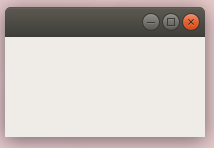
\includegraphics[width=.3\textwidth]{images/Chapter_08/01_simple_window.png}
\end{center}

The style matches the operating system where it runs. It is a simple, empty window. However, we can already start understanding how Qt works. A user interface is a program that keeps running in a loop. When we click and drag to resize a window, for example, there is always a program responsible for knowing how to do it. In Qt, this never-ending loop is the \texttt{QApplication}. Whatever window we want to create needs to belong to an application, and that is why the first thing we did was defining \texttt{app}.

In the following line, we define a new object, called \texttt{win}, which is a \texttt{QMainWindow}. As the name suggests, the main windows are the core of the user interface. From the main window, we can open dialogs, other windows, but the main window is central to our program. After creating it, we show it. The last line is where the application loop starts. The \texttt{app.exec()} command is blocking. Therefore nothing that comes after is executed until we finish with the user interface.

\exercise{To understand a bit better what is going on with the user interface, you are encouraged to try different things. For example, what happens if you don't show the window or add a few print statements to see when they get executed. You can also try to define the window before the application.}

Having an empty window is not particularly useful, so we can start adding elements to it. First, we add a title to the window, like this:

\begin{minted}{python}
    win.setWindowTitle('My First Window')
\end{minted}

Very slowly, our program starts taking shape and looking more professional. We can also add an interactive element, such as a button. We can define one like this:

\begin{minted}{python}
    from PyQt5.QtWidgets import QApplication, QMainWindow, QPushButton

    app = QApplication([])
    win = QMainWindow()
    win.setWindowTitle('My First Window')
    button = QPushButton('Press Me', win)
    win.show()
    app.exec()
\end{minted}

Which will produce a small window, like this:

\begin{center}
    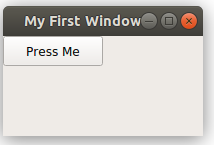
\includegraphics[width=.3\textwidth]{images/Chapter_08/02_simple_window_and_button.png}
\end{center}

Notice that when we defined the button, we added a second argument, \texttt{win}. Qt has a hierarchical structure, where each element is called a \emph{widget}. We have imported three widgets so far: the application, the window, and the button. All widgets live inside the application loop, but we have to establish the relationship between them. By passing the window as the second argument, we are explicitly saying that the button belongs to the window.

\exercise{Remove the \texttt{win} from the definition of the button, and see what happens}
\exercise{Alter the order and make the button the parent of the main window, does this work?}

A big part of working with Qt is finding out how to relate different widgets to each other, how to position them. \texttt{QMainWindows} are special because they must hold widgets within them. That is why they specify a method to determine which Widget is the most important for the window, or in Qt jargon, which Widget is the central Widget. We can explicitly declare it:

\begin{minted}{python}
    button = QPushButton('Press Me')
    win.setCentralWidget(button)
\end{minted}

We removed the \texttt{win} from the declaration of the button, but if it's there it doesn't change the behavior. The window now looks somewhat different:

\begin{center}
    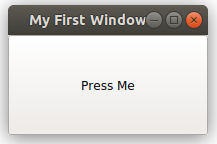
\includegraphics[width=.3\textwidth]{images/Chapter_08/03_simple_window_and_central_widget.png}
\end{center}

You can try resizing the window, and you see that the button scales. By declaring the button as the central Widget of the window, we made the relationship even stronger. The last possibility which is worth mentioning before moving forward is that we can also show the button independently from the window, like this:

\begin{minted}{python}
    win.setWindowTitle('My First Window')
    button = QPushButton('Press Me')
    win.show()
    button.show()
\end{minted}

In this case, the window and the button are two independent components, like we show in the image below. For the program to finish, we must close both the button and the window.

\begin{center}
    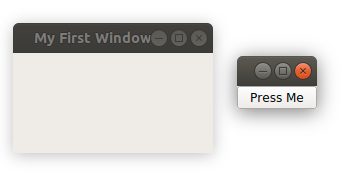
\includegraphics[width=.3\textwidth]{images/Chapter_08/04_window_button_separated.png}
\end{center}

Qt offers a great deal of flexibility, which doesn't mean we need actually to use it. Having buttons floating around the screen does not sound like a good idea, but it is a possibility in case we ever need it.

Now that we have a button on a window, we are craving to do something with it.


\section{Signals and Slots}\label{sec:signals-slots}
Qt offers a programming pattern known as \emph{Signals} and \emph{Slots}. The core idea is that different actions on a user interface trigger a signal. For example, moving the mouse over an element triggers a signal. This signal is then caught by \emph{slots}, which do something with the information provided. When we move the mouse over a button (this is also knowns as hovering), its background changes color. It is a clear example of the signal/slot paradigm.

Every Widget that we can place on screen has a myriad of signals. From interactions with the mouse to changes in shape or size triggered by reshaping the window, to time-based signals. It does not mean we need to know them all, nor that we use them all. But once we understand the pattern, we know where to go and find what we are after. The button has one signal called, very eloquently, \texttt{clicked}. To use it, we must define a function that can be called every time the signal fires. This function is the \emph{slot}. We can expand our example code like this:

%! Suppress = Ellipsis
\begin{minted}{python}
    def button_clicked():
    print('Button Clicked')

    [...]
    button = QPushButton('Press Me')
    button.clicked.connect(button_clicked)
    win.setCentralWidget(button)
\end{minted}

We can see that every time we click the button, the program prints a message to the screen. It is very important to note that we used \texttt{button\_clicked} and not \texttt{button\_clicked()}. It is the same that we discussed in Section~\ref{subsection: multithreading} when discussing multithreading. We must use the function itself as a slot, and not the outcome of the function.

\subsection{Start a Scan}\label{subsec:start-scan-gui}
With what we have done so far, triggering a scan from the user interface becomes almost trivial. For the time being, we can keep working on the \emph{Examples} folder, but this time let's create a new file called \textbf{start\_gui.py}. We only need that when we press the button, a scan starts. We need to mix what we already have in \textbf{start\_experiment.py} with what we have done above. It can look like this:

\begin{minted}{python}
    from PyQt5.QtWidgets import QApplication, QMainWindow, QPushButton

    from PythonForTheLab.Model import Experiment

    experiment = Experiment('experiment.yml')
    experiment.load_config()
    experiment.load_daq()

    app = QApplication([])
    win = QMainWindow()
    win.setWindowTitle('My First Window')
    button = QPushButton('Start Scan')

    button.clicked.connect(experiment.do_scan)

    win.setCentralWidget(button)
    win.show()
    app.exec()

    experiment.finalize()
\end{minted}

The code above is a merge between what we did in the previous chapter and this one. We define the experiment as always, and the window and button as we have just learned. However, the line that does all the magic is this one:

\begin{minted}{python}
    button.clicked.connect(experiment.do_scan)
\end{minted}

We can try the program. When we click the button, a scan starts. However, there is something else happening. The window freezes, we are not able to reshape it, close it. In some cases, especially on Windows, the program crashes, and we get a message saying whether we want to report the issue.

\exercise{Can you guess why the window freezes?}

When we described the flow of a Qt program, we talked about a loop taking care of the interactions within the program. However, if we trigger a scan using \texttt{do\_scan}, we are going to block that loop. Both Qt and Python are single-threaded applications by default, and when one blocks, the other blocks as well. And by talking about single-threaded applications, we gave a hint to how this can be solved.

At the end of the last chapter, we developed a different method called \texttt{start\_scan} that creates a separate thread to hold the scanning, effectively releasing the main thread to do other tasks. We can change just one line of code and achieve a very different behavior:

\begin{minted}{python}
    button.clicked.connect(experiment.start_scan)
\end{minted}

We have developed a somewhat functional program. We have a window with a button from which we can control our experiment. It is already quite an excellent achievement. We also got some extra features out of the box, such as preventing the user from triggering two scans at the same time.

Sometimes, the easiness of developing this kind of solution misguides the readers. It was so easy to achieve what we achieved so far because we spent a lot of time and effort developing a proper \emph{experiment class}. The threading, the checks to prevent two scans, and some extra things that keep appearing in this and next chapter are thanks to a well-designed model.


\section{Extending the Main Window}\label{sec:extending-main-window}
We have seen how to get started by creating the main window and adding a button to it. However, we can also start seeing that if we try to add more elements, the code is going to become more and more convoluted. It would be a nice addition if the window we design here could be used for different purposes as well. As we have already seen many times, a good idea when we want to make blocks of code reusable is to convert them into classes. Qt is ideally suited for this because every Widget they provide is an object with a special inheritance tree.

In the folder \emph{View} we can create a file called \textbf{main\_window.py}, and we can add the following code:

\begin{minted}{python}
    from PyQt5.QtWidgets import QMainWindow


    class MainWindow(QMainWindow):
        def __init__(self):
            super().__init__()
            self.setWindowTitle('My First Window')
\end{minted}

Before discussing what we have done, we can quickly go back to \textbf{start\_gui.py} and change the following two lines of code:

\begin{minted}{python}
    win = QMainWindow()
    win.setWindowTitle('My First Window')
\end{minted}

with this one:

\begin{minted}{python}
    win = MainWindow()
\end{minted}

We should also remember to change the imports at the top of the file by these:

\begin{minted}{python}
    from PyQt5.QtWidgets import QApplication
    from PythonForTheLab.View.main_window import MainWindow
\end{minted}

If we run the code, we see that it behaves as it was behaving previously. In our code, we create a new class called \texttt{MainWindow}, which in turn inherits from \texttt{QMainWindow}. It is always important to call \texttt{super()} because that runs the init method from the QMainWindow itself, setting up all the parameters, signals, properties that we need to generate a window. There is, however, a difference with a plan \texttt{QMainWindow}, we specify its title. Effectively, we have now extended the pure \texttt{QMainWindow} class to include a title by default.

\note{It is a personal preference when I start developing a program that has only one main window to name it \texttt{MainWindow}, removing the preceding \texttt{Q}. It can lead to mistakes if we overlook the small difference in both names. Depending on taste, an alternative is to call the windows by what they are supposed to do, such as \texttt{ScanWindow}. It depends on the reader's preferences.}

We can add the button, and the slot, like this:

\begin{minted}{python}
from PyQt5.QtWidgets import QMainWindow, QPushButton


class MainWindow(QMainWindow):
    def __init__(self, parent=None):
        super().__init__(parent=parent)
        self.setWindowTitle('My First Window')
        self.button = QPushButton('Press Me')
        self.setCentralWidget(self.button)

        self.button.clicked.connect(self.button_clicked)

    def button_clicked(self):
        print('Button Clicked')
\end{minted}

We can test this code again and see that we have recovered what we had before. Every time we press on the button, a message appears on the screen. We can also go one step further and start thinking about how to work with the experiment itself. The window is not aware of any experiments, but we would like to be able to trigger a scan if we press the button. Therefore, the experiment has to come from outside of the class and be stored within.

We have already done something like this. When we developed the driver in Section~\ref{section:going-higher-level}, we could send the port number to the class through the \texttt{\_\_init\_\_} method. We did the same for the device model in Section~\ref{section:device-model}, and for the experiment model in Section~\ref{section:skeleton-experiment-model}. In all those cases, we were using simple strings, but we are not limited to them. Arguments of methods, or any function for the matter, can be complex objects as well.

We can adapt the \texttt{MainWindow} to accept an experiment as argument, store it as an attribute and use it when we need to. The code would look like this:

\begin{minted}{python}
    [...]
    class MainWindow(QMainWindow):
        def __init__(self, experiment=None):
            super().__init__()
            self.experiment = experiment

            [...]
        def button_clicked(self):
            self.experiment.start_scan()
            print('Scan Started')
\end{minted}

The changes to the code were minimal but significant. We have included \texttt{experiment=None} in the init. We have provided a default value for the experiment because this allows us to run the program even if we have no experiment defined. It is useful if we want to test how the window looks like quickly. However, as soon as we press the button, the program crashes. We have to update the \textbf{start\_gui.py} script to accommodate for the changes:

\begin{minted}{python}
experiment = Experiment()
experiment.load_config('experiment.yml')
experiment.initialize()

app = QApplication([])
window = MainWindow(experiment)
window.show()
app.exec()

experiment.finalize()
\end{minted}

We pass \texttt{experiment} directly to the window, and it takes care of the rest. We can now safely trigger a scan from the user interface. What is important to note is that once we reach this step, all the rest happens directly on the view. The script that we use to open the window stays unaltered. Even in much more complex programs, we use the same pattern\footnote{See, for example, how PyNTA starts its user interface: https://bit.ly/WindowExperiment}.

\section{Adding Layouts}\label{sec:adding-layouts}
So far, our window holds only one button, and we set that button to be the central Widget of the window. This makes it virtually impossible to add any other button or object. Therefore, it is time to start sophisticating our user interface\footnote{In this chapter we decided to go lower level, programming every feature, but in the next chapter we will see how to do it with the QtDesigner software, which will speed up the process}. The basic building blocks in Qt are \texttt{QWidgets}, and Qt allows us to place widgets inside of widgets at our will. We also know that Main Windows require a central widget. Therefore, we can create a widget that holds two buttons: start and stop, and that Widget is the central Widget of the window. We use this opportunity to clean up the names we have used, to make them more descriptive as well, it is important to pay attention to all the changes made:

\begin{minted}{python}
from PyQt5.QtWidgets import QMainWindow, QPushButton, QWidget


class MainWindow(QMainWindow):
    def __init__(self, experiment=None):
        super().__init__()
        self.experiment = experiment
        self.setWindowTitle('Scan Window')

        self.button_widgets = QWidget()
        self.start_button = QPushButton('Start', self.button_widgets)
        self.stop_button = QPushButton('Stop', self.button_widgets)

        self.setCentralWidget(self.button_widgets)

        self.start_button.clicked.connect(self.start_scan)

    def start_scan(self):
        self.experiment.start_scan()
        print('Scan Started')
\end{minted}

If we run the program again, we will see a Window like the one below:

\begin{center}
    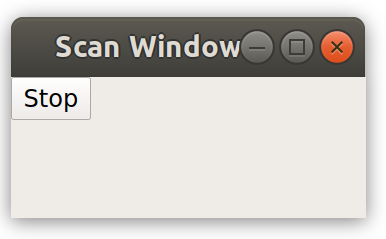
\includegraphics[width=.3\textwidth]{images/Chapter_08/05_window_without_layout.png}
\end{center}

The stop button is visible, but not the start button. It happens because Qt has no way of knowing where we want to add the buttons and place them in the same position. The one that gets added later is on top.

\exercise{Change the order in which we define the buttons and see that one or the other gets on top. If the button that is below has a much longer text, you can see it beneath the top one.}

We could specify explicit coordinates for the positions of the buttons, but there is a much simpler approach using layouts. In Qt, there are 4 basic layout types: Horizontal, Vertical, Grid, and Form. With the first two, each time we add a widget, it is added either below or to the right. With the grid layout, we can control the position, width, and height based on a grid we define. The form defines two columns, ideally to hold some labels and inputs. We see more about layouts in the following chapter. For the time being, if we want to add two buttons, we can choose a horizontal layout. The code of the \texttt{MainWindow} takes a few extra lines to set everything up properly:

\begin{minted}{python}
from PyQt5.QtWidgets import QHBoxLayout
[...]
self.button_widgets = QWidget()
self.start_button = QPushButton('Start')
self.stop_button = QPushButton('Stop')
layout = QHBoxLayout(self.button_widgets)
layout.addWidget(self.start_button)
layout.addWidget(self.stop_button)

self.setCentralWidget(self.button_widgets)
\end{minted}

In Qt, the horizontal layout is called \texttt{QHBoxLayout}, and we apply it to the \texttt{buttons\_widget}. Then, we add the start and stop to the layout, instead of directly to the widget. This window will look much better:

\begin{center}
    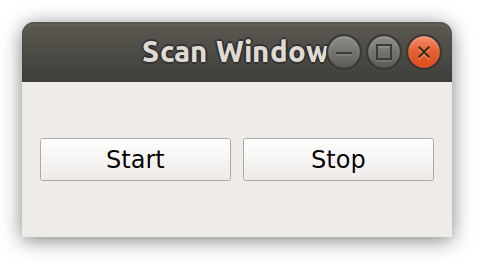
\includegraphics[width=.3\textwidth]{images/Chapter_08/06_window_with_layout.png}
\end{center}

If we resize it, we see that the buttons take the entire width, and they are always centered. It is already a good improvement compared to the simple window with which we started. Before we finish this section, these two exercises are a good way of practicing the skills acquired so far:

\exercise{Change \texttt{QHBoxLayout} by \texttt{QVBoxLayout} to see the buttons stacked vertically.}

\exercise{Connect the stop button to a method that stops the scan}

\section{Plotting Data}\label{sec:plotting-data}
We finish this section by adding a plot of the data in real-time. We already did something similar in Section~\ref{sec:basic-plotting}. Parts of the code are very similar. Our window slowly starts getting more complex, with more elements. So far, we have two buttons stacked horizontally, but we would like to show the plot beneath the buttons, not next to them. One of the most natural solutions is to start stacking widgets, instead of making the \texttt{buttons\_widget} the central Widget, we can make another one that contains the buttons and the plot.

\begin{minted}{python}
import pyqtgraph as pg
from PyQt5.QtWidgets import (QMainWindow,
                             QPushButton,
                             QWidget,
                             QHBoxLayout,
                             QVBoxLayout, )

class MainWindow(QMainWindow):
    def __init__(self, experiment=None):
        super().__init__()
        self.experiment = experiment
        self.setWindowTitle('Scan Window')

        self.central_widget = QWidget()
        self.button_widgets = QWidget()
        self.start_button = QPushButton('Start')
        self.stop_button = QPushButton('Stop')
        self.plot_widget = pg.PlotWidget(title="Plotting I vs V")
        self.plot = self.plot_widget([0], [0])

        layout = QHBoxLayout(self.button_widgets)
        layout.addWidget(self.start_button)
        layout.addWidget(self.stop_button)

        central_layout = QVBoxLayout(self.central_widget)
        central_layout.addWidget(self.button_widgets)
        central_layout.addWidget(self.plot_widget)

        self.setCentralWidget(self.central_widget)
\end{minted}

Some remarks about the code before we run it. We are using \texttt{()} for the import because it makes it easier to stack the modules instead of having a very long line that becomes hard to read. In the window, we define three widgets now, \texttt{central\_widget}, \texttt{button\_widgets}, and \texttt{plot\_widget}. The plot widget is very similar to what we did in the previous chapter. The only difference is that we store the Widget itself and the plot separately, and we explain why later. We didn't touch the buttons, but instead of adding them as the central Widget, we add them to a higher-order widget. By stacking the buttons horizontally between themselves, but vertically to the plot, we get a window that looks like this:

\begin{center}
    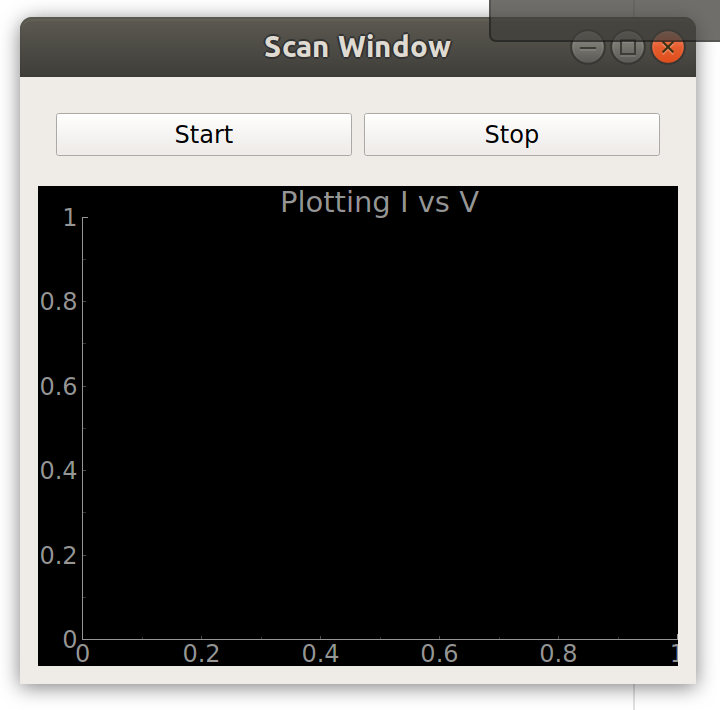
\includegraphics[width=.4\textwidth]{images/Chapter_08/07_window_empty_plot.png}
\end{center}

We are halfway through with what we wanted. If we resize the window, the plot changes, taking all the space available, even if we expand the window vertically, there is no gray area around the buttons. How the surrounding elements control the shape of a widget is one of the properties that can be specified.

\note{We make several remarks about possibilities with Qt that we don't explore further. We just want to point out that every single thing that happens on a user interface was decided, and can be changed. Not only the aspect, such as colors but also how different elements relate to each other and change shapes when the container window changes.}

To plot the data we acquire, we just need to update the plot periodically. Qt offers a special object called \texttt{QTimer} that also specifies signals. With timers, we can trigger periodic actions without interrupting the rest of the program. We also need to develop a method that can update the plot. The Main Window code looks like this:

\begin{minted}{python}
    from PyQt5.QtCore import QTimer
    [...]

    class MainWindow(QMainWindow):
        def __init__(self, experiment=None):
            [...]
            self.timer = QTimer()
            self.timer.timeout.connect(self.update_plot)
            self.timer.start(50)

        def update_plot(self):
            self.plot.setData(self.experiment.scan_range, self.experiment.scan_data)
\end{minted}

The timer is relatively easy to understand. It is an object that triggers a signal, \texttt{timeout} periodically. We connect that signal to the method \texttt{update\_plot}. When we start the timer, we need to specify the time interval in milliseconds, therefore $50\,\textrm{ms}$ means a refresh rate of $20\,\textrm{Hz}$. The \texttt{update\_plot} method is different from what we did in the previous chapter. Instead of using \texttt{plot}, we are using \texttt{setData}. There are two reasons for it. First, if we use \texttt{plot()}, we create a new plot on top of the existing one. We wouldn't be refreshing the data but drawing on top of it. After a while, especially if the parameters or results change, we would see several lines overlapping. The second reason is speed. \texttt{plot()} is a relatively slow method because several things need to be set up, such as the axes, labels, ticks. By using \texttt{setData} PyQtGraph automatically reuses the elements available.

However, if we try to run the code, we will get a problem:

\begin{minted}{bash}
    AttributeError: 'Experiment' object has no attribute 'scan_range'
\end{minted}

\exercise{Find out why are we getting this error even though we didn't find it when running a more straightforward script in the previous chapter}

When the window starts, we automatically start the timer, which, in turn, tries to update the plot. However, the experiment class does not have any \texttt{scan\_range} nor \texttt{scan\_data} until the experiment starts running. A bypass to the problem would be to start the timer after we have started the scan, but this is very unreliable. Best-practices in Python indicate that we should always define attributes in classes in the \texttt{\_\_init\_\_} method. It means that as soon as we create the object, the attributes exist, even if with place-holder values.

When we developed the \emph{Experiment class}, we completely neglected this practice. We added \texttt{self.} whenever we needed to have data available through the class and also from outside of it. We leave the definition of most of the attributes to the reader, but we show how to solve the problem with the scan. Going back to the experiment model, we need to add the following:

\begin{minted}{python}
    class Experiment:
        def __init__(self, config_file):
            [...]
            self.scan_range = np.array([0]) * Q_('V')
            self.scan_data = np.array([0])  * Q_('V')
\end{minted}

We decided to define both attributes as numpy arrays holding only one value: $0\,\textrm{V}$. If we try to plot these results, we get a single point at the origin. It may raise other questions, such as whether it is better to have a $0$ or a \texttt{None} value, because $0\,\textrm{V}$ could be a valid measured value. It is left to the sensitivity of the reader to judge what is best in their specific case. For our purposes, this is enough to get the window running and showing a plot of the data in real-time once the scan starts.

\exercise{Every attribute in any class should be defined in the init of that class. Go through all the models, and see whether there are attributes used but not defined at instantiation.}

\subsection{Refresh Rate and Number of Data Points}\label{subsec:refresh-rate-and-number-of-data-points}
When we follow the strategy of using a timer for refreshing the plot, we can be tempted to increase the refresh rate to make the animations more appealing, but we have to be careful with this. On the one hand, if we are generating data at, let's say, $1\,\textrm{Hz}$, doesn't matter how fast we refresh the plot, it won't change faster than once per second.

Let's assume we are acquiring data much faster than once per second, perhaps at hundreds or thousands of new points per second. We have to consider how fast the screen of the computer can redraw the elements on it. Most screens work at $30\,\textrm{Hz}$, some may go to $60\,\textrm{Hz}$. Therefore, if we try to update the plot faster than that, we just waste computer power on something that the screen never can show us.

There is one additional limitation that is our own eyes. We can't process images faster than at 30fps. Already at $50\,\textrm{Hz}$, we don't see the lights in our room blinking. If we are not interested in video quality for the update of our plots, we can safely go down to $20\,\textrm{Hz}$, and the images still look fluid.

\exercise{Instead of plotting data from the device, you can update the plot with points that oscillate in time and see up to which point the refresh rate affects the quality of what you are showing.}

There is one more thing to consider beyond the refresh rate, which is the number of points we are plotting. Most screens have a few thousand pixels in each direction. A very common resolution is $1920\times1440\,\textrm{pixels}$. If we acquire $10000$ data points and try to show them on the screen, they have to be reduced almost 5 times to fit the number of pixels available on the screen. In this reduction process, we can lose many details. If we use downsampling, for example, and we are looking for a narrow peak, the chances of it appearing on the image can be very little.

We have to be aware of the number of data pixels that we try to show not only on user interfaces but also when we are preparing plots for printing or inserting into a PDF. The number of dots a printer can generate is normally specified as dots per inch, or dpi. Even at $600\,\textrm{dpi}$, an image with a width of $8\,\textrm{cm}$ (standard 1-column figure on a paper) will have under 2000 dots in its horizontal direction. And, of course, a reader behind a computer screen is limited to its pixels.

\section{Conclusions}\label{sec:basic-gui-conclusions}
In this chapter, we have started building a user interface for the experiment. We explored how to get started with Qt, PyQt, how to use buttons to trigger actions using signals and slots. We also saw how to connect a basic user interface to the experiment model. It showed us the advantages of having an experiment that already runs measurements in its threads.

We also saw how to extend the basic building blocks of Qt, such as QMainWindow, by subclassing it and adding the elements we needed. We saw how to build widgets with more widgets inside, how to lay them out on more complex patterns. Finally, we added simple plotting capabilities to the window, refreshing whatever data the experiment is acquiring in real-time.

This chapter typically generates much satisfaction for people who are developing user interfaces for the first time. On the other hand, we have done much work, and we got a window that does not look nearly as nice as the windows with which we are familiar from other programs. On the one hand, this helps us understand how much effort is behind every window we see. On the other, it pushes us to go one step further.

In the next chapter, we start seeing how to improve the design of our User Interfaces by using a program called Qt Designer.

    \chapter{User Input and Designing}\label{ch:user-input-designer}

\section{Introduction}\label{sec:user-input-introduction}
You started building a GUI by programming every aspect of the interface. You built a \py{MainWindow} class, added some buttons and a plot. A logical next step would be to add a way to change the parameters that build up the scan. You would like to be able to change the \py{start}, \py{stop}, and \py{num_points} values directly from the user interface and not from a config file that gets read-only at the beginning.

You could continue adding elements to the program as you did in the previous chapter, but that is time-consuming. In this chapter, you're going to introduce a program called \textbf{Qt Designer} that is targeted precisely at speeding up the design of user interfaces. You see not only how to make the program better looking, but you're also going to see what happens when you let users input data, what problems may arise, and you show the way to keep improving based on what you achieve by the end of the chapter.

\section{Getting Started with Qt Designer}\label{sec:getting-started-with-qt-designer}
You explained how to install Qt Designer in Section~\ref{sec:install-qt-designer}. Different operating systems and different Python versions have a slightly different way of opening the program.

If you're using \textbf{Anaconda on Windows}, you only have to open the start menu and type \textit{Designer}, press \py{}enter once it finds it. \textbf{Anaconda on Linux} is similar, open a terminal, either from the base environment or the environment used for this book, type \py{designer}, press enter, and a window should open.

If you're using \textbf{plain Python on Windows}, and you installed \py{pyqt5-tools}, you only need to start the \emph{Command Prompt}, activate the environment where you work, type \py{designer.exe}, and press enter. If you're using \textbf{plain Python on Linux}, you installed the Designer as part of the package \py{qttools5-dev-tools}. In this case, the Designer is an actual application that you can find within the installed apps in your distribution.

The Designer welcomes us with a screen like the one below. In between the template/forms options, you can already see two familiar options: Widget and Main Window.

\begin{center}
    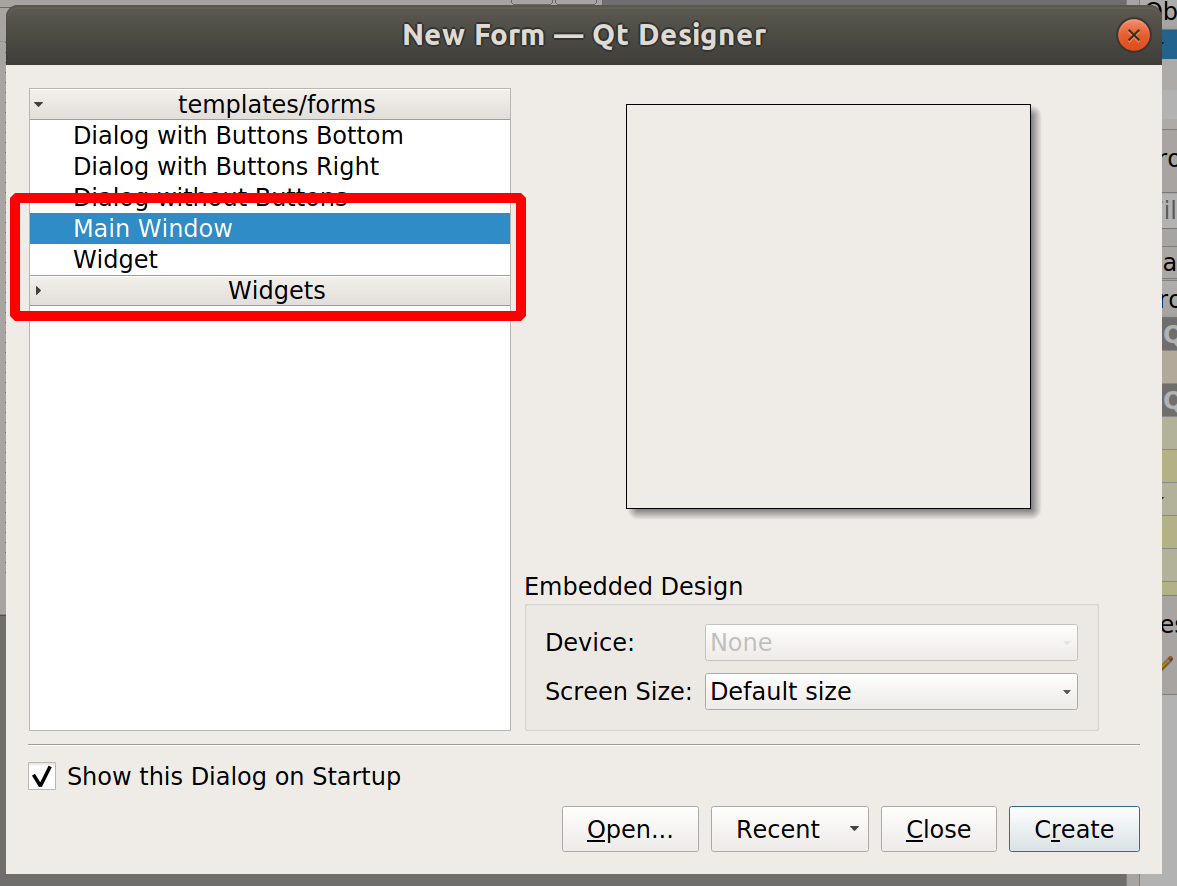
\includegraphics[width=.5\textwidth]{images/Chapter_09/01_Designer_Welcome.png}
\end{center}

You start by recreating the window you developed in the previous chapter. You start by selecting \textbf{Main Window}, and clicking create. The Designer opens the working area with an empty main window. That space is our canvas to start adding elements. In the previous chapter, you created a central widget explicitly. The Designer already did this for us. You can see it on the object inspector at the right sidebar:

\begin{center}
    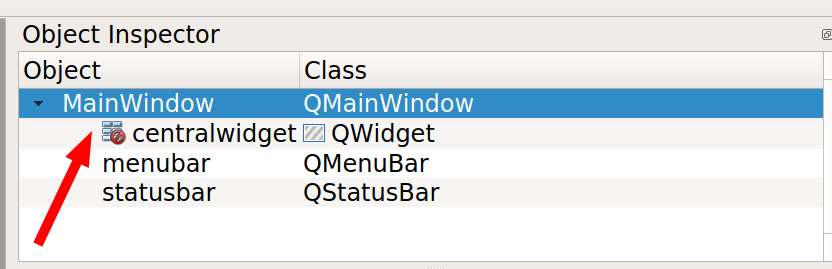
\includegraphics[width=.5\textwidth]{images/Chapter_09/02_central_widget.png}
\end{center}

Note that the Designer named the central widget \py{centralWidget} instead of \py{central_widget}. Naming classes, variables, methods, and functions is completely free in Python, but some conventions make code easier to understand at first sight. One is naming classes with the Camel Case convention, such as \py{MainWindow}, and attributes in lower-case with words separated by underscores. You can change the name of the central widget by clicking on it and changing the \py{objectName} name property:

\begin{center}
    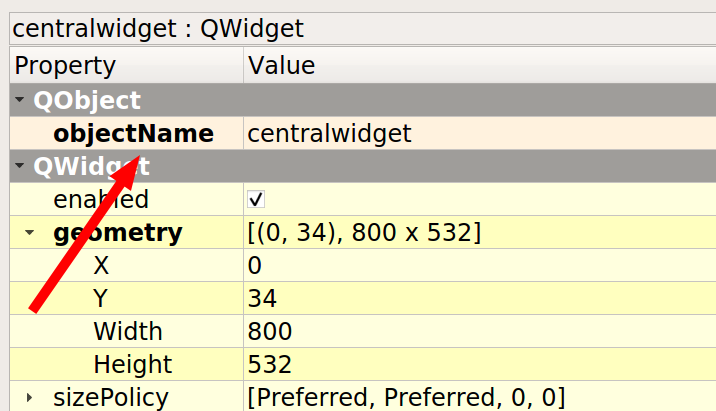
\includegraphics[width=.5\textwidth]{images/Chapter_09/03_central_widget_name.png}
\end{center}

Now you've the central widget with the same name you used in our Python class. You can add the buttons widget by dragging and dropping an empty widget to the window, that can be found in the containers group of elements. After you add the widget, you can also see it appears in the object inspector on the right sidebar. You can change its name to \py{button_widgets}.

\begin{minipage}{0.45\linewidth}
    \centering
    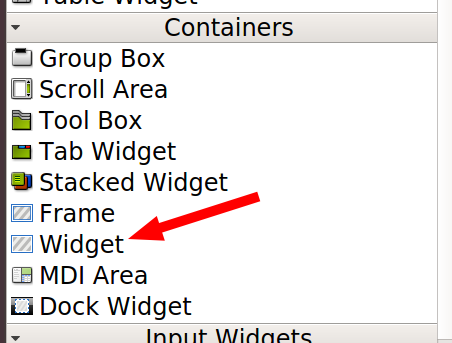
\includegraphics[width=\textwidth]{images/Chapter_09/04_empty_widget.png}
\end{minipage}
\hspace{0.5cm}
\begin{minipage}{0.45\linewidth}
    \centering
    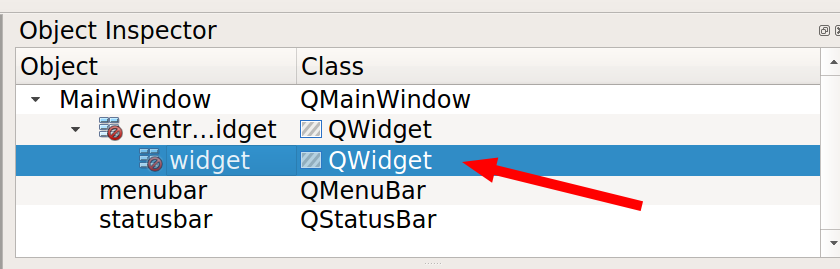
\includegraphics[width=\textwidth]{images/Chapter_09/04_empty_widget_structure.png}
\end{minipage}

To add the start and stop buttons, you can just drag and drop two \py{QPushButton}s to the window. You've to be sure you drop them inside the buttons widget you created earlier. To change the text that appears on the button, you can double click on it and edit the text. You can make one button with the text \emph{Start}, and the other with the text \emph{Stop}. The text on the button is not the name of it. You must change the name of the buttons, and to repeat the same structure of the previous chapter, you're going to call them \py{start_button} and \py{stop_button}. The window and the structure should look like this:

\begin{minipage}{0.45\linewidth}
    \centering
    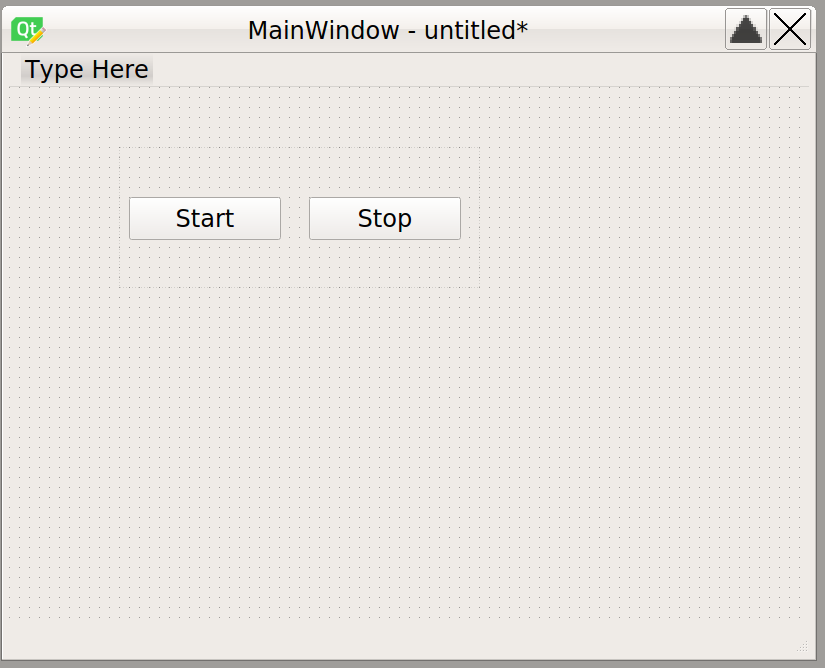
\includegraphics[width=\textwidth]{images/Chapter_09/05_main_window_buttons.png}
\end{minipage}
\hspace{0.5cm}
\begin{minipage}{0.45\linewidth}
    \centering
    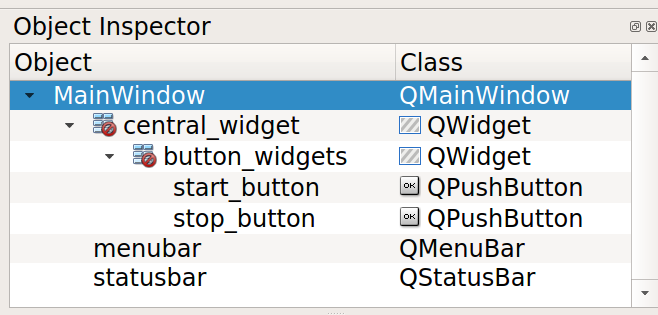
\includegraphics[width=\textwidth]{images/Chapter_09/05_main_window_structure.png}
\end{minipage}

\infoInfo{Screenshots}{Explaining how to use a designing program through screen captures requires much patience from the reader. You try to highlight the checkpoints that allow comparing what the reader does with what you show here. Practice and a critical view is the best that can the reader can do at this stage.}

You've a window with the buttons, but you're missing the layout to make it look as good as you had in the previous chapter. The Designer has a toolbar dedicated exclusively to the layouts; you can find it at the top of the main window space; it looks like this:

\begin{center}
    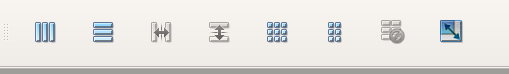
\includegraphics[width=.4\textwidth]{images/Chapter_09/06_layouts.png}
\end{center}

To apply a layout to a widget, you can click first on the widget inside the Object Inspector and then click on the desired layout. You can apply a vertical layout to the \py{central_widget} and a horizontal layout to the \py{button_widgets}. When you apply a layout to widgets, it shows as a different icon on the Object Inspector.

\begin{center}
    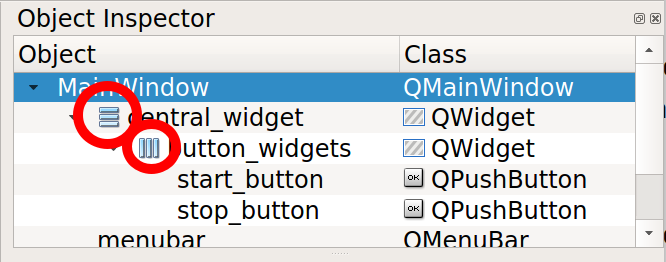
\includegraphics[width=.4\textwidth]{images/Chapter_09/07_widgets_with_layouts.png}
\end{center}

You're ready to save the window. Let's create a new folder called \textbf{GUI} inside the \emph{View} folder, and you can call the file \py{main_window.ui}. Once you save the designer file, you're ready to go back to Python to use this window. You can go back to \textbf{main\_window.py}, and you can start editing the \py{MainWindow} class. Since some of the elements are now defined directly on the designer file, you remove them from the class:

%! Suppress = Ellipsis
\begin{minted}{python}
    import os
    from PyQt5 import uic
    [...]

    class MainWindow(QMainWindow):
        def __init__(self, experiment=None):
            super().__init__()

            base_dir = os.path.dirname(os.path.abspath(__file__))
            ui_file = os.path.join(base_dir, 'GUI', 'main_window.ui')
            uic.loadUi(ui_file, self)

            self.experiment = experiment

            self.plot_widget = pg.PlotWidget()
            self.plot = self.plot_widget.plot([0], [0])
            layout = self.central_widget.layout()
            layout.addWidget(self.plot_widget)
    [...]
\end{minted}

Besides the new imports, the fundamental change to the \py{MainWindow} class is that you load the file using \py{uic.loadUi}. When you try to import files in Python, you always have to be careful with determining the path from which you're importing. You already encountered the syntax of \py{dirname} when you were adding the root folder to the path in Section~\ref{sec:appending-path}. The idea is the same, but you're interested in the folder where the current Python file is located.

The command \py{uic.loadUi} takes two arguments; the first is the file you want to load, and the second is the object to which it's applied. You use the \py{self} to indicate that you want to apply the layout to the entire \py{MainWindow}. If you develop a more modular program, such as defining individual widgets, you could apply the Designer file just to the widget in which you're interested.

The rest of the window stays the same. You only removed the definition of \py{central_widget} and the buttons. Since you've the layout of the central widget specified in the Designer, you need to access it to be able to append the plot widget. It's what this line is doing:

\mint{python}{layout = self.central_widget.layout()}

You can go ahead and run the program, and you see that the window appears as it did before, without changes, even though you're now pulling the elements from the Designer file.

\subsection{Deciding whether or not to compile UI files}\label{subsec:compiling-or-not-compiling-ui-files}
Most tutorials online add one step after creating the Designer's file. They normally suggest transforming the \py{.ui} files into a \py{.py} file. There's a program able to do it for us, that can be triggered from the command line:

\begin{minted}{bash}
    pyuic5 main_window.ui -o compiled_window.py
\end{minted}

You can explore both files and see the differences. If you open the \emph{ui} file with a text editor, you find out it's plain text and formatted following a standard called \emph{XML}, or extended markup language. This format is very similar to how websites are built, \emph{HTML} stands for hypertext markup language. Going through the file, you find the place where you defined the buttons, surrounded by some more information, such as the layout, and the text of the button.

If you open the generated Python file, you find the same information but formatted in the same way you've done it in the previous chapter. You can go to the declaration of the start button, and you find a line almost identical to the one you used in the previous chapter

\mint{python}{self.start_button = QtWidgets.QPushButton(self.button_widget)}

The question is whether you \textbf{need} to compile the \emph{ui} files to Python files or not. Qt was developed with C++ programmers in mind, and for a C++ program, it's essential to have each variable defined with a specific type before compiling the code. Qt offers a program, \py{uic} to transform \emph{ui} files to \emph{C++} compatible files. Most Python tutorials built on that experience and kept the recommendation. But for Python, this step is not necessary at all.

There's one caveat, however. If you don't transform the file to a Python file, editors won't be able to know which attributes are available on the windows and widgets. The editor won't have any idea whether there's a \py{start_button} or not defined. It means that to be sure, you should keep opening the designer program and see how you named the buttons and elements. But this is the only drawback that non-compiling has.

In our experience, modifying the designer files and seeing the changes as soon as you restart the program outweighs the problems of not being able to auto-complete. If you're systematic with the naming conventions, you won't face many issues. And if you do encounter issues with attributes not defined, you know that the root of the problem is that you used one name in the Designer and a different one in Python.

\section{Adding User Input}\label{sec:adding-user-input}
\begin{center}
    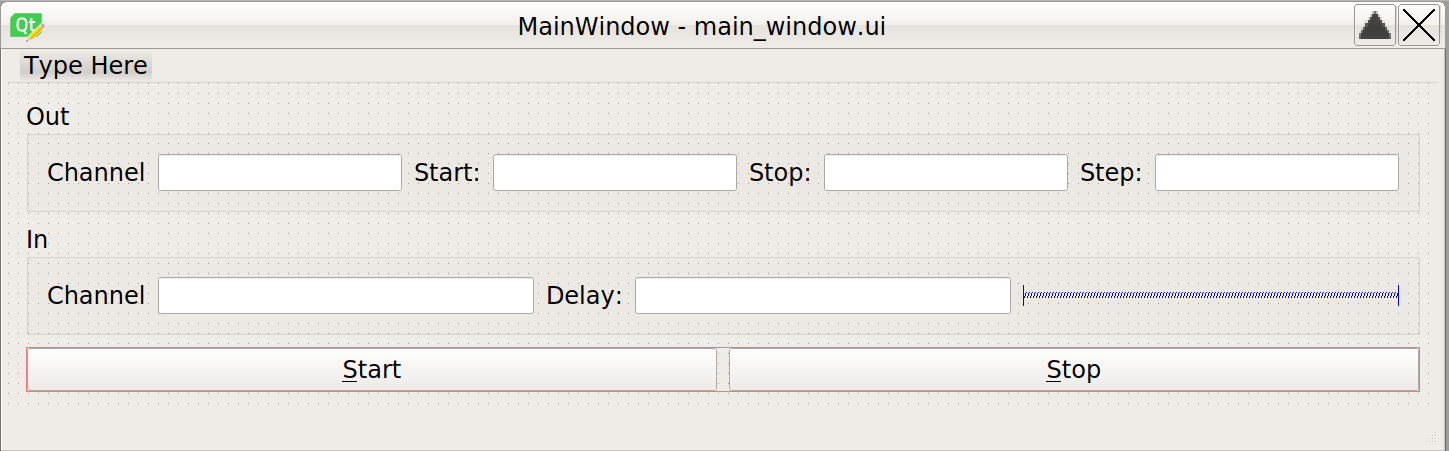
\includegraphics[width=.5\textwidth]{images/Chapter_09/08_final_window_example.png}
\end{center}

It's time to bring our program to the next level by adding the possibility of entering the values of the scan before triggering it. The goal is to have a window that looks like the image above. You structured the window in three rows, one for selecting the range of the scan and the channel, one for the input and delay between points and finally the buttons. Below it, you append the plot, as you've done before.

First, you start by designing the window. You do not cover every single detail as you did in the previous section, because it would become too cumbersome to follow. Therefore you leave to the discretion of the reader whether they want to try it by themselves or get the designer file from the online repository. The easiest way to reproduce the window is by looking at the structure you should obtain after placing all the elements:

\begin{center}
    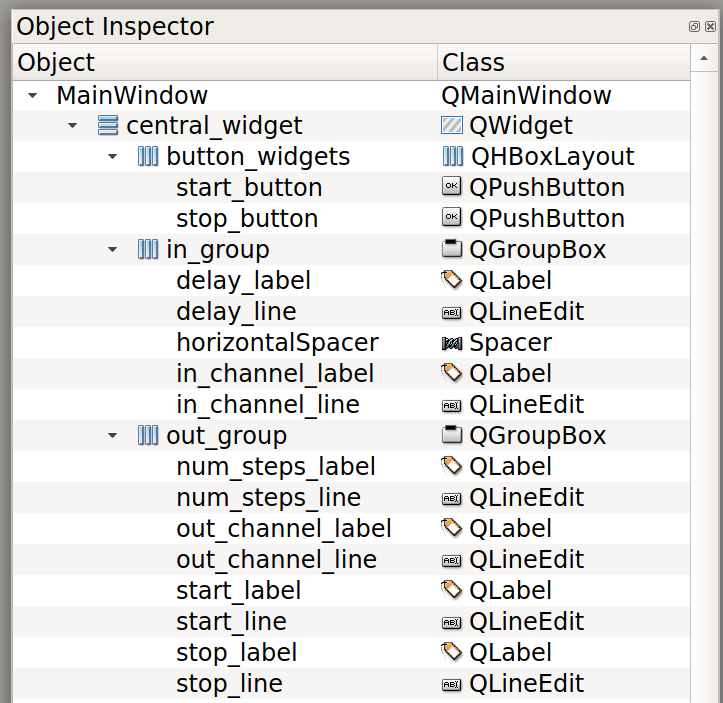
\includegraphics[width=.5\textwidth]{images/Chapter_09/09_final_window_structure.png}
\end{center}

The central widget and the buttons are there, as always, but you added two more widgets now, they are of a particular type called \py{QGroupBox}, meant for grouping elements together. They also have a title that appears at the top left, and become quite handy to understand what you need to edit before starting a scan To handle input from the user, you chose \py{QLineEdit} widgets. These widgets allow the user to input any type of text, precisely as you need.

The rest of the elements are to give consistency to the user experience. Before each line edit, you included a label to show what information is supposed to go in each box. In the bottom group, you also used a \py{Spacer}, to push the elements to the left. If you don't do this, the boxes for editing would take the entire space and wouldn't look cute. It is, however, a purely aesthetic decision.

The most important thing to pay attention to is the names of each input line because they are going to be fundamental for the Python code. What you normally use is a distinctive name followed by the type of element with which you're dealing. That is why have the \py{start_button}, but also the \py{stop_line}, \py{delay_label}, etc. In this way, you can avoid confusion between the starting value of the scan and the button that is supposed to trigger it.

\criticalInfo{Naming Consistency}{Consistency with the names is very important. An incredibly common bug is to change the names and then use the wrong value for the experiment. If you were to swap the in and out channels, the error might go unnoticed until you use two different values. By that point, it's tough to understand if the problem is within the program or within the experiment.}

After improving the window design, you can run again the program and you will see that the window has a different aspect, with inputs, labels and groups. However, they can't do much yet. If you trigger a scan, the plot will update, but it will always be with the values set in the config file. First, let's learn how to populate the different elements with the values you start when you load the config file. You must edit the \py{__init__} of the \py{MainWindow} class to take care of the values:

\begin{minted}{python}
    self.start_line.setText(self.experiment.config['Scan']['start'])
    self.stop_line.setText(self.experiment.config['Scan']['stop'])
    self.num_steps_line.setText(str(self.experiment.config['Scan'] ['num_steps']))
\end{minted}

The \py{QLineEdit} objects have a method called \py{setText} that allows us to change what is displayed. For the start and stop values, there are no problems, because their values are already strings (remember they include the units), but the number of steps is an integer. PyQt is a very thin wrapper and won't try to convert a number to a string. You need to force it ourselves, adding the \py{str} function.

\questionInfo{Exercise}{You've shown how to add the values of start, stop, and number of steps, but you're still missing the input and output channels, and the delay between points. Add them following the example above.}

You know how to set the values to the lines, you can change them, but the you still use the ones defined in the config file. You already saw in Section~\ref{sec:running-experiment} that thanks to our strategy of having a robust experiment class, you can change the values of the parameters after the experiment was defined. You can do the same within the user interface. Let's improve the \py{start_scan} method of the \py{MainWindow}:

\begin{minted}{python}
    def start_scan(self):
        start = self.start_line.text()
        stop = self.stop_line.text()
        num_steps = int(self.num_steps_line.text())

        self.experiment.config['Scan'].update(
            {'start': start,
             'stop': stop,
             'num_steps': num_steps}
        )
        self.experiment.start_scan()
\end{minted}

In exactly the same way you used \py{setText} to set the text on the QLineEdit objects, you can use \py{text()} to retrieve what is written. For start and stop there are no problems, but for the number of steps you need to have an integer, not a string. Once you got the values, you update the \py{experiment.config}, specifically the group of properties that belong to \py{Scan}. Using \py{update} on a dictionary is a shorter way of doing:

\begin{minted}{python}
    self.experiment.config['Scan']['start'] = start
    self.experiment.config['Scan']['stop'] = stop
    self.experiment.config['Scan']['num_steps'] = num_steps
\end{minted}

It's important to remember that in the experiment, when you trigger the \py{start_scan}, the model takes care of creating the scan range directly from the values stored in the config dictionary. If you supply values without units, the experiment complains.

\questionInfo{Exercise}{Test the limits of the user interface. What happens if you use a number of steps that is not an integer? What happens if you submit a start or stop value in units other than Volts? What happens if you leave one of the options empty?}

\questionInfo{Exercise}{Following the example above, add the same behavior for the delay, channel in and channel out values.}

You're now at a stage where you can control our experiment from the user interface. You can change the parameters for the scan, start, and stop at will. At this stage, you should feel very proud of ourselves. It's also an excellent time to reflect because things change very quickly, new elements appear on the window, but you put minimal effort into making everything work together.

One of the values of separating in Model/View/Controller is that, usually, most of our work should go in the models. And models are the most pure-python modules in our program. Once you overcome the initial shock of working with more complex patterns, such as classes and threads, the rest is very straightforward. You loop through values; you save data. Most likely, it's the kind of things you were already doing when analyzing data.

Once the experiment model is ready, plugging the view on top of it does not require too much effort. How to design the experiment model in such a way that allows us such a degree of independence, is a skill that you can acquire over time, with critical thinking, and patience. For most programs, when developing the \emph{View}, you would face the problem of something missing in the experiment model. Perhaps a threshold value, or a variable that lets us know something is running. You should always refrain from the temptation of complicating the view, and you should always favor putting all that effort into the models.

It's only the long run experience the one that congratulates us on a job well done in the past.

\section{Validating User Input}\label{sec:validating-user-input}
We, as consumers of computer software, are used to a lot of interactions and visual cues when working with a user interface. It makes us expect the same kind of behavior in the programs you develop ourselves. One of the things you can notice in our program is that if you try to trigger a scan while the first one is running, the program prints a message to the terminal, but if you're not paying attention to it, you can miss it and wonder why the scan is not triggering.

One possible solution would be to gray out the \emph{Start} button, to prevent the user from triggering a second scan. The question is, how can you achieve that behavior. If you look in the Designer, every widget that you add has a list of properties that you can change, including shape, color, text. In the case of the buttons, there's an option called \py{enabled}:

\begin{center}
    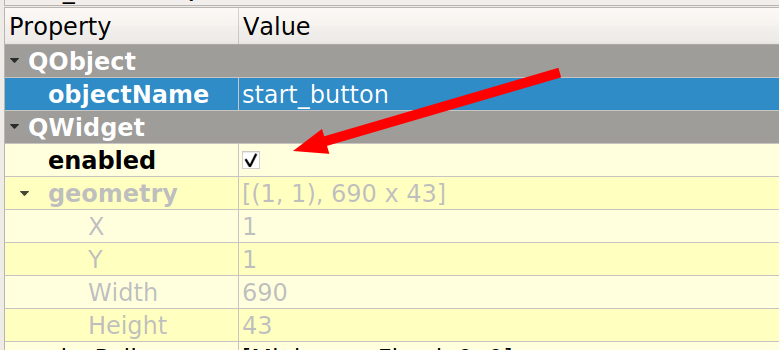
\includegraphics[width=.4\linewidth]{images/Chapter_09/10_enabled_button.png}
\end{center}

If you remove the tick mark from the option, the button gets grayed out, and you won't be able to click it. You must learn how to change the enabled status of our program, not from the Designer. For this, you must read the documentation provided by Qt. If you search online for \py{QPushButton}, usually, the first result would be the one available at \py{doc.qt.io}, the official documentation. You only need to be sure you're looking at the Qt5 documentation and not at the Qt4. The page is long, and if you look for \py{enabled}, you won't find anything. It's not a very auspicious start.

If you scroll to the top of the page, you see that Qt informs us of the parent class of QPushButton: QAbstractButton. Remember that when working with objects, there's always a possibility that methods and attributes are defined in the parent class, not in the class you're using. You can follow the link, but there won't be any information on enabling or not, but if you go one level above, to the \py{QWidget} documentation, you find what you were looking for:

\begin{center}
    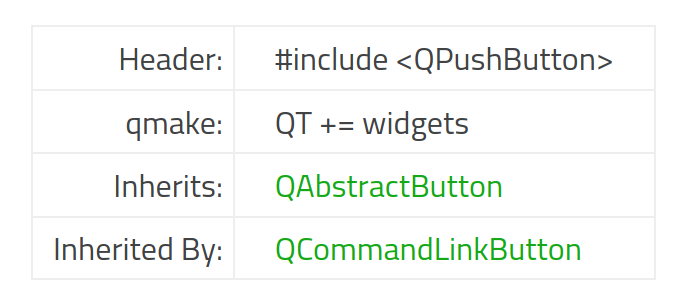
\includegraphics[width=.4\linewidth]{images/Chapter_09/11_Qt_Docs_inheritance.png}
\end{center}

To change the status of the button, you must use the \py{setEnabled()} method that is defined in the base \py{QWidget} class. On the one hand, you can notice that all widgets can be enabled or disabled. In some cases, the change is visible; in others, it won't be. You can also see that the Designer was already letting us know that the documentation was available as part of QWidget instead of QPushButton, just look at how it organizes the properties:

\begin{center}
    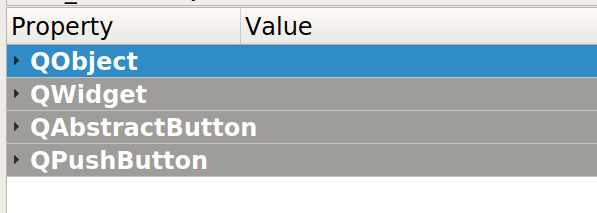
\includegraphics[width=.4\linewidth]{images/Chapter_09/12_Designer_object_inheritance.png}
\end{center}

Next time you want to learn how to do something, you know the best is to start by the Designer and see if the options are available. If you find it, you must pay attention to the base class that defines the behavior, and then you can go looking for the documentation. Navigating the Qt Docs takes a bit of getting used to, but once you understand how the information is organized, it becomes straightforward to follow it.

Back to the task at hand, you must disable the button when the scan starts running. One option would be to disable it right when you trigger the scan:

%! Suppress = Ellipsis
\begin{minted}{python}
    def start_scan(self):
        self.start_button.setEnabled(False)
        [...]
\end{minted}

It seems like a very valid idea until you use it for the first time. Once the scan starts, the button is grayed out, but there's no place where the button can be enabled back. It's a typical pattern with user interfaces. There are different ways to tackle the problem, but the more straightforward one is using the timer you already have in place to update the plot.

Instead of just plotting data, you can use the same timer to update the different elements of the user interface. For example, you would like to let the user start the scan only if there's no scan running, and you want to let them stop the scan only if there's one scan running. Let's start by defining a new method in the main window:

\begin{minted}{python}
    def update_gui(self):
        if self.experiment.is_running:
            self.start_button.setEnabled(False)
            self.stop_button.setEnabled(True)
        else:
            self.start_button.setEnabled(True)
            self.stop_button.setEnabled(False)
\end{minted}

The method \py{update_gui} is easy to follow. If the scan is running, you gray out one button but not the other and vice-versa. You only need to be sure this method runs periodically. Since you already have a timer for updating the plot, you can use it to update the GUI as well:

\begin{minted}{python}
    def __init__(self, experiment=None):
        self.timer.timeout.connect(self.update_gui)
\end{minted}

With this simple approach, you check every few milliseconds whether the scan is running or not, and you set the buttons accordingly. There's also a risk with this approach. If you decide to show information on the Main Window that implies reading a value from the device, you end up polling it several times per second, regardless of whether the value changed or not. If you update values stored in an object, such as the Experiment model, there's nothing to lose, but if you stretch this pattern too far, you may encounter issues, and our program could become inefficient.

You've generated the most basic of the possibilities, disabling a button to prevent the user from triggering a second scan if there's one already running. There are many more possibilities. What happens if the user enters a value outside the range. For example, as a start without volts, or negative, or beyond $3.3\,\textrm{V}$. You can use the \py{update_gui} to monitor the values entered and run them through some checks. If they pass, then you leave them as they are. If they don't, then you change the line to red and disable the start button.

All these are possibilities that you start considering as soon as you start developing user interfaces. However, everything you do has ramifications, such as what you saw when you disabled the start button on our first attempt. Our general approach is not to complicate the user interface beyond what is needed. If you've proper drivers and proper models in place, at least our devices are safe. If you find ourselves or a user of our software, making the same mistakes over and over again, you can then optimize the flow to prevent it from happening again.

\subsection{Saving data with a shortcut}\label{subsec:saving-data-with-a-shortcut}
The only missing important feature of our user interface is the ability to save data. You could implement a button for this, but you can also look into another important feature of Qt: \textbf{actions}. You saw that a convenient tool when developing with Qt are signals, such as the ones emitted by a button or a timer. Signals are associated with widgets of some sort. Another range is not associated with widgets, but the user can trigger them at any moment.

In the Designer, you can add a \py{File} menu, by double-clicking the top bar of the main window, where it says \py{Type Here}, and inside the File menu, you can create a \py{Save} option. As soon as you create the Save, the Designer also shows an \emph{Action} defined. You can find the action listed at the bottom of the right sidebar, as you show on the image below. Note that the name assigned by default is \py{actionSave}.

\begin{minipage}{0.45\linewidth}
    \centering
    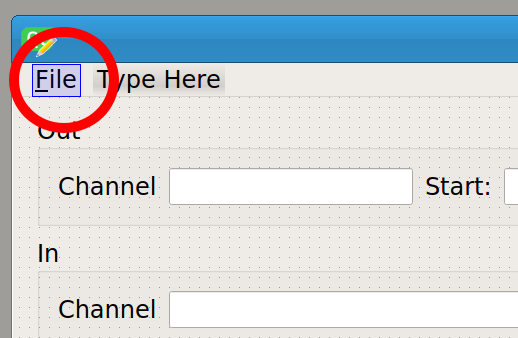
\includegraphics[width=\textwidth]{images/Chapter_09/13_menu_file.png}
\end{minipage}
\hspace{0.5cm}
\begin{minipage}{0.45\linewidth}
    \centering
    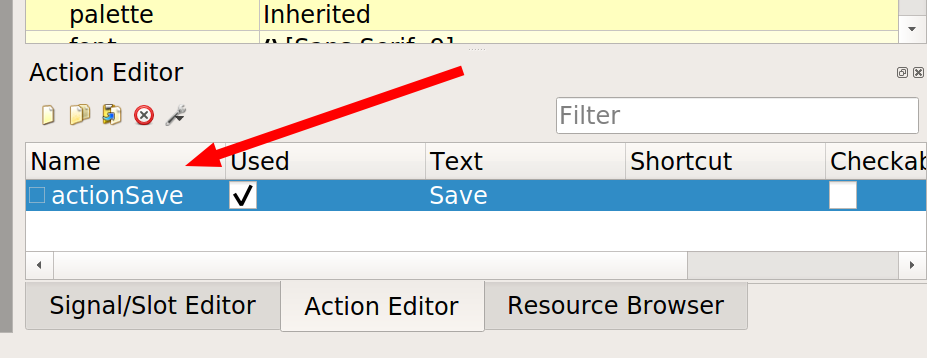
\includegraphics[width=\textwidth]{images/Chapter_09/13_action_save.png}
\end{minipage}

If you pay attention to what appears on that square, you see that there's also the possibility of defining a shortcut. You can go ahead, double-clicking on it opens a small configuration window in which you can add a shortcut, such as Ctrl+S. Just clicking on the shortcut edit line and then pressing a combination of keys register them. After saving, you can rerun the program, and you've a File menu with a Save option, and the shortcut written next to it, so there are no possible confusions.

You need to connect the \py{actionSave} to the method in our experiment for saving data. Because of how you structured the code, this now becomes almost trivial, in the \py{__init__} of the \py{MainWindow} you just add the following:

\mint{python}{self.actionSave.triggered.connect(self.experiment.save_data)}

You can use signals to trigger methods in other objects, not only in the window itself. When the experiment gets more complicated, it can be constructive just to trigger the model to do something than first defining a method on the window to trigger the model then. If you rerun the program, you can save the data either by going to File/Save or by pressing Ctrl+S. Go ahead and check the folder you specified in the config file, and you see the data appearing there.

\tipsInfo{Shortcuts}{Adding shortcuts for actions can be a good idea, but it also has risks. Shortcuts are hard to document, and some shortcuts are so universal that it's better not to re-define them. You could have used Ctrl+S to Start the scan. But then, you need to stop it and choose Ctrl+X, because it's right below. To save, you need to choose another shortcut and choose Ctrl+Q because it's on top of the S. All these shortcuts are generally used for something else, like saving, cutting, and closing a window. You're free to use them as you wish, but over usage leads to a perilous path.}

Of course, you may be tempted to open a pop-up dialog to ask for the folder where to save data. But again, this has a complex set of possibilities. If you open a pop-up every time you want to save data, it becomes annoying, especially if you save data often. If you show it only the first time, then you won't be able to change, later on, wondering why you showed it in the first place. It means you need to establish two behaviors: \emph{save} and \emph{save as}. You won't show how to do it here, but you leave it as an exercise:

\questionInfo{Exercise}{Qt bundles a \py{QFileDialog} widget, which allows the user to select a folder on the computer or create a new one. It can be used like this:

    \mint{python}{folder = QFileDialog.getExistingDirectory(self, 'Choose Folder')}

    Create a new action in the Designer to select the folder, and a new method in the main window to handle the selection of a directory to save the data.}

\section{Conclusions}\label{sec:conclusions}
This chapter is of great joy. It's the conclusion of a great journey, from developing a driver to creating models to abstract the behavior you expect both of the device and of the measurement you want to do, and finally to develop a user interface that works and looks beautiful.

This chapter focused on learning how to use the Qt Designer, a great tool to speed up the development of user interfaces. You covered the essential tools and patterns that one can expect to find in most user interfaces for scientific experiments. Qt, however, is a massive library that allows building almost anything, from the interface you see in some Mercedes cars to coffee vending machines, to programs running right now on your computer or mobile phone.

You've merely scratched the surface of what Qt offers. For scientific applications, however, you don't need to go much deeper. You're generally okay with the simple styling of the objects and a simple menu structure. You can change font-sizes, colors, the roundness of edges. You can make floating menus that open by right-clicking on an image, and many more things. But you always have to draw a line between how much effort and time you're dedicating to making a program look better and how much time you're dedicating to running an experiment.

\section{Where to Next}\label{sec:where-to-next}
If you reached this point, it means that you've kickstarted your career as a Scientific Python Developer, hurrah!. What you've covered in this book is only the beginning. Devices can be much more sophisticated than a simple DAQ, you may need to analyze the data before you display it, or the memory on our computer may not be enough to hold one complete measurement.

Our advice during the workshops is that you should work on what you've learned for at least 6 months—trying to develop solutions for the tools you already have at hand, such as an Oscilloscope, or your own data acquisition card. In this book, you've guided you; you've prevented you from falling in some errors. The reality is that you won't master any technique until you try by yourself, fail by yourself, and solve a problem by yourself.

To accompany you in this process, you've built a forum\footnote{available at: https://forum.pythonforthelab.com}.  You can ask any question related to programming, work in the lab, or Python. If you've any comments, suggestions, compliments, critiques to send us, you can do it directly to me at aquiles@pythonforthelab.com. I always want to read how your path is going, what topics are making you struggle.

If you're interested in a follow-up to this book, covering more advanced topics, please drop me a line. I am always seeking new ideas, topics, challenges, not only to produce content but to learn myself. I do a periodic braindump of what I learn on the website pythonforthelab.com. If anything grabs your attention, you can always leave a comment to let us know.

    \begin{appendices}
        \appendixpage
        \chapter{Python For The Lab {DAQ} Device Manual}\label{python-for-the-lab-daq-devicemanual}
We believe that learning how to program software for a scientific
laboratory can be achieved only through real-world examples. That is why
the course was conceived around a small device that we are calling a
General {DAQ} Device. In these pages, we document the behavior of the
device, in a similar way to what you would normally find in the manual
of any instrument in your own lab.

\section{Capabilities}\label{capabilities}
The \textbf{General {DAQ} Device} is a multi-purpose acquisition card
that can handle digital and analog inputs and outputs. It runs on an
{ARM} 32-bit microprocessor and drives its power from a {USB}
connection. The device can handle one task per turn, but the outputs are
persistent. This means that if you set the output of a particular port,
it will remain constant until a command for changing it is issued.

Normal Analog-to-Digital conversion times are in the order of 10
microseconds and are done with a resolution of 10 bits in the range
0-3.3V. Digital to Analog conversions are done with a resolution of 12
bits in the range 0-3.3V.

The {DAQ} possesses 2 Analog Output channels and 10 Analog Input
channels. Each can be addressed independently, however, a degree of
crosstalk can be observed, especially between neighboring ports.
Sensitive applications would, therefore, need to use non-consecutive
ports in order to mitigate this effect.

\section{Communication with a computer}\label{communication-with-acomputer}
The {DAQ} is able to communicate with the computer through a {USB}
connection. However the device has an onboard chip that converts the
communication into serial, therefore it will appear listed as any other
serial device.

The baud rate has to be set to 115200, and every command has to finish
with the newline {ASCII} character. The messages generated by the device
are also terminated by a newline character.

\section{List of Commands Available}\label{list-of-commandsavailable}
\textbf{{IDN}}: Identifies the device; returns a string with information
regarding the serial number and version of the firmware. \emph{Returns}:
String with information

\textbf{{OUT}:}: Command for setting the output of an analog channel. It
takes as arguments the channel \textbf{{CH}:\{\}} and the value,
\textbf{\{\textless{}4\}}. The value has to be in the range 0-4095,
while the channel has to be either 0 or 1.

\emph{Example}: {OUT}:{CH0}:1024

\textbf{{IN}}: Command for reading an analog input channel. It takes one
argument, \textbf{{CH}:\{\}}, between 0 and 9. \emph{Returns}: integer
in the range 0-1024

\emph{Example}: {IN}:{CH5}

\textbf{{DI}}: Command for identifying the device. It blinks a built-in LED 10 times.
It has no return.

\emph{Example}: {DI}

        \chapter{Review of Basic Operations with Python}\label{review-of-basic-operations-withpython}

\section{Chapter Objectives}\label{chapterobjectives}

The objective of \textbf{Python in the Lab} is to bring a developer from
knowing the basics of programming to being able to develop software for
controlling a complex setup. However, not all programmers have the same
background and it is important to establish a common ground from which
to start.

This chapter will quickly review how to start Python and how to interact
with it directly from the command line. It will also review some common
data structures such as lists and dictionaries. It will quickly go
through for loops and conditionals. If you are already familiar with
these concepts, you can safely skip this chapter.

\section{The Interpreter}\label{theinterpreter}
Python can be started from the command line by typing python and
pressing Enter. This should start the Python interpreter and you should
see something like this:

\begin{minted}{pycon}
Python 3.6.3 (default, Oct  3 2017, 21:45:48)
[GCC 7.2.0] on linux
Type "help", "copyright", "credits" or "license" for more information.
>>>
\end{minted}

You can type whatever you like into the interpreter. If it makes sense
to Python, it will give you an appropriate answer. For example, you
can do:

\begin{minted}{pycon}
>>> 2+3
5
\end{minted}

The first line is what you type (therefore it has the
\mintinline{pycon}{<<<} at the beginning),
while the second line is the output Python gives you (in this case, as
expected, \mintinline{pycon}{5}). You can go ahead and play with different
operations. You can multiply, subtract, divide, etc. Power of numbers
can be achieved using \mintinline{pycon}{**}, for example \mintinline{pycon}{2**.5} means the
square root of 2.

\section{Lists}\label{lists}
From now on, the \mintinline{pycon}{<<<}
will be suppressed in order to make it easier for you to copy the code.
Python can also be used to achieve much more complicated tasks and with
many different types of variables. For example, you can have a list and
iterate over every element of it:

\begin{minted}{python}
a = [1, 2, 3, 4]
for i in range(4):
    print(a[i])
\end{minted}

As you can see, \mintinline{pycon}{a} is a list with 4 elements. You make a
\mintinline{pycon}{for} loop over the four elements and you print them to screen.
You should see an output like this:

\begin{minted}{pycon}
1
2
3
4
\end{minted}

Of course, you can argue that this is not handy if you don't know
beforehand how many elements your list has. We can improve the code by
doing it like this:

\begin{minted}{python}
for i in range(len(a)):
    print(a[i])
\end{minted}

There is an important point to note, especially for those who come from
a Matlab kind of background. If you print the variable i inside the
loop, you'll notice it starts in 0 and goes all the way to N-1. It means
that the first element in a list is accessed by the index 0. Lists have
another interesting behavior. The elements in them do not need to be of
the same type. It is completely valid to do this:

\begin{minted}{python}
a = [1, 'a', 1.1]
for i in range(len(a)):
    print(type(a[i]))
### Output ###
<class 'int'>
<class 'str'>
<class 'float'>
\end{minted}

You can have lists with lists in them and many other combinations.

\exercise{Make a list in which each element is a list. Nesting two \mintinline{pycon}{for}
loops, display all the elements of all the lists.}

Lists can also be iterated over with a much simpler syntax, without the
need of the index.

\begin{minted}{python}
a = [1, 'a', 1.1]
for element in a:
    print(element)
\end{minted}

There is also a very \emph{pythonic} way of declaring lists with a very
concise syntax:

\begin{minted}{python}
a = [i for i in range(100)]
\end{minted}

This will generate a list of all the numbers from 0 to 99. You can also
calculate all the squares of those numbers with a small modification:

\begin{minted}{python}
a = [i**2 for i in range(100)]
\end{minted}

And you can make it even more complex, for example, if you want to get
only the even numbers you can type:

\begin{minted}{python}
a = [i for i in range(100) if i%2==0]
\end{minted}

\exercise{Given a list like: \mintinline{pycon}{b = [1, 2, 'a', 3, 4, 'b', 5, 'c', 'd']}, create
another list with only the elements of type string.}

Lists are a fundamental Python structure and it is important to keep
them in mind in order to follow the syntax of some programs without
getting lost.

\section{Dictionaries}\label{dictionaries}
Dictionaries are one of the most useful data structures of Python. They
are somehow like lists, but instead of accessing them via a numerical
index they are accessed via a string identifier. For example, you can
generate a dictionary and access its values by doing:

\begin{minted}{python}
a = {'first': 1, 'second': 2}
a['first']
\end{minted}

Dictionaries, as lists, can store different types of variables in them.
Pay attention to the definition and call: lists are defined using square
brackets \mintinline{pycon}{[} \mintinline{pycon}{]}, while dictionaries are defined with
curly brackets \mintinline{pycon}{{}}. However, for accessing an
element the square brackets are used. It is possible therefore to do:

\begin{minted}{python}
b = [1, 2, 3, '4', 5.1]
a = {'first': 1, 'second': b}
a['second']
\end{minted}

The first notable advantage of using dictionaries is that it makes much
clearer what data you are storing. You are giving a title to a specific
value. If you want to calculate the area of a triangle:

\begin{minted}{python}
t = {'base': 2, 'height': 1}
area = t['base']*t['height']/2
\end{minted}

And you immediately see that even if you don't have the definition of
\mintinline{pycon}{t}, it is very clear what you are doing. It is clearer than the
following code:

\begin{minted}{python}
area = t[0]*t[1]/2
\end{minted}

In the case of a triangle, it doesn't really matter which element is the
base and which one is the height. However, for more complex
applications, altering the order can have very serious consequences. In
the same fashion than with lists, it is possible to access every element
within a for loop:

\begin{minted}{python}
for key in a:
    print(key)
    print(a[key])
\end{minted}

Now the key has a value that can be printed and used. We can also check
if a specific key is present in the dictionary:

\begin{minted}{python}
if 'first' in a:
    print('First is in a')
\end{minted}

If you want to update several values of a dictionary, but not to replace
the dictionary itself, you can use the command \mintinline{pycon}{update}:

\begin{minted}{python}
a = {'first': 1, 'second': 2, 'third': 3}
new_values = {'first': 5, 'second': 6, 'fourth': 4}
a.update(new_values)
a['first']
a['third']
a['fourth']
\end{minted}

If you pay attention you will see that not only the already existent
values were updated, but a new one was created.

\exercise{Given two dictionaries, 
\mint{python}|a = {'first': 1, 'second': 2, 'third': 3}| 
and
\mint{python}|b = {'fourth': 4, 'fifth': 5}|
merge the second into the first one.}

Of course, it is also possible to delete an element from a dictionary:

\begin{minted}{python}
a = {'first': 1, 'second': 2, 'third': 3}
del a['first']
print(a['first'])
\end{minted}

You'll see an error letting you know that the key \mintinline{pycon}{first} is not
in the dictionary. So far we have always used \mintinline{pycon}{strings} for the
keys of the dictionary, but nothing prevents you from using numbers. The
following lines are perfectly valid:

\begin{minted}{python}
a = {1: 2, 2:4, 3: 9}
b = {0.1: 2, 'a': 3, 1:1}
\end{minted}

This, on one hand, makes dictionaries very versatile, on the other, it
may make the code slightly more confusing. For example \mintinline{pycon}{a[1]}
may be referring to either the second element of a list or the element
of a dictionary with key \mintinline{pycon}{1}. At this point, you may wonder why
you would use lists if dictionaries give you even more functionality.
The short answer is memory usage; the code below will output the memory
being used by a dictionary and by a list with the same information in
them. The first line of the code is just importing the function we need
for calculating the size of a variable.

\begin{minted}{python}
from sys import getsizeof

a = [i for i in range(100)]
b = {i:i for i in range(100)}

print(getsizeof(a))
print(getsizeof(b))
\end{minted}

You should see that the size of \mintinline{pycon}{a} is \mintinline{pycon}{912\ bytes} while
the size of the dictionary \mintinline{pycon}{b} is \mintinline{pycon}{4704\ bytes}. Even if
you consider that the dictionary is storing not only the value but also
the key, the ratio of memory usage of a dictionary to a list is more
than twice.

\exercise{Write a simple for loop that prints the ratio of the memory usage of a
list and of a dictionary as a function of the length of each.}

        \chapter{Classes in Python}\label{classes-in-python}
Python is an object oriented programming (OOP) language. Object oriented
programming is a programming design that allows developers not only to
define the type of data of a variable but also the operations that can
act on that data. For example, a variable can be of type integer, float,
string, etc. We know that we can multiply an integer to another, or
divide a float by another, but that we cannot add an integer to a
string. Objects allow programmers to define operations both between
different objects as with themselves. For example, we can define an object
\mintinline{python}{person}, add a birthday and have a function that returns the
person's age.

At the beginning it will not be clear why objects are useful, but over
time it becomes impossible not to think with objects in mind. Python
takes the objects ideas one step further, and considers every variable
an object. Even if you didn't realize, it is possible that you have
already encountered some of these ideas when working with numpy arrays,
for example. In this chapter we are going to cover from the very basics
of object design to slightly more advanced topics in which we can define a 
custom behavior for most of the common operations.

\section{Defining a Class}\label{defining-a-class}
Let's dive straight into how to work with classes in Python. Defining a class is as
simple as doing:

\begin{minted}{python}
class Person():
    pass
\end{minted}

When speaking it is very hard not to interchange the words
\mintinline{python}{Class} and \mintinline{python}{Object}. The reality is that the difference
between them is very subtle: an object is an instance of a class. This
means that we will use classes when referring to the type of variable,
while object to the variable itself. It is going to be come clearer
later on.

In the example above, we've defined a class called \mintinline{python}{Person} that doesn't do
anything (that is way it says \mintinline{python}{pass}.) We can add more
functionality to this class by declaring a function that belongs to it. Create a file called \textbf{person.py} and add the following code to it:

\begin{minted}{python}
class Person():
    def echo_name(self, name):
        return name
\end{minted}

In Python, the functions that belong to classes are called \textbf{methods}. For
using the class, we have to create a variable of type person. Back in the Python Interactive Console, you can, for example, do:

\begin{minted}{pycon}
>>> from person import Person
>>> me = Person()
>>> me.echo_name("John Snow")
\end{minted}

The first line imports the code into the interactive console. For this to work, it is important that you trigger python directly from the same folder where the file \textbf{person.py} is located. When you run the code above, you should see as output \mintinline{python}{John Snow}. There is also an
important detail that was ommitted this far, the presence of
\mintinline{python}{self} in the delcaration of the method. All the methods in
python take a first input variable called self, referring to the class
itself. For the time being don't stress yourself about it, but bear in
mind that when you define a new method, you should always include the
\mintinline{python}{self}, but when calling the method you should never include it.
You can also write methods that don't take any input, but still will
have the \mintinline{python}{self} in them, for example:

\begin{minted}{python}
def echo_True(self):
    return "True"
\end{minted}

that can be used by doing:

\begin{minted}{pycon}
>>> me.echo_True()
\end{minted}

So far, definig a function within a class has no advantage at all. The
main difference, and the point where methods become handy is because
they have access to all the information stored within the object itself.
The \mintinline{python}{self} argument that we are passing as first argument of the
function is exactly that. For example, we can add the following two
methods to our class Person:

\begin{minted}{python}
def store_name(self, name):
    self.stored_name = name

def get_name(self):
    return self.stored_name
\end{minted}

And then we can execute this:

\begin{minted}{pycon}
>>> me = Person()
>>> me.store_name('John Snow')
>>> print(me.get_name())
>>> print(me.stored_name)
\end{minted}

What you can see in this example is that the method \mintinline{python}{store_name}
takes one argument, \mintinline{python}{name} and stores it into the class variable
\mintinline{python}{stored_name}. As with methods, variables are called \textbf{properties}
in the context of a class. The method \mintinline{python}{get_name} just returns
the stored property. What we show in the last line is that we can access
the property directly, without the need to call the \mintinline{python}{get_name}
method. In the same way, we don't need to use the \mintinline{python}{store_name}
method if we do:

\begin{minted}{pycon}
>>> me.stored_name = 'Jane Doe'
>>> print(me.get_name())
\end{minted}

One of the advantages of the attributes of classes is that they can be
of any type, even other classes. Imagine that you have acquired a timetrace
of an analog sensor and you have also recorded the temperature of the
room when the measurement started. You can easily store that information
in an object:

\begin{minted}{python}
measurement.temperature = '20 degrees'
measurement.timetrace = np.array([...])
\end{minted}

What you have so far is a vague idea of how classes behave, and maybe
you are starting to imagine some places where you can use a class to
make your daily life easier and your code more reusable. However, this
is just the tip of the iceberg. Classes are very powerfull
tools.

\section{Initializing classes}\label{initializing-classes}
Instantiating a class is the moment in which we call the class and pass
it to a variable. In the previous example, the instantiation of the
class happened at the line reading \mintinline{python}{me = Person()}. You may
have noticed that the property \mintinline{python}{stored_name} does not exist in
the object until we assign a value to it. This can give very serious
headaches if someone calls the method \mintinline{python}{get_name} before actually
having a name stored (you can give it a try to see what happens!)
Therefore it is very useful to run a default method when the class is
first called. This method is called \mintinline{python}{__init__}, and you can
use it like this:

\begin{minted}{python}
class Person():
    def __init__(self):
        self.stored_name = ""

    [...]
\end{minted}

If you go ahead and run the \mintinline{python}{get_name} without actually storing
a name beforehand, now there will be no error, just an empty string
being returned. While initializing you can also force the execution of
other methods, for example:

\begin{minted}{python}
def __init__(self):
    self.store_name('')
\end{minted}

Will have the same final effect. It is however common (and smart)
practice, to declare all the variables of your class at the beginning,
inside your \mintinline{python}{__init__}. In this way you don't depend on
specific methods being called to create the variables. 

As with any other method, you can have an \mintinline{python}{__init__} method with more
arguments than just \mintinline{python}{self}. For example you can define it like
this:

\begin{minted}{python}
def __init__(self, name):
    self.stored_name = name
\end{minted}

Now the way you instantiate the class is different, you will have to do
it like this:

\begin{minted}{python}
me = Person('John Snow')
print(me.get_name())
\end{minted}

When you do this, your previous code will stop working, because now you have to set the \mintinline{python}{name} explicitly. If there is any other code that does \mintinline{python}{Person()} will fail. The proper way of altering the functioning of a method is to add a default value in case no explicit value is passed. The \mintinline{python}{__init__} would become:

\begin{minted}{python}
def __init__(self, name=''):
    self.stored_name = name
\end{minted}

With this modification, if you don't explicitly specify a name when instantiating the class, it will default to \py{''}, i.e., an empty string.

\exercise{Improve the \mintinline{python}{get_name} method in order to print a warning message in case the name was not set}

\section{Defining class properties}
So far, if you wanted to have properties available right after the instantiation of a class, you had to include them in the \py{__init__} method. However, this is not the only possibility. You can define properties that belong to the class itself. Doing it is as simple as declaring them before the \py{__init__} method. For example, we could do this:

\begin{minted}{python}
class Person():
    birthday = '2010-10-10'
    def __init__(self, name=''):
        [...]
\end{minted}

If you use the new \py{Person} class, you will have a property called \py{birthday} available, but with some interesting behavior. Let's see. First, let's start as always:

\begin{minted}{pycon}
>>> from person import Person
>>> guy = Person('John Snow')
>>> print(guy.birthday)
2010-10-10
\end{minted}

What you see above is that it doesn't matter if you define the birthday within the \py{__init__} method or before, when you instantiate the class, you access the property in the same way. The main difference is what happens before instantiating the class:

\begin{minted}{pycon}
>>> from person import Person
>>> print(Person.birthday)
2010-10-10
>>> Person.birthday = '2011-11-11'
>>> new_guy = Person('Cersei Lannister')
>>> print(new_guy.birthday)
2011-11-11
\end{minted}

What you can see in the code above is that you can access class properties before you instantiate anything. That is why they are class and not object properties. Subtetlies apart, once you change the class property, in the example above the birtday, next time we create an object with that class it will receive the new property. At the beginning it is hard to understand why it is useful, but one day you will need it and it will save you a lot of time. 

\section{Inheritance}
One of the advantages of working with classes in Pythan is that it allows you to use the code from other developers and expand or change its behavior without modifying the original code. The best would be to see it in action. So far we have a class called \py{Person}, which is general but not too useful. Let's assume we want to define a new class, called \py{Teacher}, that has the same properties as a \py{Person} (i.e., name and birthday) plus it is able to teach a class. You can add the following code to the file \textbf{person.py}:

\begin{minted}{python}
class Teacher(Person):
    def __init__(self, course):
        self.course = course
        
    def get_course(self):
        return self.course
        
    def set_course(self, new_course):
        self.course = new_course
\end{minted}

Note that in the definition of the new \py{Teacher} class, we have added already \py{Person}. In Python jargon, this means that the class \py{Teacher} is a child of the class \py{Person}, or viceversa, that \py{Person} is the parent of \py{Teacher}. This is called \textbf{inheritance} and is not only very common in Python programs, it is one of the characteristics that makes Python so versatile. You can use the class \py{Teacher} in the same way as you have used the class \py{Person}:

\begin{minted}{pycon}
>>> from person import Teacher
>>> me = Teacher('math')
>>> print(me.get_course)
math
>>> print(me.birthday)
2010-10-10
\end{minted}

However, if you try to use the teacher's name it is going to fail:

\begin{minted}{pycon}
>>> print(me.get_name())
[...]
AttributeError: 'Teacher' object has no attribute 'stored_name'
\end{minted}

The reason behind this error is that \py{get_name} returns \py{stored_name} in the class Person. However, the property \py{stored_name} is created when running the \py{__init__} method of Person, which didn't happen. You could have changed the code above slightly to make it work: 

\begin{minted}{pycon}
>>> from person import Teacher
>>> me = Teacher('math')
>>> me.store_name('J.J.R.T.')
>>> print(me.get_course)
math
>>> print(me.get_name())
J.J.R.T.
\end{minted}

However, there is also another approach to avoid the error. You could simply run the \py{__init__} method of the parent class (i.e. the base class), you need to add the follwing:

\begin{minted}{python}
class Teacher(Person):
    def __init__(self, course):
        super().__init__()
        self.course = course
    [...]
\end{minted}

When you use \py{super()}, you are going to have access directly to the class from which you are inheriting. In the example above, you explicitly called the \py{__init__} method of the parent class. If you try again to run the method \py{me.get_name()}, you will see that no error appears, but also that nothing is printed to screen. This is because you triggered the \py{super().__init__()} without any arguments and therefore the name defaulted to the empty string. 

\exercise{Improve the \py{Teacher} class in order to be able to specify a name to it when instantiating, for example, you would like to do this: \mintinline{pycon}{Teacher('Red Sparrow', 'Math')}}

\section{Finer details of classes}
With what you have learned up to here, you can achieve a lot of things, it is just a matter of thinking how to connect different methods, when it is useful to inherit. Wihtout doubts, it will help you to understand the code developed by others. There are, however, some details that are worth mentioning, because you can improve how your classes look and behave. 

\subsection{Printing objects}
Let's see, for example, what happens if you print an object:
\begin{minted}{pycon}
>>> from person import Person
>>> guy = Person('John Snow')
>>> print(guy)
<__main__.Student object at 0x7f0fcd52c7b8>
\end{minted}
The output of printing \py{guy} is quite ugly and is not particularly useful. Fortunately, you can control what appears on the screen. You have to update the \py{Person} class. Add the following method to the end:

\begin{minted}{python}
def __str__(self):
    return "Person class with name {}".format(self.stored_name)
\end{minted}

If you run the code above, you will get the following:
\begin{minted}{pycon}
>>> print(guy)
Person class with name John Snow
\end{minted}

You can get very creative. It is also important to point out that the method \py{__str__} will be used also when you want to transform an object into a string, for example like this:

\begin{minted}{pycon}
>>> class_str = str(guy)
>>> print(class_str)
Person class with name John Snow
\end{minted}

Which also works if you do this:

\begin{minted}{pycon}
>>> print('My class is {}.'.format(guy))
\end{minted}

Something that is important to point out is that this method is inherited. Therefore, if you, instead of printing a \py{Person}, print a \py{Student}, you will see the same output, which may or may not be the desired behavior.

\subsection{Defining complex properties}
When you are developing complex classes, sometimes you would like to alter the behavior of assigning values to an attribute. For example you would like to change the age of a person when you store the year of birth:
\begin{minted}{pycon}
>>> person.year_of_birth = 1980
>>> print(person.age)
38
\end{minted}

There is a way of doing this in Python which can be easily implemented even if you don't fully understand the syntax. Working again in the class \py{Person}, we can do the following:
\begin{minted}{python}
class Person():
    def __init__(self, name=None):
        self.stored_name = name
        self._year_of_birth = 0
        self.age = 0

    @property
    def year_of_birth(self):
        return self._year_of_birth
        
    @year_of_birth.setter
    def year_of_birth(self, year)
        self.age = 2018 - year
        self._year_of_birth = year
\end{minted}
Which can be used like this:
\begin{minted}{pycon}
>>> from people import Person
>>> me = Person('Me')
>>> me.age
0
>>> me.year_of_birth = 1980
>>> me.age
32
\end{minted}

What is happening is that Python gives you control over everything, including what does the \py{=} do when you assign a value to an attribute of a class. The first time you create a \py{@property}, you need to specify a function that returns a value. In the case above, we are returning \py{self._year_of_birth}. Just doing that will allow you to use \py{me.year_of_birth} as any attribute, but it will fail if you try to change its value. This is called a read-only property. If you are working in the lab, it is useful to define methods as read-only properties when you can't change the value. For example, a method for reading the serial number would be read-only. 

If you want to change the value of a property, you have to define a new method. This method is going to be called a \textit{setter}. That is why you can see the line \py{@year_of_birth.setter}. The method takes an argument that triggers two actions. On the one hand, it updates the age, on the other it stores the year in an attribute. It takes a while to get used to, but it can be very handy. It takes a bit more of time to develop than with simple methods, but it simplifies a lot the rest of the programs that build upon the class. 

    \end{appendices}

\end{document}
